\documentclass[%draft,
    10pt,
    headinclude, footexclude,
    % twoside, % this produces strange margins!
    openright, % for new chapters
    notitlepage,
    cleardoubleempty,
    headsepline,
    pointlessnumbers,
    bibtotoc, idxtotoc,
    ]{scrbook}

% iPad Air 2 resolution: 1536 x 2048
% 1.3333 ratio (4:3)
% LeeSeshia is 15,73 ? 20,96 cm, ratio 1.332
%\setlength{\paperwidth}{15.73cm} \setlength{\paperheight}{20.96cm}
\setlength{\paperwidth}{15.72cm} \setlength{\paperheight}{20.95cm}
%\typearea{calc} % without BCOR results to a DIV of 8 for 11pt
\typearea[1.1cm]{15} % used 18, but 15 gives more space for the binding, TODO: check if 1.1 cm is the correct number

\usepackage{scrlayer-scrpage}
\setkomafont{pagehead}{\scshape\small}
\setkomafont{pagenumber}{\scshape\small}


\newif\ifbook
%\booktrue % comment out for the print book version

\ifbook
\else
\ifoot{\hyperlink{contents}{{\textnormal{Contents}}}}
\cfoot{\hyperlink{index}{{\textnormal{Index}}}}
\fi



\usepackage{pslatex} % -- times instead of computer modern, especially for the plain article class
\usepackage[pdftex,
            pdfauthor={Martin Schoeberl},
            pdftitle={Digital Design with Chisel},
            colorlinks=true,bookmarks=true]{hyperref}

\usepackage{booktabs}
\usepackage{graphicx}
\usepackage{xcolor}
\usepackage{multirow}
\usepackage{cite}
\usepackage{dirtree}
\usepackage{pdfpages}
\usepackage{makeidx}
%\usepackage{showidx} % for index debugging
% For alignment on tables
\usepackage{dcolumn}
\newcommand{\cc}[1]{\multicolumn{1}{c}{#1}}
\usepackage{tikz}
\usetikzlibrary{arrows,bending}
\usetikzlibrary{positioning}


% fatter TT font
\renewcommand*\ttdefault{txtt}
% another TT, suggested by Alex
% \usepackage{inconsolata}
% \usepackage[T1]{fontenc} % needed as well?

% Smaller verbatim text
\usepackage{etoolbox}
\makeatletter
\patchcmd{\@verbatim}
  {\verbatim@font}
  {\verbatim@font\small}
  {}{}
\makeatother

\usepackage[procnames]{listings}


\ifbook
\hypersetup{
  linkcolor  = black,
  citecolor  = black,
  urlcolor   = black,
  colorlinks = black,
  bookmarks=false,
}
\else
\hypersetup{
  linkcolor  = blue,
  citecolor  = blue,
  urlcolor   = blue,
  colorlinks = true,
  bookmarks=true,
  pdfpagemode=UseOutlines,
}
\fi


\makeindex

% not really used
\newenvironment{comment}
{ \vspace{-0.1in}
  \begin{quotation}
  \noindent
  \small \em
  \rule{\linewidth}{0.5pt}\\
}
{
  \\
  \rule{\linewidth}{0.5pt}
  \end{quotation}
}

\newcommand{\scale}{0.7}

\input{shared/chisel.tex}

\newcommand{\code}[1]{{\lstinline[basicstyle=\small\ttfamily]{#1}}}
\newcommand{\codefoot}[1]{{\lstinline[basicstyle=\footnotesize\ttfamily]{#1}}}

\newcommand{\todo}[1]{{\emph{TODO: #1}}}
\newcommand{\martin}[1]{{\color{blue} Martin: #1}}
\newcommand{\myref}[2]{\href{#1}{#2}}

\ifbook
\renewcommand{\myref}[2]{{#2}{\footnote{\url{#1}}}}
\fi

% uncomment following for final submission
%\renewcommand{\todo}[1]{}
%\renewcommand{\martin}[1]{}

\makeindex

\begin{document}


\ifbook
\else
\includepdf{chisel-cover.pdf}
\newpage
\thispagestyle{empty}
~
\newpage
\fi



\begin{flushleft}
\pagestyle{empty}
\ \\
\vspace{1cm}
{\usekomafont{title}\mdseries\huge Digital Design with Chisel}
\ \\
\vspace{1cm}
{\usekomafont{title}\mdseries\Large Sixth Edition}
\cleardoublepage
\end{flushleft}
\newpage


\begin{flushleft}
\pagestyle{empty}
\ \\
\vspace{1cm}
{\usekomafont{title}\Huge Digital Design with Chisel\\
\bigskip
{\usekomafont{title}\huge Sixth Edition}\\
\bigskip
\bigskip
\bigskip
\bigskip
%{\large\itshape Beta Edition}\\
\bigskip
{\usekomafont{title}\huge Martin Schoeberl}
\medskip\\
%{\large\itshape martin@jopdesign.com}

}

%\vspace{10cm} \emph{Version: \today}
\newpage
\end{flushleft}

\thispagestyle{empty}
\begin{flushleft}
{\small

%\lowertitleback{
Copyright \copyright{} 2016--2024 Martin Schoeberl
  \medskip\\
  \begin{tabular}{lp{.8\textwidth}}
    \raisebox{-12pt}{\includegraphics[height=18pt]{figures/cc_by_sa}} &
     This work is licensed under a Creative Commons Attribution-ShareAlike
     4.0 International License.
     \url{http://creativecommons.org/licenses/by-sa/4.0/}\\
  \end{tabular}
%}

\medskip

Email: \url{martin@jopdesign.com}\\
Visit the source at \url{https://github.com/schoeberl/chisel-book}
\medskip

First edition published 2019 by Kindle Direct Publishing,\\
\url{https://kdp.amazon.com/}
\medskip
\medskip


\textbf{Library of Congress Cataloging-in-Publication Data}
\medskip

Schoeberl, Martin
\begin{quote}
Digital Design with Chisel\\
Martin Schoeberl\\
Includes bibliographical references and an index.\\
ISBN 9781689336031
\end{quote}

\bigskip


Manufactured in the United States of America.

Typeset by Martin Schoeberl.}
\end{flushleft}

\frontmatter

\phantomsection
\hypertarget{contents}{}
\tableofcontents


\begingroup
\let\cleardoublepage\clearpage
\listoffigures
\listoftables
\lstlistoflistings
\endgroup

\chapter{Foreword}

\medskip
\medskip

It is an exciting time to be in the world of digital design. With the end of Dennard Scaling and the slowing of Moore's Law, there has perhaps never been a greater need for innovation in the field. Semiconductor companies continue to squeeze out every drop of performance they can, but the cost of these improvements has been rising drastically. Chisel reduces this cost by improving productivity. If designers can build more in less time, while amortizing the cost of verification through reuse, companies can spend less on Non-Recurring Engineering (NRE). In addition, both students and individual contributors can innovate more easily on their own.

Chisel is unlike most languages in that it is embedded in another programming language, Scala. Fundamentally, Chisel is a library of classes and functions representing the primitives necessary to express synchronous, digital circuits. A Chisel design is really a Scala program that \emph{generates} a circuit as it executes. To many, this may seem counterintuitive: ``Why not just make Chisel a stand-alone language like VHDL or SystemVerilog?'' My answer to this question is as follows: the software world has seen a substantial amount of innovation in design methodology in the past couple of decades. Rather than attempting to adapt these techniques to a new hardware language, we can simply \emph{use} a modern programming language and gain those benefits for free.

A longstanding criticism of Chisel is that it is ``difficult to learn.'' Much of this perception is due to the prevalence of large, complex designs created by experts to solve their own research or commercial needs. When learning a popular language like C++, one does not start by reading the source code of GCC. Rather, there are a plethora of courses, textbooks, and other learning materials that cater toward newcomers. In \emph{Digital Design with Chisel}, Martin has created an important resource for anyone who wishes to learn Chisel.

Martin is an experienced educator, and it shows in the organization of this book. Starting with installation and primitives, he builds the reader's understanding like a building, brick-by-brick. The included exercises are the mortar that solidifies understanding, ensuring that each concept sets in the reader's mind. The book culminates with \emph{hardware generators} like a roof giving the rest of the structure purpose. At the end, the reader is left with the knowledge to build a simple, yet useful design: a RISC processor.

In \emph{Digital Design with Chisel}, Martin has laid a strong foundation for productive digital design. What you build with it is up to you.

\medskip
\noindent Jack Koenig\\
Chisel and FIRRTL Maintainer\\
Staff Engineer, SiFive


\chapter{Preface}

% This text goes on the backside of the book, and in Amazon description
This book is an introduction to digital design with a focus on using the hardware construction language Chisel. Chisel brings advances from software engineering, such as object-orientated and functional languages, into digital design.

This book addresses hardware designers and software engineers. Hardware designers with knowledge of Verilog or VHDL can upgrade their productivity with a modern language for their next ASIC or FPGA design. Software engineers with knowledge of object-oriented and functional programming can leverage their knowledge to program hardware, for example, FPGA accelerators executing in the cloud.

The approach of this book is to present small to medium-sized typical hardware components to explore digital design with Chisel.

% about me, backside

%Martin Schoeberl is Associate Professor at the Technical University of Denmark, where he is teaching digital electronics and computer architecture. His research interest is on hard real-time systems, time-predictable computer architecture, and real-time Java. He has more than 100 publications in peer reviewed journals, conferences, and books.

%Martin has been four times at UC Berkeley on research stays, where he has picked up Chisel and was in close contact with the developers of Chisel. He lead the research project T-CREST where most of the components have been written in Chisel.

\section*{Foreword for the Second Edition}

As Chisel allows agile hardware design, so does open access and on-demand printing
allow agile textbook publishing. Less than 6 months after the first edition of this book
I am able to provide an improved and extended second edition.

Besides minor fixes, the main changes in the second edition are as follows.
The testing section has been extended. The sequential building blocks chapter contains
more example circuits. A new chapter on input processing explains input synchronization,
shows how to design a debouncing circuit, and how to filter a noisy input signal.
The example designs chapter has been extended to show different implementations of a FIFO.
The FIFO variations also show how to use type parameters and inheritance in digital design.

\section*{Foreword for the Third Edition}

Chisel has been moving forward in the last year, so it is time for a new edition of the Chisel book.
We changed all examples to the latest version of Chisel (3.5.3), and the recommended
Scala version (2.12.13).

With Chisel 3.5 the testing environment \code{PeekPokeTester} as part of the \code{iotesters}
package has been deprecated. Therefore, we have changed the testing description to the new
\myref{https://github.com/ucb-bar/chiseltest}{ChiselTest} framework.
As there are still many Chisel designs available that use the \code{PeekPokeTester},
we have moved the description for it into the appendix.

One of the fascinating aspects of the Chisel/Scala/Java environment is that we
can piggyback on the available infrastructure to distribute open-source libraries.
We can publish hardware components on Maven as simply as any other open-source Java library.
Publishing on Maven means that a 3rd party component can be integrated into the
compile flow with a single reference in the \code{build.sbt} configuration.
This is the same process as how you include the chisel library for your design.
We have added a section on how to publish a Chisel design on Maven Central.

We have improved the explanation of components with a simpler example.

Hardware \emph{generators} are written in Scala. Therefore, we have added a short
section on Scala. We have extended the hardware generator chapter with a section
on using functional programming to write generators.

The appendix has been extended with a list of reserved keywords and a list
of acronyms.

Hans Jakob Damsgaard has contributed the description of how to use external components, through Chisel's \code{BlackBox}, and how to use memories for clock domain crossing
(multi-clock memories).

\section*{Foreword for the Fourth Edition}

For the fourth edition, we have switched to the actual Chisel version 3.5.4.
We have added arbiter, priority encoder, and comparator to the chapter of
combinational building blocks.
We have extended the hardware generation chapter with more functional
examples, including building a fair arbitration tree out of a simple 2 to 1
arbitration circuits.
We have added a new chapter on interconnect, bus interfaces,
and how to connect an IO device as a memory-mapped device.
We have started a new chapter on debugging, testing, and verification.
The plan is to extend the chapter on this important topic in the next edition.
We have extended the processor chapter with a more gentle introduction
to a microprocessor, including a figure of the datapath.

\section*{Foreword for the Fifth Edition}

For the fifth edition, we have upgraded to the actual Chisel version 3.5.6 and Scala 2.13.
To make room for more advanced topics, I have removed the two appendicitis on
Chisel 2 and the PeekPokeTester. All projects that are actively maintained have finally
moved to Chisel 3, at least with the compatibility layer. The PeekPokeTester has been
deprecated with Chisel 3.5 and it is recommended to switch to ChiselTest.
If needed, those two chapters are available in the older versions of the Chisel book,
available as PDF at the \myref{https://www.imm.dtu.dk/~masca/chisel-book.html}{web page} for this book.

The fifth edition does not include major changes; it is a consolidation version.
We did considerable proofreading for more clarity in writing. Chisel has added small convenience
features (e.g., \code{ChiselEnum}) that we cover in this edition.
We extended the processor chapter and updated the Leros code snippets
to the actual version of Leros.


\section*{Foreword for the Sixth Edition}


Chisel has recently gone through some major changes. Up to Chisel 3.x, Chisel is mainly
based on Scala, which means it runs on the Java virtual machine and is platform independent.
After 3.x Chisel the architecture of the Chisel compile pipeline has changed. To indicate that change,
the version numbering system has change to increment that major version number more often.
Version 4.0 is skipped and the next Chisel version is 5.0.
From 5.0 the compiler backend is based on \myref{https://circt.llvm.org/}{CIRCT},
a circuit compiler, which is part of the \myref{https://llvm.org/}{LLVM} project.
The main difference for the Chisel user is that CIRCT (and LLVM) are written in C++
and therefore need a different executable for each operating system (processor
architecture).


We tested the book with following Chisel Versions: 3.5.6, 3.6.1, 5.3.0, and 6.5.0.
Chisel 3.6 is the last that uses the Scala based backend to produce Verilog files.
Chisel 5 is using CIRCT and needs \code{firtool} installed.
The latest version of Chisel 6 includes the \code{firtool} binaries.
Testing with ChiselTest is still supported until Chisel 6.
Chisel 6 might switch to a different simulation and testing library.
We use Scala 2.13 and tested with Java 17.
Note that Java 21 is currently not supported by \code{sbt}.


\todo{Some of this might go into getting started.}




\todo{We should also show more Leros code.}

\todo{VHDL and Verilog}


We extended the testing chapter with a description how to access internal signals. \todo{That is too
little to be mentioned here. More is needed.}

Assertions and Chisel formal (if finished).






\section*{Translations}

This book has been translated to Chinese, Japanese, and Vietnamese. All translations are available as free PDF
from the books \myref{https://www.imm.dtu.dk/~masca/chisel-book.html}{web page}.
I would like to thank Yuda Wang, Qiwei Sun, and Yun Chen for the Chinese translation;
Seiji Munetoh, Masatoshi Tanabata, and Takaaki Hagino for the Japanese translation;
and VieLe Duc Hung for the Vietnamese translation.
If you are interested to translate this book into another language, feel free to do it and
publish it under the same license. Please contact me then, so I can point to your translation.


\section*{Acknowledgements}

I want to thank everyone who has worked on Chisel for creating such
a cool hardware construction language. Chisel is so joyful to use and
therefore worth writing a book about.
I am thankful to the whole Chisel community, which is so welcoming and friendly
and never tired to answer questions on Chisel.

I would also like to thank my students in the last years of an advanced computer
architecture course where most of them picked up Chisel for the final project.
Thank you for moving out of your comfort zone and taking up the journey of
learning and using a bleeding-edge hardware description language.
Many of your questions have helped to shape this book.

It was a pleasure to use Chisel in teaching a digital electronics
course at the Technical University of Denmark since 2020.
I know it is a challenge to pickup Chisel and Java in parallel in the second
semester. Thank you to all students from this course, who had on open mind to
pickup a modern programming language for hardware description.

For the third edition, I would like to acknowledge Hans Jakob Damsgaard
(\myref{https://github.com/hansemandse}{@hansemandse}) for rewriting
all test code of this book to ChiselTest, adding ChiselTest to the testing chapter, adding the black
box description, and an example for a multi-clock memory.


\mainmatter

\chapter{Introduction}
\label{sec:intro}

This book is an introduction to digital system design using a modern hardware
construction language, \myref{https://www.chisel-lang.org/}{Chisel}~\cite{chisel:dac2012}.
In this book, we focus on a higher abstraction level than usual in digital design books,
to enable you to build more complex, interacting digital systems in a shorter time.

This book and Chisel are targeting two groups of developers:
(1) hardware designers and (2) software programmers.
Hardware designers who are fluent in VHDL or Verilog and using other languages such as Python,
Java, or Tcl to generate hardware can move to a single hardware construction language
where hardware generation is part of the language.
Software programmers may become interested in hardware design,
e.g., as future chips from Intel will include programmable hardware to speed up programs.
It is perfectly fine to use Chisel as your first hardware description language.

Chisel brings advances in software engineering, such as object-orientated
and functional programming, into the digital design domain.
Chisel does not only allow to express hardware at the register-transfer level
but allows you to write hardware \emph{generators}.

Hardware is now commonly described with a hardware description language.
The time of drawing hardware components, even with CAD tools, is
over. Some high-level schematics can give an overview of the system but are
not intended to describe the system.
The two most common hardware description languages are Verilog and VHDL.
Both languages are old, contain many legacies, and have a moving line of what
constructs of the language are synthesizable to hardware.
Do not get me wrong: VHDL and Verilog are perfectly able to describe a hardware
block that can be synthesized into an
\myref{https://en.wikipedia.org/wiki/Application-specific_integrated_circuit}{ASIC}.
For hardware design in Chisel, Verilog serves as an intermediate language
for testing and synthesis.

This book is not a general introduction to digital design and the fundamentals of it.
For an introduction of the basics in digital design, such as how to build a gate out of
CMOS transistors, refer to other digital design books.
However, this book intends to teach digital design at an abstraction level that is
current practice to describe ASICs or designs targeting
\myref{https://en.wikipedia.org/wiki/Field-programmable_gate_array}{FPGA}s.\footnote{As the author is more familiar with FPGAs
than ASICs as target technology, some design optimizations shown in this book are
targeting FPGA technology.}
As prerequisites for this book, we assume basic knowledge of
\myref{https://en.wikipedia.org/wiki/Boolean_algebra}{Boolean algebra} and the
\myref{https://en.wikipedia.org/wiki/Binary_number}{binary number system}.
Furthermore, some programming experience in any programming language
is assumed. No knowledge of Verilog or VHDL is needed.
Chisel can be your first programming language to describe digital hardware.
As the build process of the examples is based on \code{sbt} and \code{make},
basic knowledge of the command-line interface (CLI, also called terminal or
Unix shell) will be helpful.

Chisel itself is not a big language. The basic constructs fit on
\myref{https://github.com/freechipsproject/chisel-cheatsheet/releases/latest/download/chisel_cheatsheet.pdf}{one page}
and can be learned within a few days.
Therefore, this book is not a big book, as well.
Chisel is for sure smaller than VHDL and Verilog, which carry many legacies.
The power of Chisel comes from the embedding of Chisel within
\myref{https://www.scala-lang.org/}{Scala}, which itself is an expressive language.
Chisel inherits the feature from Scala of being ``a language that grows on you''~\cite{Scala}.
However, Scala is not the topic of this book.
We provide a short section on Scala for hardware designers.
The textbook by Odersky et al.~\cite{Scala} provides a general introduction
to Scala.
This book is a tutorial in digital design and the Chisel language; it is not
a Chisel language reference, nor is it a book on complete chip design.


All code examples shown in this book are extracted from complete programs
that have been compiled and tested. Therefore, the code shall not contain
any syntax errors. The code examples are available from the
\myref{https://github.com/schoeberl/chisel-book}{GitHub repository}
of this book.
Besides showing Chisel code, we have also tried to show useful designs and
principles of good hardware description style.

This book is optimized for reading on a tablet (e.g., an iPad) or a laptop.
We include links to further reading in the running text, mostly to
\myref{https://en.wikipedia.org/}{Wikipedia} articles.

\section{Installing Chisel and FPGA Tools}

Chisel is a Scala library, and the easiest way to install Chisel and Scala is
with \code{sbt}, the Scala build tool. Scala itself depends on the installation
of \myref{https://www.oracle.com/technetwork/java/javase/downloads/jdk8-downloads-2133151.html}{Java JDK 8}
(or a later version, but less than version 21, as 21 breaks \code{sbt}).
As Oracle has changed the license for Java, it may be easier to
install OpenJDK from \myref{https://adoptopenjdk.net/}{AdoptOpenJDK}.

More detailed setup instructions can be found in
\myref{https://github.com/schoeberl/chisel-lab/blob/master/Setup.md}{Setup.md}
from the \myref{https://github.com/schoeberl/chisel-lab}{chisel-lab}.
The \myref{https://github.com/schoeberl/chisel-lab/tree/master/lab1}{first lab}
explains how to open an existing Chisel project in IntelliJ.

\subsection{macOS}

Install the Java OpenJDK 8 (or later, but less then 21) from \myref{https://adoptopenjdk.net/}{AdoptOpenJDK}.
On Mac OS X, with the packet manager \myref{https://brew.sh/}{Homebrew},
\code{sbt} and git can be installed with:

\begin{verbatim}
$ brew install sbt git
\end{verbatim}

Install \myref{http://gtkwave.sourceforge.net/}{GTKWave} and
\myref{https://www.jetbrains.com/idea/download/}{IntelliJ} (the community edition).
When importing a project, select the JDK you installed before.

\subsection{Linux/Ubuntu}

Install Java and useful tools in Ubuntu with:
\begin{verbatim}
$ sudo apt install openjdk-8-jdk git make gtkwave
\end{verbatim}

For Ubuntu, which is based on Debian, programs are usually installed from a
Debian file (.deb). However, as of the time of this writing, \code{sbt} is not
available as a ready to install package. Therefore, the installation process
is a little bit more involved.
Follow the instructions from \myref{https://www.scala-sbt.org/download.html}{sbt download}

\subsection{Windows}

Install the Java OpenJDK (8 or 11) from \myref{https://adoptopenjdk.net/}{AdoptOpenJDK}.
Chisel and Scala can also be installed and used under Windows.
Install \myref{http://gtkwave.sourceforge.net/}{GTKWave} and
\myref{https://www.jetbrains.com/idea/download/}{IntelliJ} (the community edition).
When importing a project, select the JDK you installed before.
\code{sbt} can be installed with a Windows installer, see:
\myref{https://www.scala-sbt.org/1.x/docs/Installing-sbt-on-Windows.html}{Installing sbt on Windows}.
Install a \myref{https://git-scm.com/download/win}{git client}.

\subsection{FPGA Tools}

To build hardware for an FPGA, you need a synthesize tool. The two major
FPGA vendors, Altera, an Intel Company\footnote{former Intel and former Altera}
and AMD,\footnote{former Xilinx} provide free versions of
their tools that cover small to medium-sized FPGAs. Those medium-sized
FPGAs are large enough to build a multicore RISC style processors.
Intel provides the \myref{https://www.altera.com/products/design-software/fpga-design/quartus-prime/download.html}{Quartus Prime Lite Edition} and Xilinx the
\myref{https://www.xilinx.com/products/design-tools/vivado/vivado-webpack.html}{Vivado Design Suite, WebPACK Edition}.
Both tools are available for Windows and Linux, but not for macOS.

With \myref{https://f4pga.org/}{F4PGA} it is now possible to use a fully open-source synthesis tool
for selected FPGAs.

\section{Hello World}

Each book on a programming language shall start with a minimal example,
called the \emph{Hello World} example. The following code is a first approach:


\shortlist{code/hello_scala.txt}


\noindent Compiling and executing this short program with \code{sbt}

\begin{chisel}
$ sbt run
\end{chisel}

\noindent leads to the expected output of a Hello World program:

\begin{chisel}
[info] Running HelloScala
Hello Chisel World!
\end{chisel}

\noindent However, is this Chisel? Is this hardware generated to print a string?
No, this is plain Scala code and not a representative Hello World
program for a hardware design.

\section{Chisel Hello World}

What is then the equivalent of a Hello World program for a hardware design?
The minimal useful and visible design? A blinking LED is the hardware (or even
embedded software) version of Hello World. If a LED blinks, we are ready to
solve bigger problems!

\longlist{code/hello.txt}{A hardware Hello World in Chisel}{lst:chisel:hello}

%\index{Hello World} The index on this page does not work, it references to a intro
% page. Strange!
Listing~\ref{lst:chisel:hello} shows a blinking LED, described in Chisel.
It is not important that you understand the details of this code example.
We will cover those in the following chapters. Just note that the circuit is
usually clocked with a high frequency, e.g., 50~MHz, and we need a counter
to derive timing in the Hz range to achieve a visible blinking. In the above
example, we count from 0 up to 25000000-1 and then toggle the blinking signal
(\code{blkReg := ~blkReg}) and restart the counter (\code{cntReg := 0.U}).
That hardware then blinks the LED at 1~Hz.

\section{An IDE for Chisel}

This book makes no assumptions about your programming environment or editor you use.
Learning the basics should be easy with just using \code{sbt} at the command line
and an editor of your choice. In the tradition of other books, all commands that you
shall type in a shell/terminal/CLI are preceded by a \code{\$} character, which you
shall not type in. As an example, here is the Unix \code{ls} command, which lists files in
the current folder:

\begin{verbatim}
$ ls
\end{verbatim}

That said, an integrated development environment (IDE), where a compiler is running in
the background, can speed up coding. As Chisel is a Scala library, all IDEs
that support Scala are also good IDEs for Chisel.
It is possible in
\myref{https://www.jetbrains.com/help/idea/discover-intellij-idea-for-scala.html}{IntelliJ} and
 \myref{https://www.eclipse.org/}{Eclipse}
to generate a project from the sbt project configuration in \code{build.sbt}.

In IntelliJ you need to install the Scala plugin. Then you can create a new project from existing sources with:
\emph{File - New - Project from Existing Sources...} and then select the \code{build.sbt}
file from the project.

In Eclipse you can create a project via
\begin{verbatim}
$ sbt eclipse
\end{verbatim}
and import that project into Eclipse.\footnote{This function needs the Eclipse plugin for sbt.}

\myref{https://code.visualstudio.com/}{Visual Studio Code} is another option for a Chisel IDE.
The \myref{https://marketplace.visualstudio.com/items?itemName=scalameta.metals}{Scala Metals}
extension provides Scala support.
On the left bar select \emph{Extensions} and search for \emph{Metals} and install \emph{Scala (Metals)}.
To import an \code{sbt}-based project, open the folder with \emph{File - Open}.

%Open the project folder, e.g., t-crest/patmos/hardware, by selecting File/Open Folder. Make sure the sbt project uses at least Scala version 2.11.12
%On the left bar select "Metals" and then select "Import build" - This may take a while
%That's it. However, running and debugging the project still doesn't work.


\section{Source Access and eBook Features}

This book is open source and hosted at GitHub: \myref{https://github.com/schoeberl/chisel-book}{schoeberl/chisel-book}.
All Chisel code examples, shown in this book, are included in the repository.
All code shown in the book passed the compiler and therefore should not contain any syntax errors.
Furthermore, most examples also include a test bench.
The code is extracted automatically from that source.
\index{Chisel!Examples}
We collect larger Chisel examples in the accompanying repository
\myref{https://github.com/schoeberl/chisel-examples}{chisel-examples}
and in \myref{https://github.com/freechipsproject/ip-contributions}{ip-contributions}.

If you find an error or typo in the book, a GitHub pull request is the most convenient way to incorporate your improvement.
You can also provide feedback or comments for improvements by filing an issue on GitHub
or sending a plain, old school email.

The repository of the book also contains
\myref{https://github.com/schoeberl/chisel-book/tree/master/slides}{slides in Latex}
that I use for a 13 week course on
\myref{http://www2.imm.dtu.dk/courses/02139/}{Digital Electronics}\footnote{The course page
contains the PDF versions of the slides} at the Technical University of Denmark.
That course also contains \myref{https://github.com/schoeberl/chisel-lab}{lab exercises}
in Chisel.
If you are teaching digital design with Chisel, feel free to adapt the slides and lab
exercises to your needs. All material is open-source. To build the book and slides
you need a recent version of Latex and the needed tools for Chisel (\code{sbt} and
a Java JDK installation). All code is compiled, tested, extracted, and the Latex compiled with
a simple:

\begin{chisel}
$ make
\end{chisel}

This book is freely available as a PDF eBook and in classical printed version from
\myref{https://www.amazon.com/dp/168933603X/}{Amazon}.
The eBook version features links to further resources
and \myref{https://www.wikipedia.org/}{Wikipedia} entries.
We use Wikipedia entries for background information (e.g., binary number system)
that does not directly fit into this book.
We optimized the format of the eBook for reading on a tablet, such as an iPad.



\section{Further Reading}

Here a list of further reading for digital design and Chisel:
\begin{itemize}
\item \myref{http://www.cambridge.org/es/academic/subjects/engineering/circuits-and-systems/digital-design-systems-approach}{Digital Design: A Systems Approach}, by William J. Dally and R. Curtis Harting,
is a textbook on digital design. It is available in two versions: using Verilog or VHDL as a hardware description language.
\end{itemize}

The official Chisel documentation and further documents are available online:

\begin{itemize}
\item The \myref{https://www.chisel-lang.org/}{Chisel} home page is the official starting point to
download and learn Chisel.
\item The website of the \myref{http://www2.imm.dtu.dk/courses/02139/}{Digital Electronics 2} course
at the Technical University of Denmark contains the slides for a 13 weeks course, based on Chisel.
The source code for the \myref{https://github.com/schoeberl/chisel-book/tree/master/slides}{slides}
is available as part of the source code for this book. Feel free to adapt them for your teaching needs.
\item The \myref{https://github.com/schoeberl/chisel-lab}{schoeberl/chisel-lab} GitHub repo
contains Chisel exercises for the course \myref{http://www2.imm.dtu.dk/courses/02139/}{Digital Electronics 2}.
The exercises also fit well for a selfstudy with this book.
\item The \myref{https://github.com/schoeberl/chisel-empty}{empty Chisel project} is a good starting
point with a very minimal hardware (an adder) and a test. That project is a GitHub template where you
can base your GitHub repository on.
\item The \myref{https://github.com/freechipsproject/chisel-cheatsheet/releases/latest/download/chisel_cheatsheet.pdf}{Chisel3 Cheat Sheet} summarizes the main constructs of Chisel on a single page.
\item Scott Beamer's course \myref{https://classes.soe.ucsc.edu/cse228a/Winter24/}{Agile Hardware Design}
contains advanced Chisel examples. The \myref{https://github.com/agile-hw/lectures}{lectures}
include executable source examples and are available as Jupyter notebooks.
%\item The \myref{https://github.com/freechipsproject/chisel3/wiki}{Chisel Wiki} contains
%a short users guide to Chisel and links to further information.
\item \myref{https://github.com/ucb-bar/chiseltest}{ChiselTest} is in
its own repository.
\item The \myref{https://github.com/freechipsproject/chisel-bootcamp}{Generator Bootcamp} is
a Chisel course focusing on hardware generators, as a \myref{https://jupyter.org/}{Jupyter} notebook
\item The \myref{https://github.com/ucb-bar/chisel-tutorial}{Chisel Tutorial} provides a ready setup
project containing small exercises with testers and solutions. However, it is a bit outdated.
\item A \myref{https://github.com/ccelio/chisel-style-guide}{Chisel Style Guide} by Christopher Celio.

\end{itemize}

\section{Exercises}

Each chapter ends with a hands-on exercises. For the introduction exercise, we will use an
FPGA board to get one \myref{https://en.wikipedia.org/wiki/Light-emitting_diode}{LED}
blinking.\footnote{If you at the moment have no FPGA board available, continue to read
as we will show you a simulation version at the end of the exercise.}
As a first step clone (or fork) the \myref{https://github.com/schoeberl/chisel-examples}{chisel-examples}
repository from GitHub.
The Hello World example is in the folder \code{hello-world}, set up as
a minimal project. You can explore the Chisel code of the blinking LED
in \code{src/main/scala/Hello.scala}.
Compile the blinking LED with the following steps:

\begin{verbatim}
$ git clone https://github.com/schoeberl/chisel-examples.git
$ cd chisel-examples/hello-world/
$ sbt run
\end{verbatim}

After some initial downloading of Chisel components, this will produce the Verilog file \code{Hello.v}.
Explore this Verilog file. You will see that it contains two inputs \code{clock} and \code{reset}
and one output \code{io\_led}. When you compare this Verilog file with the Chisel module,
you will notice that the Chisel module does not contain \code{clock} or \code{reset}.
Those signals are implicitly generated, and in most designs, it is convenient not to need to
deal with these low-level details. Chisel provides register components, and those
are connected automatically to \code{clock} and \code{reset} (if needed).

The next step is to set up an FPGA project file for the synthesize tool, assign the pins,
compile\footnote{The real process is more elaborated with following steps: synthesizing the logic,
performing place and route, performing timing analysis, and generating a bitfile.
However, for the purpose of this introduction example we simply call it ``compile''
your code.} the Verilog code, and configure the FPGA with the resulting bitfile.
We cannot provide the details of these steps. Please consult the manual of
your Intel Quartus or AMD Vivado tool.
However, the examples repository contains some ready to use Quartus
projects in folder \code{quartus} for several popular FPGA boards (e.g., DE2-115).
If the repository contains support for your board, start Quartus, open the project,
compile it by pressing the \emph{Play} button, and configure the FPGA board
with the \emph{Programmer} button and one of the LEDs should blink.

{\bf Congratulations! You managed to get your first design in Chisel running in an FPGA!}

If the LED is not blinking, check the status of reset. On the DE2-115 configuration,
the reset input is connected to SW0.

Now change the blinking frequency to a slower or a faster value and
rerun the build process. Blinking frequencies and also blinking patterns
communicate different ``emotions''. For example, a slow blinking LED signals that
everything is ok, a fast blinking LED signals an alarm state.
Explore which frequencies express best those two different emotions.

As a more challenging extension to the exercise, generate the following blinking pattern:
the LED shall be on for 200~ms every second. For this pattern, you might
decouple the change of the LED blinking from the counter reset.
You will need a second constant where you change the state of the
\code{blkReg} register. What kind of emotion does this pattern produce?
Is it alarming or more like a sign-of-live signal?

If you do not (yet) have an FPGA board, you can still run the blinking LED example.
You will use  the Chisel simulation. To avoid a too long simulation time change the
clock frequency in the Chisel code from 50000000 to 50000. Execute following
instruction to simulate the blinking LED:

\begin{verbatim}
$ sbt test
\end{verbatim}

This will execute the tester that runs for one million clock cycles.
The blinking frequency depends on the simulation speed, which depends on the
speed of your computer. Therefore, you might need to experiment a little bit
with the assumed clock frequency to see the simulated blinking LED.

\chapter{Basic Components}

In this section, we introduce the basic components for digital design:
combinational circuits and flip-flops.
These essential elements can be combined to build larger, more interesting circuits.

Digital systems, in general, use binary signals, which means a single bit or signal
can only have one of two possible values. These values are often called 0 and 1. However, we
also use following terms: low/high, false/true, and deasserted/asserted.
These terms mean the same two possible values of a binary signal.

\section{Chisel Types and Constants}

Chisel provides three data types to describe connections, combinational logic, and registers:
\code{Bits}, \code{UInt}, and \code{SInt}. \code{UInt} and \code{SInt} extend \code{Bits},
and all three types represent a vector of bits. \code{UInt} gives this vector of
bits the meaning of an unsigned integer and \code{SInt} of a signed
integer.\footnote{The type \codefoot{Bits} in the current version of Chisel is missing operations and
therefore not very useful for user code.}
Chisel uses \myref{https://en.wikipedia.org/wiki/Two\%27s\_complement}{two's complement}
as signed integer representation.
Here is the definition for different types, an 8-bit \code{Bits}, an 8-bit unsigned integer, and a 10-bit
signed integer:
\index{Integer!unsigned}
\index{Integer!signed}

\shortlist{code/types.txt}

\noindent The width of a vector of bits is defined by a Chisel width type (\code{Width}).
The following expression casts the Scala integer \code{n} to a Chisel \code{width},
which we use for the definition of the \code{Bits} vector:

\shortlist{code/n_w.txt}

\index{Integer!width}


\noindent Constants can be defined by using a Scala integer and converting it to a Chisel type:

\shortlist{code/constants.txt}
\index{Integer!constant}

\noindent Constants can also be defined with a width, by using the Chisel width type:

\shortlist{code/const_width.txt}

\noindent If you find the notation of 3.U and 4.W a little bit funny, consider it as a variant of an integer
constant with a type. This notation is similar to 3L, representing a long integer constant in C, Java, and Scala.

{\bf Possible pitfall:} One possible error when defining constants with a dedicated width is missing the \code{.W}
specifier for a width. E.g., \code{1.U(32)} will \emph{not} define a 32-bit wide constant representing 1.
Instead, the expression \code{(32)} is interpreted as bit extraction from position 32, which results
in a single bit constant of 0. Probably not what the original intention of the programmer was.


Chisel benefits from Scala's type inference and in many places type information can be left out.
The same is also valid for bit widths. In many cases, Chisel will automatically infer the correct width.
Therefore, a Chisel description of hardware is more concise and better readable than VHDL or
Verilog.

For constants defined in other bases than decimal, the constant is defined in a string with
a preceding \code{h} for hexadecimal (base 16), \code{o} for octal (base 8), and \code{b}
for binary (base 2). The following example shows the definition of constant 255 in different
bases. In this example we omit the bit width and Chisel infers the minimum width to fit
the constants in, in this case 8 bits.

\shortlist{code/const_base.txt}

\noindent The above code shows how to use an underscore to group digits in the
string that represents a constant. The underscore is ignored.

Characters to represent text (in \myref{https://en.wikipedia.org/wiki/ASCII}{ASCII} encoding)
can also be used as constants in Chisel:

\shortlist{code/const_char.txt}


To represent logic values, Chisel defines the type \code{Bool}.
\code{Bool} can represent a \emph{true} or \emph{false} value.
The following code shows the definition of type \code{Bool} and the definition of
\code{Bool} constants, by converting the Scala Boolean constants \code{true}
and \code{false} to Chisel \code{Bool} constants.

\shortlist{code/bool.txt}
\index{Bool}


\section{Combinational Circuits}

Chisel uses \myref{https://en.wikipedia.org/wiki/Boolean_algebra}{Boolean algebra} operators,
as they are defined in C, Java, Scala, and several other programming languages,
to described combinational circuits: \code{\&} is the AND operator and \code{|} is
the OR operator.
Following line of code defines a circuit that combines signals \code{a} and \code{b} with \emph{and}
gates and combines the result with signal \code{c} with \emph{or} gates and names it \code{logic}.

\shortlist{code/logic.txt}

\begin{figure}
  \centering
  \includegraphics[scale=\scale]{figures/logic}
  \caption{Logic for the expression \code{(a \& b) | c}.
  The wires can be a single bit or multiple bits. The Chisel expression, and the schematics are the same.}
  \label{fig:logic}
\end{figure}


\noindent Figure~\ref{fig:logic} shows the schematic of this combinatorial expression.
Note that this circuit may be for a vector of bits and not only single wires
that are combined with the AND and OR circuits.

In this example, we do not define the type nor the width of signal \code{logic}.
Both are inferred from the type and width of the expression.
The standard logic operations in Chisel are:

\index{logical operations}

\shortlist{code/bool_ops.txt}

\noindent The arithmetic operations use the standard operators:

\index{arithmetic operations}

\shortlist{code/arith_ops.txt}

\noindent The resulting width of the operation is the maximum width of the operators for
addition and subtraction, the sum of the two widths for the multiplication, and usually
the width of the numerator for divide and modulo operations.\footnote{The exact
details are available in the \myref{https://github.com/chipsalliance/firrtl-spec/releases/latest/download/spec.pdf}{FIRRTL specification}.}

A signal can also first be defined as a \code{Wire} of some type. Afterward, we can assign a
value to the wire with the \code{:=} update operator.
\index{Wire}

\shortlist{code/wire.txt}

A single bit can be extracted as follows:
\shortlist{code/single_bit.txt}
\index{Bit!extraction}

\noindent A subfield can be extracted from end to start position:
\shortlist{code/sub_field.txt}

\noindent Bit fields are concatenated with the \code{\#\#} operator.\footnote{Note that there is a \codefoot{Cat} function available that performs the same
operation with \codefoot{Cat(highByte, lowByte)}.}

\shortlist{code/concat.txt}
\index{Bit!concatenation}

Table~\ref{tab:operators} shows the full list of operators
(see also \myref{https://www.chisel-lang.org/chisel3/docs/explanations/operators.html}{builtin operators}).
The Chisel operator precedence is determined by the evaluation order of the circuit,
which follows the \myref{https://docs.scala-lang.org/tour/operators.html}{Scala operator precedence}.
If in doubt, it is always a good practice to use parentheses.\footnote{The operator precedence in
Chisel is a side effect of the hardware elaboration when the tree of hardware nodes
is created by executing the Scala operators. The Scala operator precedence is similar but
not identical to Java/C. Verilog has the same operator precedence as C, but VHDL
has a different one. Verilog has precedence ordering for logic operations, but in VHDL
those operators have the same precedence and are evaluated from left to right.}

Table~\ref{tab:functions} shows various functions defined on and for Chisel data types.

\begin{table}
 \centering
  \begin{tabular}{lll}
    \toprule
    Operator & Description & Data types \\
    \midrule
    \code{* / \%} & multiplication, division, modulus & UInt, SInt \\
    \code{+ -} & addition, subtraction & UInt, SInt \\
    \code{=== =/=} & equal, not equal & UInt, SInt, returns Bool \\
    \code{> >= < <=} & comparison & UInt, SInt, returns Bool \\
    \code{<< >>} & shift left, shift right (sign extend on SInt) & UInt, SInt \\
    \code{\~} & NOT & UInt, SInt, Bool \\
    \code{\& | \^} & AND, OR, XOR & UInt, SInt, Bool \\
    \code{!} & logical NOT & Bool \\
    \code{\&\& ||} & logical AND, OR & Bool \\
    \bottomrule
  \end{tabular}
  \caption{Chisel defined hardware operators.}
 \label{tab:operators}
\end{table}

\index{Operators}

\begin{table}
 \centering
  \begin{tabular}{lll}
    \toprule
    Function & Description & Data types \\
    \midrule
    \code{v.andR v.orR v.xorR} & AND, OR, XOR reduction & UInt, SInt, returns Bool \\
    \code{v(n)} & extraction of a single bit & UInt, SInt \\
    \code{v(end, start)} & bitfield extraction & UInt, SInt \\
    \code{Fill(n, v)} & bitstring replication, n times & UInt, SInt \\
    \code{a \#\# b} & bitfield concatenation & UInt, SInt \\
    \code{Cat(a, b, ...)} & bitfield concatenation & UInt, SInt \\
    \bottomrule
  \end{tabular}
  \caption{Chisel defined hardware functions, invoked on \code{v}.}
   \label{tab:functions}
\end{table}

\index{Bit!reduction}
\index{Bitfield!extraction}
\index{Bitfield!concatenation}


\subsection{Multiplexer}

\index{Multiplexer}

A \myref{https://en.wikipedia.org/wiki/Multiplexer}{multiplexer} is a circuit that selects between alternatives.
In the most basic form, it selects between two alternatives. Figure~\ref{fig:mux} shows
such a 2:1 multiplexer, or mux for short. Depending on the value of the
select signal (\code{sel}) signal \code{y} will represent signal \code{a} or
signal \code{b}.

\begin{figure}
  \centering
  \includegraphics[scale=\scale]{figures/mux}
  \caption{A basic 2:1 multiplexer.}
  \label{fig:mux}
\end{figure}

A multiplexer can be built from logic.
However, as multiplexing  is such a standard operation, Chisel provides a multiplexer,

\shortlist{code/mux.txt}

\noindent where \code{a} is selected when the \code{sel} is \code{true.B}, otherwise \code{b}
is selected. The type of \code{sel} is a Chisel \code{Bool}; the inputs \code{a} and \code{b}
can be any Chisel base type or aggregate (bundles or vectors) as long as they are the same
type.

With logical and arithmetical operations and a multiplexer, every combinational
circuit can be described. However, Chisel provides further components and control abstractions
for a more elegant description of a combinational circuit, which are described in
Chapter~\ref{chap:comb}.

The second basic component needed to describe a digital circuit is a state element,
also called register, which is described next.

\section{Registers}

\index{Register}
\index{Reg}

Chisel provides a register, which is a collection of
\myref{https://en.wikipedia.org/wiki/Flip-flop\_(electronics)\#D\_flip-flop}{D flip-flops}.
The register is implicitly connected to a global clock and is updated on the rising edge.
When an initialization value is provided at the declaration of the register,
it uses a synchronous reset connected to a global reset signal.
A register can be any Chisel type that can be represented as a collection of bits.
Following code defines an 8-bit register, initialized with 0 at reset:

\shortlist{code/register.txt}

\noindent An input is connected to the register with the \code{:=} update operator and
the output of the register can be used just with the name in an expression:

\shortlist{code/reg_con.txt}

\begin{figure}
  \centering
  \includegraphics[scale=\scale]{figures/register-reset-0}
  \caption{A D flip-flop based register with a synchronous reset to 0.}
  \label{fig:register-reset-0}
\end{figure}

\noindent A register can also be connected to its input at the definition:

\shortlist{code/reg_next.txt}

Figure~\ref{fig:register-reset-0} shows the circuit of our register definition with
a clock, a synchronous reset to \code{0.U}, input \code{d}, and output \code{q}.
The global signals \code{clock} and \code{reset} are implicitly connected to
each register defined.

\noindent A register can also be connected to its input and a constant as
initial value at the definition:

\shortlist{code/reg_both.txt}

\noindent To distinguish between signals representing combinational logic and registers,
a common practice is to postfix register names with \code{Reg}.
Another common practice, coming from Java and Scala, is to use
\myref{https://en.wikipedia.org/wiki/Camel_case}{CamelCase} for
identifiers consisting of several words. The convention is to start
functions and variables with a lower case letter and classes (types),
e.g., a \code{Module} name, with an upper case letter.

In Chisel you are relative free to name your identifiers. However, use taste and
descriptive names. Furthermore, several words are reserved. They are listed
in Appendix~\ref{sec:reserved}.




\subsection{Counting}

\index{Counting}
Counting is a fundamental operation in digital systems. One might count events.
However, more often counting is used to define a time interval. Counting the
clock cycles and triggering an action when the time interval has expired.

A simple approach is counting up to a value. However, in computer science,
and digital design, counting starts at 0. Therefore, if we want to count
10 clock cycles, we count from 0 to 9. The following code shows such a counter that counts
till 9 and wraps around to 0 when reaching 9.

\shortlist{code/counter.txt}

\section{Structure with Bundle and Vec}

\index{Structure}
\index{Array}
\index{Collection}
\index{Vector}
\index{Bundle}
\index{Vec}

Chisel provides two constructs to group related signals: (1) a \code{Bundle} and (2) a \code{Vec}.
A \code{Bundle} groups signals of different types as named fields.
A \code{Vec} represents an indexable collection of signals (elements) of the same type.
\code{Bundle}s and \code{Vec}s create new, user defined Chisel types and can be arbitrarily nested.

\subsection{Bundle}

A Chisel \code{Bundle} groups several signals. The entire bundle can be referenced
as a whole, or individual fields can be accessed by their name.
A \code{Bundle} is similar to a \code{struct} in C and SystemVerilog or a \code{record} in VHDL.
We can define a bundle (collection of signals) by defining a class that
extends \code{Bundle} and list the fields as \code{val}s within the constructor block.

\shortlist{code/bundle.txt}

\noindent To use a bundle, we create it with \code{new} and wrap it into a \code{Wire}.
The fields are accessed with the dot notation:

\shortlist{code/bundle_use.txt}

Dot notation is common in object-oriented languages, where \code{x.y} means
\code{x} is a reference to an object and \code{y} is a field of that object.
As Chisel is object-oriented, we use dot notation to access fields in a bundle.
A bundle can also be referenced as a whole:

\shortlist{code/bundle_ref.txt}

\subsection{Vec}

A Chisel \code{Vec} (a vector) represents a collection of Chisel types of the same type.
Each element can be accessed by an index. A Chisel \code{Vec} is similar
to array data structures in other programming languages.\footnote{The name \codefoot{Array}
is already used in Scala.}

A \code{Vec} is used for three different purposes: (1) dynamic addressing in hardware,
which is a multiplexer; (2) a register file, which includes multiplexing the read and
generating the enable signal for the write; (3) parametrization of the number of
ports of a \code{Module}. For other collections of \emph{things}, being it hardware elements
or other generator data, it is better to use the Scala collection \code{Seq}.

\subsubsection{Combinational Vec}


A \code{Vec} is created by calling the constructor with two parameters: the
number of elements and the type of the elements. A combinational \code{Vec}
needs to be wrapped into a \code{Wire}

\shortlist{code/vec.txt}

\noindent Individual elements are accessed with \code{(index)}.
A vector wrapped into a \code{Wire} is just a multiplexer.

\shortlist{code/vec_access.txt}

Here is another example of using \code{Vec} as a multiplexer.
The three inputs are connected to the three wires \code{x}, \code{y},
and \code{z}. The \code{select} wire selects which input is used and
connects it to \code{muxOut}.

\shortlist{code/vec_mux.txt}

\noindent Figure~\ref{fig:vec-mux} shows the resulting schematic of the above code snippet.

\begin{figure}
  \centering
  \includegraphics[scale=\scale]{figures/vec-mux}
  \caption{A vector wrapped in a \code{Wire} is just a multiplexer.}
  \label{fig:vec-mux}
\end{figure}

\index{VecInit}
Similar to using a \code{WireDefault}, we can set default values of a \code{Vec} with \code{VecInit}.
The following code represents a 3:1 multiplexer with three constant defaults. Note that we specify
the size (3 bits) of the \code{UInt} data types with the first constant.
With the condition (\code{cond}) we can overwrite those default values.
This overwrite hardware itself consists of three 2:1 multiplexers. The last line selects
one of the three inputs of the \code{defVec} multiplexer. Note that \code{VecInit} already returns
Chisel hardware, so we do not need to wrap it in a \code{Wire}.\footnote{This is different from
a plain \codefoot{Vec} that needs to be wrapped into a \codefoot{Wire}. We could wrap the \codefoot{VecInit}
into a \codefoot{WireDefault}, but this uncommon coding style.}

\shortlist{code/vec_init.txt}

It is not only possible to set initial constants (like in \code{WireDefault}) for the \code{Vec} input,
but we can also connect signals (wires) with \code{VecInit} to the inputs of the \code{Vec}.
The following example connects the wires \code{d}, \code{e}, and \code{f} to the three
inputs of the \code{Vec}.

\shortlist{code/vec_init_sig.txt}


\subsubsection{Register Vec}

We can also wrap a \code{Vec} into a register to define an array of registers.
The following code shows a vector of three registers.
\shortlist{code/vec_reg.txt}

Figure~\ref{fig:vec-reg} shows the schematic of that circuit. It contains three registers.
The read index (\code{rdIdx}) selects the multiplexer connected to the output of the three
registers. The output signal is \code{dout}
The write index (\code{wrIdx}) selects which register will be written with the data
from \code{din}. \code{wrIdx} is driving a decoder which selects one of the three
enable signals of the registers.

\begin{figure}[t]
  \centering
  \includegraphics[scale=\scale]{figures/vec-reg}
  \caption{A vector of registers.}
  \label{fig:vec-reg}
\end{figure}


\index{Register file}
Following example defines a register file for a processor; 32 registers
each 32-bits wide, as used in a classic 32-bit
\myref{https://en.wikipedia.org/wiki/Reduced_instruction_set_computer}{RISC}
processor such as the 32-bit version of \myref{https://en.wikipedia.org/wiki/RISC-V}{RISC-V}.

\shortlist{code/reg_file.txt}

\noindent An element of that register file is accessed with an index and used as a normal register.

\shortlist{code/reg_file_access.txt}

A register of a vector can also be initialized. This is then the value that the register is reset to.
To initialize the register file, we use A \code{VecInit} with the constants for reset, wrapped
into a \code{RegInit}. The input of the three registers are then connected to wires \code{d},
\code{e}, and \code{f}.

\shortlist{code/reg_vec_init.txt}

If we want to reset all elements of a large register file to the same value (probably 0), we
can use a Scala sequence \code{Seq}. \code{VecInit} can be constructed with a sequence
containing Chisel types. \code{Seq} contains a creation function \code{fill} to initialize a sequence
with identical values.
The following code constructs a register file containing 32 registers, each 32-bit wide and reset to
0:

\shortlist{code/reg_vec_reset.txt}

\subsubsection{Combining Bundle and Vec}

We can freely mix bundles and vectors. When creating a vector with a bundle
type, we need to pass a prototype for the vector fields. Using our
\code{Channel}, which we defined above, we can create a vector of channels with:

\shortlist{code/vec_bundle.txt}

\noindent A bundle may as well contain a vector:

\shortlist{code/bundle_vec.txt}

When we want a register of a bundle type that needs a reset value,
we first create a \code{Wire} of that bundle, set the individual fields
as needed, and then pass this bundle to a \code{RegInit}:

\shortlist{code/bundle_reg_init.txt}

With combinations of \code{Bundle}s and \code{Vec}s we can define our own data
structures, which are powerful abstractions.

{\bf Possible pitfall:} In Chisel 3, partial assignments are not allowed, although they have been
allowed in Chisel 2 and are possible in Verilog and VHDL. The following code will generate
an error during circuit elaboration:

\shortlist{code/no_partial_assign.txt}

\noindent The argument is that it would be better to use bundles for this use case.
One possible workaround for this issue is to create a (local) bundle, create a \code{Wire}
from that bundle, assign the individual fields, casting that bundle with \code{asUInt}
to a \code{UInt}, and assign this value to the target \code{UInt}.
Note that we define here a \code{Bundle} as a local data structure as we need it only
locally.

\shortlist{code/partial_assign_solution.txt}

\noindent The small drawback of this solution is that one needs to know in which orders
bundle fields are merged to a single bit vector. Another option is to use a vector of \code{Bool}
to individually assign values and then convert it to a \code{UInt}.

\shortlist{code/partial_vec_bool.txt}

\section{Wire, Reg, and IO}
\index{Wire}
\index{Reg}
\index{IO}

\code{UInt}, \code{SInt}, and \code{Bits} are Chisel types which by themselves do not
represent hardware. Only wrapping them into a \code{Wire}, \code{Reg}, or \code{IO}
generates hardware. A \code{Wire} represents combinational logic, a \code{Reg}
represents a register (collection of D flip-flops), and an \code{IO} represents ports
for the connection of a module (like pins of a concrete integrated circuit (IC)).
Any Chisel type can be wrapped in a \code{Wire}, \code{Reg}, or \code{IO}.

You give a hardware component a name by assigning it to a Scala immutable
variable:\footnote{Scala also supports mutable variables with \codefoot{var}, but those are of no use
when describing hardware in Chisel.}

\shortlist{code/wire_reg.txt}

\noindent You can later assign (or reassign) a value or expression to a \code{Wire}, \code{Reg}, or \code{IO}
with the Chisel operator \code{:=}

\shortlist{code/wire_reg_reassign.txt}

\noindent Note the small difference between the Scala assignment operator ``\code{=}''
and the Chisel operator ``\code{:=}''. You use Scala's ``\code{=}'' operator when \emph{creating} a hardware
object (and giving it a name) but you use Chisel's ``\code{:=}'' operator when assigning or reassigning a value to
an \emph{existing} hardware object.

Combinational values can be conditionally assigned, but they need to be assigned in every branch
of the condition. Otherwise, one would describe a latch, which the Chisel compiler will reject.
The best practice is to define a default value at the creation of the \code{Wire}.
Therefore, the former code is better rewritten as follows.

\shortlist{code/wire_reg_default.txt}

\noindent Although Chisel infers the needed bit width for signals and registers, it is also a good practice
to specify the intended bit width at the creation of the hardware object.
In most cases it is also good practice to set registers to known initial values on
reset:\footnote{Leaving the register value undefined on reset may save some load on the reset
wire. However, testing and verification is simplified with known reset values.}

\shortlist{code/wire_reg_init.txt}

\section{Chisel Generates Hardware}

After seeing some initial Chisel code, it might look similar to classic programming
languages such as Java or C. However, Chisel (or any other hardware description
language) does define hardware components. While in a software program one
line of code after the other is executed, in hardware all lines of code
\emph{execute in parallel}.

It is essential to keep in mind that Chisel code generates hardware.
Try to imagine, or draw on a sheet of paper, the individual blocks that
are generated by your Chisel circuit description.
Each creation of a component adds hardware; each assignment statement
generates gates and/or flip-flops.

More technically, when Chisel executes your code it runs as a Scala program, and
by executing the Chisel statements, it \emph{collects} the hardware components
and connects those nodes. This network of hardware nodes is the hardware,
which Chisel can spill out as Verilog code for ASIC or FPGA synthesis or can be
tested with a Chisel tester.
The network of hardware nodes is what is executed fully in parallel.

For a software engineer, imagine this immense parallelism that you can
create in hardware without needing to partition your application into threads
and get the locking correct for the communication.


\section{Exercises}

In the introduction you implemented a blinking LED on an FPGA board
(from \myref{https://github.com/schoeberl/chisel-examples}{chisel-examples}), which is a reasonable
hardware \emph{Hello World} example. It used only internal state, a single LED output, and no input.
Copy that project into a new folder and extend it by adding some inputs to the \code{io} \code{Bundle}
with \code{val sw = Input(UInt(2.W))}.

\shortlist{code/basic_exercise.txt}

\noindent For those switches, you also need to assign the pins for the FPGA board.
You can find examples of pin assignments in the Quartus project files of the ALU project
(e.g., for the \myref{https://github.com/schoeberl/chisel-examples/blob/master/quartus/altde2-115/alu.qsf}{DE2-115
FPGA board}).

When you have defined those inputs and the pin assignment, start with a simple test:
drop all blinking logic from the design and connect one switch to the LED output;
compile and configure the FPGA device. Can you switch the LED on an off with the switch?
If yes, you have now inputs available. If not, you need to debug your FPGA configuration.
The pin assignment can also be done with the GUI version of the tool.

Now use two switches and implement one of the basic combinational functions,
e.g., AND two switches and show the result on the LED. Change the function.
The next step involves three input switches to implement a multiplexer: one acts as
a select signal, and the other two are the two inputs for the 2:1 multiplexer.

Now you have been able to implement simple combinational functions and test them
in real hardware in an FPGA. As a next step, we will take a first look at how the build
process works to generate an FPGA configuration. Furthermore, we will also
explore a simple testing framework from Chisel, which allows you to test circuits
without configuring an FPGA and toggle switches.

\chapter{Build Process and Testing}
\label{chap:build:test}

To get started with more interesting Chisel code we first need to learn how to compile
Chisel programs, how to generate Verilog code for execution in an FPGA,
and how to write tests for debugging and to verify that our circuits are correct.
%A more detailed description on debugging, testing, and verification is given
%in Chapter~\ref{chap:testing}.

Chisel is written in Scala, so any build process that supports Scala is possible
with a Chisel project. One popular build tool for Scala is \myref{https://www.scala-sbt.org/}{sbt},
which stands for the Scala interactive build tool.
Besides driving the build and test process, \code{sbt} also downloads the correct
version of Scala and the Chisel libraries.

\section{Building your Project with sbt}

\index{sbt}

The Scala library that represents Chisel and the Chisel tester are automatically
downloaded during the build process from a Maven repository.
The libraries are referenced by \code{build.sbt}. It is possible to configure \code{build.sbt}
with \code{latest.release} to always use the most recent version of Chisel.
However, this means that on each build, the version is looked up from the Maven
repository. This lookup needs an Internet connection for the build to succeed.
It is better to use a dedicated version of Chisel and all other Scala libraries in your \code{build.sbt}.
Sometimes, it is good to be able to write hardware code and test it without an Internet connection.
For example, it is cool to do hardware design on a plane.

\subsection{Source Organization}

\index{Source organization}

\code{sbt} inherits source conventions from the \myref{https://maven.apache.org/}{Maven}
build automation tool. Maven also organizes repositories of open-source Java libraries.\footnote{That is
also the place where you downloaded the Chisel library on your first build:
\url{https://mvnrepository.com/artifact/edu.berkeley.cs/chisel3}.}

\begin{figure}
\dirtree{%
.1 project.
.2 src.
.3 main.
.4 scala.
.5 package.
.6 sub-package.
.3 test.
.4 scala.
.5 package.
.2 target.
.2 generated.
}
\caption{Source tree of a Chisel project (using \code{sbt})}
\label{fig:folders}
\end{figure}

Figure~\ref{fig:folders} shows the organization of the source tree of a typical Chisel project.
The root of the project is the project home, which contains \code{build.sbt}.
It may also include a \code{Makefile} for the build process, a README, and a LICENSE file.
Folder \code{src} contains all source code. From there it is split between \code{main},
which contains containing the hardware sources and \code{test} containing testers.
The next folder in both cases is \code{scala}, as Chisel is based on Scala.
If you want to include Java code, which may be useful for hardware generators,
you would add a \code{java} folder.
Chisel inherits from Scala, which itself inherits from Java, the organization of source
in \myref{https://en.wikipedia.org/wiki/Java_package}{packages}.
Packages organize your Chisel code into namespaces. Packages can also contain
sub-packages.
The folder \code{target} contains the class files and other generated files.
I recommend to also use a folder for generated Verilog files, which is usually
call \code{generated}.


To use the facility of namespaces in Chisel, you need to declare that a class/module
is defined in a package, in this example in \code{mypack}:

\shortlist{code/mypack.txt}

\noindent Note that in this example we see the import of the \code{chisel3} package
to use Chisel classes.

To use the module \code{Abc} in a different context (package name space),
the components of packet \code{mypack} need to be imported. The underscore
(\code{\_}) acts as wildcard, meaning that all classes of \code{mypack} are imported.

\shortlist{code/usemypack.txt}

\noindent It is also possible to not import all types from \code{mypack},
but use the fully qualified name \code{mypack.Abc} to refer to the module
\code{Abc} in the package \code{mypack}.

\shortlist{code/usemypack2.txt}

\noindent It is also possible to import just a single class and create an instance of it:

\shortlist{code/usemypack3.txt}


\subsection{Running sbt}

A Chisel project can be compiled and executed with a simple \code{sbt} command:

\begin{verbatim}
$ sbt run
\end{verbatim}

This command will compile all your Chisel code from the source tree and search
for classes that contain an \code{object} that either has a \code{main} method or
extends \code{App}. If there is more than one such object, all objects are listed and
one can be selected.
You can also directly specify the object that shall be executed as a parameter to \code{sbt}:

\begin{verbatim}
$ sbt "runMain mypacket.MyObject"
\end{verbatim}

By default, \code{sbt} searches only the \code{main} part of the source tree and not
the \code{test} part.\footnote{It is a convention from Java/Scala that the test folder contains
unit tests and not objects with a \codefoot{main}.}
To execute tests based on ChiselTest you can simply run them with

\begin{verbatim}
$ sbt test
\end{verbatim}

If you have a test that does not follow the ChiselTest convention and it contains a \code{main}
function, but is placed in the \code{test} part of the source tree you can execute it
with following \code{sbt} command:

\begin{verbatim}
$ sbt "test:runMain mypacket.MyMainTest"
\end{verbatim}

\subsection{Generating Verilog}

\index{Verilog}
\index{generate Verilog}
\index{emit Verilog}

To synthesize Chisel code for an FPGA or ASIC we need to translate Chisel into
a hardware description language that a synthesize tool understands.
With Chisel, we can generate a synthesizable Verilog description of the circuit.

To generate the Verilog description, we need an application. A Scala object that \code{extends App}
is an application that implicitly generates the main function where the application starts.
The only action of this application is to create a new Chisel module, in that example \code{Hello},
and pass it to the Chisel function \code{emitVerilog()}.
The following code will generate the Verilog file \code{Hello.v}.

\shortlist{code/generate.txt}

Using the default version of \code{emitVerilog()} will put the generated files
into the root folder of our project (where we run the \code{sbt} command).
To put the generated files into a subfolder, we need to specify options to \code{emitVerilog()}.
I recommend to specify a folder \code{generated}, as shown in Figure~\ref{fig:folders}.
The build options can be set as a second argument, which is an array of Strings.
The following code will generate the Verilog file \code{Hello.v} in the subfolder \code{generated}.

\shortlist{code/generate_options.txt}

You can also request the Verilog code as a Scala \code{String} without writing a file.
You can simply print out the string for testing.

\shortlist{code/generate_string.txt}

\noindent This form of output is popular when showing small Chisel examples in
\myref{https://scastie.scala-lang.org/}{Scastie}, a web-based Scala compiler and runtime.
See
\myref{https://scastie.scala-lang.org/schoeberl/SN7rDb9iS027ORiWqXMGsQ/6}{Hello World on Scastie}
for an example.


\subsection{Tool Flow}

\begin{figure}
  \centering
  \includegraphics[scale=\scale]{figures/flow}
  \caption{Tool flow of the Chisel ecosystem.}
  \label{fig:flow}
\end{figure}

Figure~\ref{fig:flow} shows the tool flow of Chisel. The digital circuit is described in a Chisel class
shown as \code{Hello.scala}. The Scala compiler compiles this class, together with the Chisel and Scala
libraries, and generates the Java class file \code{Hello.class} that can be executed by a standard
\myref{https://en.wikipedia.org/wiki/Java_virtual_machine}{Java virtual machine (JVM)}.
Executing this class with a Chisel driver generates the flexible intermediate representation for
RTL (FIRRTL), an intermediate representation of digital circuits. In our example, the file is \code{Hello.fir}.
The FIRRTL compiler performs transformations on the circuit.

Treadle is a FIRRTL interpreter that can simulate the circuit. Together with the Chisel tester, it can be
used to debug and test Chisel circuits. With assertions, we can provide test results.
Treadle can also generate waveform files (\code{Hello.vcd}) that can be viewed with
a waveform viewer (e.g., the free viewer GTKWave or Modelsim).

One FIRRTL transformation, the Verilog emitter, generates Verilog code for synthesis (\code{Hello.v}).
A circuit synthesize tool (e.g., Intel Quartus, AMD/Xilinx Vivado, or an ASIC tool) synthesizes the circuit.
In an FPGA design flow, the tool generates the FPGA bitstream that is used to configure the FPGA,
e.g., \code{Hello.bit}.

Note that Figure~\ref{fig:flow} shows the Chisel tool flow until Chisel 3.6.
Later versions of Chisel use a different backend (see next section).

Now that we know the basic structure of a Chisel project and how to compile and run it
with \code{sbt}, we can continue with a simple testing framework.

\subsection{Chisel Versions}

\index{Chisel!Versions}

Chisel changed the version scheme from version on 5.0.0 on to a semantic versioning in the
form of MAJOR.MINOR.PATCH. Prior to Chisel 5.0.0 the scheme was 3.MAJOR.MINOR.
Changes in the minor version of Chisel contain new functionality, but in a backwards compatible way.
A change in the major version may introduce breaking changes.
To emphasize this change in the versions, Chisel skipped version 4.

Starting with Chisel 5, the backend of Chisel has change from the Scala based compiler for FIRRTL
to using \code{firtool} to generate Verilog. \code{firtool} is part of a larger project,
the \myref{https://circt.llvm.org/}{LLVM CIRCT} project.
The latest version of ``Chisel 3'' is 3.6 and contains both backends, the Scala based 
compiler and \code{firtool}.
The \code{build.sbt} for 3.6 is as follows:

\begin{chisel}
scalaVersion := "2.13.10"

scalacOptions ++= Seq(
  "-deprecation",
  "-feature",
  "-unchecked",
  "-language:reflectiveCalls",
)

val chiselVersion = "3.6.1"
addCompilerPlugin("edu.berkeley.cs" % "chisel3-plugin" % chiselVersion cross CrossVersion.full)
libraryDependencies += "edu.berkeley.cs" %% "chisel3" % chiselVersion
libraryDependencies += "edu.berkeley.cs" %% "chiseltest" % "0.6.1"
\end{chisel}

With Chisel version 5, the \code{firtool} binary needs to be installed manually.
Chisel 6 includes \code{firtool} as part of the Chisel library and is therefore the recommended
latest version of Chisel.

The change to CIRCT has implications of the future testing infrastructure.
Future testing will be performed with a Scala API on top of
\myref{https://www.veripool.org/verilator/}{Verilator}, which makes installation of
Verilator mandatory. However, there is development within the CIRCT project
to simulate within the CIRCT framework. This tool is called Arcilator.
However, ChiselTest has been ported to Chisel 5 and Chisel 6.
We expect a compatibility layer in Chisel 7 for a smooth transition to a new
testing framework.

From Chisel 5 on the libraries are published under \code{org.chipsalliance}.
Therefore, the \code{build.sbt} need to be changed as follows:

\begin{chisel}
scalaVersion := "2.13.14"

scalacOptions ++= Seq(
  "-deprecation",
  "-feature",
  "-unchecked",
  "-language:reflectiveCalls",
)

val chiselVersion = "6.5.0"
addCompilerPlugin("org.chipsalliance" % "chisel-plugin" % chiselVersion cross CrossVersion.full)
libraryDependencies += "org.chipsalliance" %% "chisel" % chiselVersion
libraryDependencies += "edu.berkeley.cs" %% "chiseltest" % "6.0.0"
\end{chisel}

This book covers, and has been tested with, Chisel 3.5, 3.6, 5, and 6.

\subsubsection{Chisel, Scala, and Java Versions}

\index{Scala!Versions}
\index{Java!Versions}

Chisel is a Scala library and therefore is dependent on a Scala version.
Scala itself is built on top of Java (using the Java library and running on the JVM)
and therefore depends on a specific Java version. Changes in the Java version needs
updates in the Scala (patch) version. A safe baseline Java version is Java 8, where all Scala and
Chisel versions work. Chisel itself has been maintained to work with Scala 2.12 and
2.13, up to version 5.
Chisel 6 is based on Scala 2.13 only.\footnote{Getting Chisel to work on top of Scala 3 is work in progress.}
A safe selection is to use Scala 2.13. However, as Chisel is using a Scala compiler plugin,
the highest supported patch version of Scala is restricted by the published compiler plugin.
Table~\ref{tab:versions} shows the Chisel versions with the support of the highest
Scala and Java versions.


\begin{table}
 \centering
  \begin{tabular}{lll}
    \toprule
    Chisel & Scala & Java \\
    \midrule
    3.5.6 & 2.13.10 & 17 \\
    3.6.1 & 2.13.14 & 22 \\
    5.3.x & 2.13.14 & 22 \\
    6.5.x & 2.13.14 & 22 \\
    \bottomrule
  \end{tabular}
  \caption{Chisel, Scala, and Java Versions.}
 \label{tab:versions}
\end{table}



%Performance comparison with Leros
%3.5:
%491 LCs 193 register
%117 MHz
%6.5:
%491 LCs 193 register
%117 MHz

\subsection{Using a GitHub Template}

The \myref{https://github.com/schoeberl/chisel-empty}{chisel-empty} project is a minimal Chisel
project that contains an adder circuit, a tester, and a \code{Makefile} to generate
Verilog code, test the circuit, and cleanup the repository.
That project is a GitHub template, which means you can simply start a new GitHub repository
using this template.

Navigate to that GitHub repository and press the button ``Use this template'' to create
your GitHub project. Then clone your new project locally and explore the \code{Makefile}.
Generate Verilog code with:

\begin{chisel}
make
\end{chisel}

\noindent Test the adder with:

\begin{chisel}
make test
\end{chisel}

\noindent Remove all generated files with:

\begin{chisel}
make clean
\end{chisel}

\noindent You can also execute these tasks by running the \code{sbt} and \code{git} commands directly.

\section{Testing with Chisel}
\index{Testing}

Tests of hardware designs are usually called \myref{https://en.wikipedia.org/wiki/Test_bench}{test benches}.
The test bench instantiates the design under test (DUT), drives input ports, observes output ports,
and compares them with expected values.
Chisel provides the \myref{https://www.chisel-lang.org/chiseltest/}{ChiselTest}
in package \code{chiseltest}.

One strength of Chisel is that it can use the full power of Scala to write
test benches. One can, for example, code the expected functionality of the hardware
in a software simulator and compare the simulation of the hardware with the
software simulation. This method is very efficient when testing an implementation
of a processor~\cite{lipsi:arcs2018}.

\subsection{ScalaTest}
\index{ScalaTest}

\myref{http://www.scalatest.org/}{ScalaTest} is a testing tool for Scala (and Java). ChiselTest is an extension
of ScalaTest. Therefore, we first explore a simple ScalaTest example. To use it, include the library
in your \code{build.sbt} with following line:

\begin{chisel}
libraryDependencies += "org.scalatest" %% "scalatest" % "3.1.4" % "test"
\end{chisel}

\noindent Tests are usually found in \code{src/test/scala} and the entire test suite can be run with:

\begin{verbatim}
$ sbt test
\end{verbatim}

\noindent A minimal test (a testing hello world) to test a Scala integer
addition and a multiplication looks as follows:

\shortlist{code/scalatest_hello_world.txt}

ScalaTest enables simple unit tests that read like an executable specification.
The example above contains two tests and the output of the test run will repeat the specification
and show that both tests passed:

\begin{verbatim}
[info] ExampleTest:
[info] Integers
[info] - should add
[info] Integers
[info] - should multiply
[info] ScalaTest
[info] Run completed in 119 milliseconds.
[info] Total number of tests run: 2
[info] Suites: completed 1, aborted 0
[info] Tests: succeeded 2, failed 0, canceled 0, ignored 0, pending 0
[info] All tests passed.
[info] Passed: Total 2, Failed 0, Errors 0, Passed 2
\end{verbatim}


\code{sbt test} executes all available tests, which is useful for regression
tests.\footnote{Try \codefoot{sbt test} in the repository of this book and you
will see more than 90 tests passing.}
However, if you want to run just a single test (suite) you can do this with:

\begin{verbatim}
$ sbt "testOnly ExampleTest"
\end{verbatim}

\noindent If you misspell the class name, for example, \code{Exampletest},
there will be a relatively silent error message: \code{No tests were executed}.

\subsection{ChiselTest}
\index{ChiselTest}


\myref{https://www.chisel-lang.org/chiseltest/}{ChiselTest} is the standard testing tool
for Chisel modules based on the \myref{http://www.scalatest.org/}{ScalaTest} tool for Scala
and Java, which we can use to run Chisel tests.
To use it, include the \code{chiseltest} library in your \code{build.sbt} with the following line:

\begin{chisel}
libraryDependencies += "edu.berkeley.cs" %% "chiseltest" % "0.5.6"
\end{chisel}

\noindent Including ChiselTest this way automatically includes the necessary version of ScalaTest.
Therefore, you do not need to include a line for the ScalaTest library.
To use ChiselTest, the following packages need to be imported:

\shortlist{code/test_import.txt}

\noindent Testing a circuit contains (at least) two components: the device under test (often
called DUT) and the testing logic, also called a test bench. Tests are started with \code{sbt test}.
No object with a \code{main} function is needed.

The following code shows our simple design under test. It contains two input
ports (2-bit width) and two output ports, a 2-bit width and a \code{Bool}. The circuit does a bit-wise AND
to its inputs \code{a} and \code{b} and outputs the result on \code{out} and tests the two signals for
equality:

\shortlist{code/test_dut.txt}

The test bench for this DUT extends \code{AnyFlatSpec} with \code{ChiselScalatestTester},
which provides ChiselTest functionality within ScalaTest.
The method \code{test()} is invoked with the DUT as parameter and the test code as a function literal.

\shortlist{code/test_bench_simple.txt}


The input and output ports of the DUT are accessed with \code{dut.io}.
You can set values via a \code{poke} on a port, which takes the value as a Chisel type of the
input port as parameter.
An output port can be read by invoking \code{peekInt()} or \code{peekBoolean()} on the port,
which will return the value as a Scala type.
The tester advances the simulation by one clock cycle with \code{dut.clock.step()}.
For advancing the simulation by several clock cycles, we can provide a parameter to
\code{step()}.
We can print the values of the outputs with \code{println()}.



When you run the test

\begin{chisel}
$ sbt "testOnly SimpleTest"
\end{chisel}

\noindent you will see the results printed to the terminal
(besides other information):

\begin{verbatim}
...
Result is: 0
Result is: 2
[info] SimpleTest:
[info] DUT
[info] - should pass
...
\end{verbatim}

We see that 0 AND 1 results in 0; 3 AND 2 results in 2.
Besides manually inspecting printouts, which is a good starting point, we can also
express our expectations in the test bench itself by invoking
\code{expect(value)} on the output port and the expected value as parameter.
The following example shows testing with expectations:

\shortlist{code/test_bench.txt}

Executing this test does not print out any values from the hardware,
but that all tests passed as all expect values are correct.

\begin{verbatim}
[info] SimpleTestExpect:
[info] DUT
[info] - should pass
[info] ScalaTest
[info] Run completed in 1 second, 85 milliseconds.
[info] Total number of tests run: 1
[info] Suites: completed 1, aborted 0
[info] Tests: succeeded 1, failed 0, canceled 0, ignored 0, pending 0
[info] All tests passed.
[info] Passed: Total 1, Failed 0, Errors 0, Passed 1
\end{verbatim}

A failed test, when either the DUT or the test bench contains an error,
produces an error message describing the difference between the expected and actual
value. In the following, we changed the test bench to expect a 4, which is an error:

\begin{verbatim}
[info] SimpleTestExpect:
[info] DUT
[info] - should pass *** FAILED ***
[info]   io_out=2 (0x2) did not equal expected=4 (0x4)
                   (lines in testing.scala: 27) (testing.scala:35)
[info] ScalaTest
[info] Run completed in 1 second, 214 milliseconds.
[info] Total number of tests run: 1
[info] Suites: completed 1, aborted 0
[info] Tests: succeeded 0, failed 1, canceled 0, ignored 0, pending 0
[info] *** 1 TEST FAILED ***
[error] Failed: Total 1, Failed 1, Errors 0, Passed 0
[error] Failed tests:
[error] 	SimpleTestExpect
\end{verbatim}

The \code{peek()} function returns a Chisel type, which would need conversion to be used
as Scala type. To simplify using test values in Scala land, ChiselTest supports \code{peekInt()}
and \code{peekBoolean()}. The following test example reads the output with \code{peekInt()},
which returns a Scala integer\footnote{To support arbitrarily wide integer values, the
return value is a Scala \codefoot{BigInt} instead of a Scala \codefoot{Int}.}
that is used in the \code{assert()} statement.
Similar we can read the \code{equ} output into a Scala \code{Boolean}, directly
used in the assert statement.

\shortlist{code/test_peek_scala.txt}

This example is a bit too simple to see the benefit of reading values from the DUT
into Scala types. However, with more complex tests, e.g., looping till some value is true,
these functions become useful.

In this section, we described the basic testing facility with Chisel for simple tests.
However, keep in mind that the full power of Scala is available to write testers.
This includes, for example, writing a reference model of your hardware in Scala to
test the DUT against.

\subsection{Waveforms}

\index{Waveform}
\index{Vcd}


Testers, as described above, work well for small designs and for
\myref{https://en.wikipedia.org/wiki/Unit_testing}{unit testing}, as it is common in
software development. A collection of unit tests can also serve
\myref{https://en.wikipedia.org/wiki/Regression_testing}{regression testing}. However, 
for debugging more complex designs, one would like to investigate several signals at 
once. A classic approach to debug digital designs is displaying the signals in a 
waveform. In a waveform the signals are displayed over time.

\noindent Chisel testers can generate a waveform that includes all registers and all
IO signals. In the following examples, we show waveform testers for the
\code{DeviceUnderTest} from the former example (the 2-bit AND function).
To generate a waveform for a test pass a definition of \code{writeVcd=1} to
the test, as shown in the following \code{sbt} command:

\begin{verbatim}
sbt "testOnly SimpleTest -- -DwriteVcd=1"
\end{verbatim}

You can view the waveform with the free viewer
\myref{http://gtkwave.sourceforge.net/}{GTKWave} or with ModelSim.
Start GTKWave and select \emph{File -- Open New Window} and navigate to the
folder where the Chisel tester put the \code{.vcd} file. By default, the generated files
are in \code{test\_run\_dir} then the description of the test. % this sentence is unclear
Within this folder, you should be able to find \code{DeviceUnderTest.vcd}.
You can select the signals from the left side and drag them into the main window.
If you want to save a configuration of signals you can do so with \emph{File -- Write Save File}
and load it later with \emph{File -- Read Save File}.

The generation of waveforms can also be initiated by passing the \code{WriteVcdAnnotation}
annotation to the \code{test()} function.\footnote{This is an alternative to
using the command line options.}
We start with a simple tester that pokes values to the inputs and advances
the clock with \code{step}. We do not read any output or compare it with \code{expect}.
Instead, we will inspect the generated waveform in the \code{.vcd} file.


\shortlist{code/test_bench_wave.txt}




Explicitly enumerating all possible input values does not scale. Therefore, we will use
some Scala code to drive the DUT. The following tester enumerates all possible values for
the two 2-bit input signals.

\shortlist{code/test_bench_wavecnt.txt}

\noindent and execute it with

\begin{verbatim}
$ sbt "testOnly WaveformCounterTest"
\end{verbatim}

\subsection{printf Debugging}

\index{printf}

Another form of debugging is ``printf debugging''. The name of this debugging method comes from
simply putting \code{printf} statements in C code to print variables of interest during
the execution of the program. This printf debugging is also available during testing
of Chisel circuits. The printing happens at the rising edge of the clock.
A \code{printf} statement can be inserted just anywhere in the module definition,
as shown in the printf debugging version of the DUT.

\shortlist{code/test_dut_printf.txt}

\noindent When testing this module with the counter based tester, which iterates over all possible
values, we get following output, verifying that the AND function is correct:

\begin{verbatim}
Elaborating design...
Done elaborating.
dut:  0  0  0
dut:  0  1  0
dut:  0  2  0
dut:  0  3  0
dut:  1  0  0
dut:  1  1  1
dut:  1  2  0
dut:  1  3  1
dut:  2  0  0
dut:  2  1  0
dut:  2  2  2
dut:  2  3  2
dut:  3  0  0
dut:  3  1  1
dut:  3  2  2
dut:  3  3  3
dut:  0  0  0
test DeviceUnderTestPrintf Success: 0 tests passed in 18 cycles
in 0,031521 seconds 571,04 Hz
\end{verbatim}

Chisel printf supports
\myref{https://www.chisel-lang.org/chisel3/docs/explanations/printing.html}{C and Scala style formatting}.


\section{Exercises}

For this exercise, we will revisit the blinking LED from
\myref{https://github.com/schoeberl/chisel-examples}{chisel-examples}
and explore Chisel testing.

\subsection{A Minimal Project}

First, let us find out what a minimal Chisel project is. Explore the files in the
\myref{https://github.com/schoeberl/chisel-examples/tree/master/hello-world}{Hello World}
example.
The \code{Hello.scala} is the single hardware source file.
It contains the hardware description of the blinking LED (\code{class Hello})
and an \code{App} that generates the Verilog code.

Each file starts with the import of Chisel and related packages:

\shortlist{code/import.txt}

\noindent Then follows the hardware description, as shown in Listing~\ref{lst:chisel:hello}.
To generate the Verilog description, we need an application.
The only action of this application is to create a new \code{Hello} object and pass it
to the \code{emitVerilog()} function.

\shortlist{code/generate.txt}

\noindent Run the generation of the example manually with

\begin{chisel}
$ sbt run
\end{chisel}

and explore the generated \code{Hello.v} with an editor. The generated Verilog code may not be
very readable, but we can find out some details. The file starts with a module \code{Hello},
which is the same name as our Chisel module. We can identify our LED port as
\code{output io\_led}. Pin names are the Chisel names with a prepended \code{io\_}.
Besides our LED pin, the module also contains \code{clock} and \code{reset} input signals.
Those two signals are added automatically by Chisel.

Furthermore, we can identify the definition of our two registers \code{cntReg} and \code{blkReg}.
We may also find the reset and update of those registers at the end of the module definition.
Note that Chisel generates a synchronous reset.

For \code{sbt} to be able to fetch the correct Scala compiler and the Chisel library,
we need a \code{build.sbt}:
\index{build.sbt}

\begin{chisel}
scalaVersion := "2.13.10"

scalacOptions ++= Seq(
  "-feature",
  "-language:reflectiveCalls",
)

val chiselVersion = "3.5.6"
addCompilerPlugin("edu.berkeley.cs" %% "chisel3-plugin" % chiselVersion cross CrossVersion.full)
libraryDependencies += "edu.berkeley.cs" %% "chisel3" % chiselVersion
libraryDependencies += "edu.berkeley.cs" %% "chiseltest" % "0.5.6"
\end{chisel}

\noindent Note that in this example, we have a concrete Chisel version number to avoid checking on
each run for a new version (which will fail if we are not connected to the Internet,
e.g., when doing hardware design during a flight). Additionally, we have added the Chisel3 compiler
plugin which is needed since Chisel 3.5.
Change the \code{build.sbt} configuration to use the latest Chisel version by changing the
library dependency to

\begin{chisel}
libraryDependencies += "edu.berkeley.cs" %% "chisel3" % "latest.release"
\end{chisel}

\noindent and rerun the build with \code{sbt}. Is there a newer version of Chisel
available and will it be automatically downloaded?

For convenience, the project also contains a \code{Makefile}.
It just contains the \code{sbt} command, so we do not need to remember it and
can generate the Verilog code with:

\begin{chisel}
make
\end{chisel}

%The project also contains a
%\myref{https://github.com/schoeberl/chisel-examples/blob/master/hello-world/verilog/hello_top.v}{Verilog top level},
%which wires the reset signal to 0.
%This works for our example in an FPGA, as registers usually power up 0.
Besides a \code{README} file, the example project also contains project
files for different FPGA boards. E.g., in
\myref{https://github.com/schoeberl/chisel-examples/tree/master/hello-world/quartus/altde2-115}{quartus/altde2-115}
you can find the two project files to define a Quartus project for the DE2-115 board.
The main definitions (source files, device, pin assignments) can be found in a plain text file
\myref{https://github.com/schoeberl/chisel-examples/blob/master/hello-world/quartus/altde2-115/hello.qsf}{hello.qsf}.
Explore the file and find out which pins are connected to which signals.
If you need to adapt the project to a different board, this is where the changes are applied.
If you have Quartus installed, open that project, compile with the green \emph{Play} button,
and then configure the FPGA.

Note that the \emph{Hello World} is a minimal Chisel project.
More realistic projects have their source files organized in packages and contain testers.
%The next chapter's exercise will explore such a project.

\subsection{A Testing Exercise}

In the last chapter's exercise, you have extended the blinking LED example with some input
to build an AND gate and a multiplexer and run this hardware in an FPGA.
We will now use this example and test the functionality with a Chisel tester
to automate testing and also to be independent of an FPGA board.
Use your designs from the previous chapter and add a Chisel tester to test the functionality.
Try to enumerate all possible inputs and test the output with \code{expect()}.

Testing within Chisel can speed up the debugging of your design.
However, it is always a good idea to synthesize your design for an FPGA and run tests
with the FPGA. There you can perform a reality check on the size of your design (usually
in LUTs and flip-flops) and your performance of your design in maximum clocking frequency.
As a reference point, a textbook style pipelined RISC processor may consume about 3000
4-bit LUTs and may run around 100~MHz in a low-cost FPGA (Intel Cyclone or
Xilinx Spartan).


\chapter{Components}

\index{Component}
\index{Module}
\index{Ports}

A larger digital design is structured into a set of components, often in
a hierarchical way. Each component has an interface with input and output
wires, sometimes called ports. These are similar to input and output pins on an integrated circuit (IC).
Components are connected by wiring up the inputs and outputs.
Components may contain subcomponents to build the hierarchy.
The outermost component, which is connected to physical pins
on a chip, is called the top-level component.

In this chapter, we will explain how components are described in Chisel and
provide several simple examples of components.
Note that the components in this section are very small (e.g., just an adder),
just to show the principles: how to define, instantiate, and connect components.
Real-world examples shall contain more ``meat'' than just a single line for
an adder.

\section{Components in Chisel are Modules}

\index{IO interface}

Hardware components are called modules in Chisel. Each module extends
the class \code{Module} and contains a field \code{io} for the interface.
The interface is defined by a \code{Bundle} that is wrapped into a call to \code{IO()}.
The \code{Bundle} contains fields to represent input and output ports of
the module. The direction is given by wrapping a field into either an \code{Input()}
or an \code{Output()}. The direction is from the view of the component itself.


\begin{figure}
  \centering
  \includegraphics[scale=\scale]{figures/components-adder}
  \caption{An adder component.}
  \label{fig:components-adder}
\end{figure}

\longlist{code/components_add.txt}{The adder component in Chisel.}{lst:comp:add}

We show an example design where we build a counter out of two components:
an adder and a register.
Figure~\ref{fig:components-adder} shows the schematic of the adder component.
It has two inputs (\code{a} and \code{b}) and one output (\code{y}).
Listing~\ref{lst:comp:add} shows the Chisel definition of the adder.
The input and output signals are accessed with
the \emph{dot notation}, such as \code{io.a}, as they are part of the \code{io}
\code{Bundle}.

\begin{figure}
  \centering
  \includegraphics[scale=\scale]{figures/components-register}
  \caption{A register components.}
  \label{fig:components-register}
\end{figure}

\longlist{code/components_reg.txt}{The register component in Chisel.}{lst:comp:reg}

Figure~\ref{fig:components-register} shows another simple component, an 8-bit register.
The Chisel code for this component is shown in Listing~\ref{lst:comp:reg}.


\begin{figure}
  \centering
  \includegraphics[scale=\scale]{figures/components-counter}
  \caption{A counter built out of components.}
  \label{fig:components-counter}
\end{figure}

\longlist{code/components_cnt.txt}{A counter built out of components.}{lst:comp:cnt}

Now we build a counter with those two components that counts from 0 to 9 and repeats.
Figure~\ref{fig:components-counter} shows the schematic of the counter. We use an adder
to add 1 to the value of \code{count}. A multiplexer selects between this sum and 0.
That result, called \code{next} is the input for the register component. The output of the
register is the \code{count} value and also the output of the \code{Count10} component (\code{dout}).

Listing~\ref{lst:comp:cnt} shows the Chisel code for the \code{Count10} component.
The two components are instantiated by creating them with \code{new}, wrapping them
into a \code{Module()}, and assigning them the names \code{add} and \code{reg}.
In this example, we give the output of the register (\code{reg.io.q}) the name \code{count}.

We connect \code{1.U} and \code{count} to the two inputs of the adder component.
We give the output of the adder component the name \code{result}.
The multiplexer selects between \code{0.U} and \code{result} depending on the current counter
value \code{count}. We name the output of the multiplexer \code{next} and connect it
to the input of the register components. Finally, we connect the counter value \code{count}
to the single output of the \code{Count10} component, \code{io.dout}.



\section{Nested Components}

A medium- to high-complexity hardware design is built out of a hierarchy of
nested components.
Figure~\ref{fig:components} shows the structure of such an example design. Component C has
three input ports and two output ports. The component itself is assembled out
of two subcomponents: A and B, which are connected to the inputs and
outputs of C. One output of A is connected to an input of B.
Component D is at the same hierarchy level as component C and connected
to it.

\begin{figure}
  \centering
  \includegraphics[scale=\scale]{figures/components}
  \caption{A design consisting of a hierarchy of components.}
  \label{fig:components}
\end{figure}

\longlist{code/components_ab.txt}{Definitions of component A and B}{lst:comp:ab}

Listing~\ref{lst:comp:ab} shows the definition of the two example components A and B from
Figure~\ref{fig:components}.
Component A has two inputs, named \code{a} and \code{b}, and two
outputs, named \code{x} and \code{y}. For the ports of component B
we chose the names \code{in1}, \code{in2}, and \code{out}.
All ports use an unsigned integer (\code{UInt}) with a bit width of 8.
As this example code is about connecting components and building a
hierarchy, we do not show any implementation within the components.
The implementation of the component is written at the place where
the comments states ``function of X''.
As we have no function associated with those example components,
we used generic port names. For a real design, use descriptive
port names such as \code{data}, \code{valid}, or \code{ready}.

Component C, shown in Listing~\ref{lst:comp:c}, has three input and two output ports. It is built out of
components A and B. We show how A and B are connected to the ports
of C and also the connection between an output port of A and an
input port of B.

\longlist{code/components_c.txt}{Component C}{lst:comp:c}

Components are created with \code{new}, e.g., \code{new CompA()}, and need to be wrapped
into a \code{Module()}. The reference to that module is stored in a local variable,
in this example \code{val compA = Module(new CompA())}.

With this reference, we can access the IO ports by dereferencing the \code{io} field of the module
and then the individual fields of the IO \code{Bundle}.

\longlist{code/components_d.txt}{Component D}{lst:comp:d}

The simplest component (D) in our design, shown in Listing~\ref{lst:comp:d},
has just an input port, named \code{in}, and
an output port named \code{out}.
The final missing piece of our example design is the top-level component, which itself
is assembled out of components C and D, shown in Listing~\ref{lst:comp:top}.

\longlist{code/components_top.txt}{Top-level component}{lst:comp:top}

Good component design is similar to the good design of functions or methods in
software design. One of the main questions is how much functionality shall we put into
a component and how large should a component be. The two extremes are tiny
components, such an adder, and huge components, such as a full microprocessor,

Beginners in hardware design often start with tiny components.
The problem is that digital design books use tiny components to show the principles.
The sizes of the examples (in those books, and also in this book) are small
to fit onto a page and to avoid distracting details.

The interface to a component is a little bit verbose (with types, names, directions,
IO construction). As a rule of thumb, I propose that the core of the component,
the function, should be at least as long as the interface of the component.

For tiny components, such as a counter, Chisel provides a more lightweight
way to describe them as functions that return hardware.


\section{An Arithmetic Logic Unit}

One of the central components for circuits that compute, e.g., a microprocessor, is an
\myref{https://en.wikipedia.org/wiki/Arithmetic_logic_unit}{arithmetic-logic unit},
or ALU for short. Figure~\ref{fig:alu} shows the symbol of an ALU.

\index{ALU}

\begin{figure}
  \centering
  \includegraphics[scale=\scale]{figures/alu}
  \caption{An arithmetic logic unit, or ALU for short.}
  \label{fig:alu}
\end{figure}

The ALU has two data inputs, labeled \code{a} and \code{b} in the figure, one function input \code{fn},
and an output, labeled \code{y}. The ALU operates on \code{a} and \code{b} and provides the result
at the output \code{y}. The input \code{fn} selects the operation on \code{a} and \code{b}.
The operations are usually some arithmetic, such as addition and subtraction, and some logical
functions such as and, or, xor. That's why it is called an ALU.

The ALU is usually a combinational circuit without any state elements.
An ALU might also have additional outputs to signal properties
of the result, such as zero or the sign.

The following code shows an ALU with 16-bit inputs and outputs that supports addition, subtraction, or, and an and
operation, selected by a 2-bit \code{fn} signal.

\shortlist{code/components_alu.txt}

\noindent In this example, we use a new Chisel construct, the \code{switch/is} construct to describe
the table that selects the output of our ALU.
To use this utility function, we need to import another Chisel package:

\shortlist{code/components_util.txt}

\section{Bulk Connections}

\index{Bulk connection}

For connecting components with multiple IO ports, Chisel provides the
bulk connection operator \code{<>}. This operator connects parts of bundles
in both directions. Chisel uses the names of the leaf fields for the connection.
If a name is missing, it is not connected.

As an example, let us assume we build a pipelined processor. The fetch
stage has a following interface:
\shortlist{code/bundle_fetch.txt}

\noindent The next stage is the decode stage.
\shortlist{code/bundle_decode.txt}

\noindent The final stage of our simple processor is the execute stage.
\shortlist{code/bundle_execute.txt}

To connect all three stages we need just two \code{<>} operators.
We can also connect the port of a submodule with the parent module.
\shortlist{code/bundle_connect.txt}


\chapter{Combinational Building Blocks}
\label{chap:comb}

In this chapter, we explore various combinational circuits, basic building blocks that we can
use to construct more complex systems.
In principle, all combinational circuits can be described with Boolean equations.
However, more often, a description in the form of a table is more efficient.
We let the synthesize tool extract and minimize the Boolean equations.
Two basic circuits, best described in a table form, are a decoder and an encoder.

\section{Combinational Circuits}

\index{Combinational circuit}

Before describing some standard combinational building blocks, we will explore
how combinational circuits can be expressed in Chisel.
The simplest form is a Boolean expression, which can be assigned a name:

\shortlist{code/comb_bool.txt}

\noindent The Boolean expression is given a name (\code{e}) by assigning it
to a Scala value. The expression can be reused in other expressions:

\shortlist{code/comb_use.txt}

Such an expression is considered fixed. A reassignment to \code{e}
with \code{=} would result in a Scala compiler error: \code{reassignment to val}.
A try with the Chisel operator \code{:=}, as shown below,

\shortlist{code/comb_error.txt}

\noindent results in a runtime exception: \code{Cannot reassign to read-only}.

Chisel also supports describing combinational circuits with conditional updates.
Such a circuit is declared as a \code{Wire}. Then you use conditional operations,
such as \code{when}, to describe the logic of the circuit.
The following code declares a \code{Wire} \code{w} of type \code{UInt} and assigns it a default
value of \code{0}. The \code{when} block takes a Chisel \code{Bool} and reassigns
\code{3} to \code{w} if \code{cond} is \code{true.B}.

\shortlist{code/comb_wire.txt}

\noindent The logic of the circuit is a multiplexer, where the two inputs are the constants
\code{0} and \code{3} and the select signal is the condition \code{cond}.
Keep in mind that we describe hardware circuits and not a software program with conditional
execution.

The Chisel condition construct \code{when} also has a form of \emph{else}, it is called
\code{.otherwise}. With assigning a value under any condition we can omit the default
value assignment:

\shortlist{code/comb_otherwise.txt}

\index{when}
\index{if/elseif/else}
\index{otherwise}
\index{elsewhen}

\begin{figure}
  \centering
  \includegraphics[scale=\scale]{figures/mux-chain}
  \caption{A chain of multiplexers.}
  \label{fig:mux-chain}
\end{figure}

Chisel also supports a chain of conditionals (like a if/elseif/else chain) with \code{.elsewhen}:

\shortlist{code/comb_elsewhen.txt}

\noindent This chain of \code{when}, \code{.elsewhen}, and \code{.otherwise}
constructs a chain of multiplexers. Figure~\ref{fig:mux-chain} shows this chain of multiplexers.
That chain introduces a priority, i.e., when \code{cond} is true, the other conditions
are not evaluated.

Note the `.' in \code{.elsewhen} that is needed to chain methods in Scala.
Those \code{.elsewhen} branches can be arbitrarily long.
However, if the chain of conditions depends on a single signal, it is better
to use the \code{switch} statement, which is introduced in the following
subsection with a decoder circuit.

For more complex combinational circuits, it might be practical to assign
a default value to a \code{Wire}. A default assignment can be combined with the wire
declaration with \code{WireDefault}.

\shortlist{code/comb_wiredefault.txt}

One might ask, why do we use \code{when}, \code{.elsewhen}, and \code{.otherwise}
when Scala has \code{if}, \code{else if}, and \code{else}? Those Scala statements are for
conditional execution of Scala code, not generating Chisel (multiplexer) hardware.
Those Scala conditionals have their use in Chisel when we write circuit generators,
which take parameters to conditionally generate \emph{different} hardware instances.

\section{Decoder}
\index{Decoder}

A \myref{https://en.wikipedia.org/wiki/Binary_decoder}{decoder}
converts a binary number of $n$ bits to an $m$-bit signal, where $m \leq 2^n$.
The output is one-hot encoded (where exactly one bit is one).
Figure~\ref{fig:decoder} shows a 2-bit to 4-bit decoder. We can describe the function
of the decoder with a truth table, such as Table~\ref{tab:decoder}.

\begin{figure}
  \centering
  \includegraphics[scale=\scale]{figures/decoder}
  \caption{A 2-bit to 4-bit decoder.}
  \label{fig:decoder}
\end{figure}


\begin{table}
 \centering
  \begin{tabular}{rr}
    \toprule
    a & b \\
    \midrule
    00 & 0001 \\
    01 & 0010 \\
    10 & 0100 \\
    11 & 1000 \\
    \bottomrule
  \end{tabular}
  \caption{Truth table for a 2 to 4 decoder.}
 \label{tab:decoder}
\end{table}

A Chisel \code{switch} statement describes the logic as a truth table.
To use the \code{switch} statement we need to include the package \code{chisel.util}.

\shortlist{code/encdec_util.txt}

\noindent The following code uses the \code{switch} statement of Chisel to describe a decoder:

\index{switch}

\shortlist{code/encdec_dec.txt}

\noindent The above \code{switch} statement lists all possible values of the \code{sel} signal
and assigns the decoded value to the \code{result} signal.
Note that even if we enumerate all possible input values, Chisel still needs us to assign a
default value, as we do by assigning an initial 0 to \code{result}.
This assignment will never be active and therefore optimized away by the synthesize tool.
It is intended to avoid situations with incomplete assignments for combinational circuits
(in Chisel a \code{Wire}) that will result in unintended latches in hardware description
languages such as VHDL and Verilog. Chisel does not allow incomplete assignments.

In the example before we used unsigned integers for the signals. Maybe a clearer representation
of an encode circuit uses binary notation:

\shortlist{code/encdec_decbin.txt}


A table gives a very readable representation of the decoder function but is also
a little bit verbose.
When examining the table, we see a regular structure: a 1 is shifted left by the number
represented by \code{sel}. Therefore, we can express a decoder with the Chisel shift
operation \code{<<}.

\shortlist{code/encdec_shift.txt}

Decoders are used as a building block for a multiplexer by using the output as an enable
with an AND gate for the multiplexer data input. However, in Chisel, we do not need to construct
a multiplexer because a \code{Mux} is available in the core library.
Decoders can also be used for address decoding of some bits of an address bus of
a microprocessor. The outputs are used as
select signals for memories and different IO devices connected to the microprocessor
(see Section~\ref{sect:bus}).


\section{Encoder}
\index{Encoder}

An \myref{https://en.wikipedia.org/wiki/Encoder_(digital)}{encoder}
converts a one-hot encoded input signal into a binary encoded output signal.
The encoder does the inverse operation of a decoder.

\begin{figure}
  \centering
  \includegraphics[scale=\scale]{figures/encoder}
  \caption{A 4-bit to 2-bit encoder.}
  \label{fig:encoder}
\end{figure}


\begin{table}
 \centering
  \begin{tabular}{rr}
    \toprule
    a & b \\
    \midrule
    0001 & 00 \\
    0010 & 01 \\
    0100 & 10 \\
    1000 & 11 \\
    ???? & ?? \\
    \bottomrule
  \end{tabular}
  \caption{Truth table for a 4 to 2 encoder.}
 \label{tab:encoder}
\end{table}

Figure~\ref{fig:encoder} shows a 4-bit one-hot input to a 2-bit binary output encoder, and
Table~\ref{tab:encoder} shows the truth table of the encode function. However, an encoder
works only as expected when the input signal is one-hot coded. For all other input values, the output
is undefined. As we cannot describe a function with undefined outputs, we use a default
assignment that catches all undefined input patterns.

The following Chisel code assigns a default value of 0 and then uses the switch statement
for the legal input values.

\shortlist{code/encdec_enc.txt}

For the decoder, we found an elegant single-line statement to express the logic.
This also enables us to describe a wide decoder. However, we are not aware
of such an expression for the encoder.

To express larger encoders, we need to write a (simple) hardware generator.
Therefore, we need to introduce the Scala loop construct. The following two lines
of Scala code express a loop, counting from \code{0} to \code{9}.

\shortlist{code/scala_loop_comment.txt}

\noindent The loop variable \code{i} can be used to index individual bits from a \code{Wire} or
\code{Reg}; or an element in a \code{Vec}. This Scala generator loop is the simplest form of describing
a hardware generator. Chapter~\ref{ch:gen} describes how to write hardware generators in more detail.
Note that the loop is executed at circuit generation time. This is not a hardware counter.

For the encoder generator we will use a \code{Vec}, where each element represents one column
of the encoder table. The following code shows a 16-bit encoder, where the output is 4 bits wide:

\shortlist{code/encdec_large.txt}

\noindent The input of the encoder is \code{hotIn} and the output is \code{encOut}.
\code{Vec} element \code{0} is the default case (\code{0}), and also represents the output
value when the least significant bit (LSB) is set in \code{hotIn}.

\code{Vec} elements 1 till 15 are connected to a multiplexer. If the bit at position \code{i}
is set in \code{hotIn}, the multiplexer output is the index, otherwise it is 0. For the correct
behavior of our encoder we assume that the input signal is one-hot encoded.
Finally we need to merge all vector elements for a single output. As the vector elements
are \code{0} when the corresponding bit in the input is \code{0}, we can simply combine
all elements with an OR function. In the loop we OR the current element with one vector
element before (\code{... | v(i-1)}). When several elements are combined with a function
we call this operation also reduce. Therefore, here we perform an OR reduction.

\section{Arbiter}
\index{Arbiter}
\label{sec:arbiter}


We use an arbiter to arbitrate requests from several clients to a single shared resource.
An example would be several processor cores sharing a single serial port (UART).

\begin{figure}
  \centering
  \includegraphics[scale=\scale]{figures/arbiter-box}
  \caption{A symbol for a 4-bit arbiter.}
  \label{fig:arbiter-box}
\end{figure}

Figure~\ref{fig:arbiter-box} shows the schematic of a 4-bit arbiter.
It consists of four request lines (\code{r0}--\code{r3}) and four grant lines
(\code{g0}--\code{g3}). The arbiter grants only a single request.
For example, a request input of \code{0101} will result in
a grant output of \code{0001}. The arbiter prioritizes the lower
inputs. Therefore, we call it a priority arbiter. The lower the bit number,
the higher the priority.

To build a fair arbiter, we need to add state to remember the last arbitration.
We will present a fair %round-robin
arbiter in Section~\ref{sec:arbiter}.

\begin{figure}
  \centering
  \includegraphics[scale=\scale]{figures/arbiter}
  \caption{A 4-bit arbiter.}
  \label{fig:arbiter}
\end{figure}

Figure~\ref{fig:arbiter} shows the schematic of a 4-bit arbiter.
The individual grant requests need to check if a lower bit has already
won the arbitration. For the first request the grant \code{g0} depends only on the
request \code{r0}. The second grant can only win the arbitration when request \code{r1}
is asserted and request \code{r0} is deasserted. For the next requests, the lookup
is further chained.

The following code shows an arbiter for 3 clients.

\shortlist{code/arbiter3.txt}

\noindent The code is the same as the schematic in Figure~\ref{fig:arbiter}
(except we showed the code only for a 3-bit arbiter).
We use vectors of \code{Bool} to represent the request, grant, and not-granted chain.
We can see that \code{grant(0)} depends only on \code{request(0)}.
\code{notGranted} is used to chain the information that no lower bit requests
have been granted.

Small arbiters can also be directly described with a logic table. The following code
shows the table for a 3-bit arbiter.

\shortlist{code/arbiter3-direct.txt}

\todo{Maybe also use the pattern matching with ??? in Chisel}

However, for larger arbitration circuits we will use our newly learned trick of
a \code{for} loop as a generator loop. The following code shows a parameterized
arbiter for \code{n} requests and grants. Here we use again \code{Vec} of \code{Bool}.

\shortlist{code/arbiter3-loop.txt}

\noindent The code shown above is the loop version of the initial arbiter version.
It generates the arbitration circuit for \code{n} requests. The small difference to the
manual version (unrolled loop) is that we generate a \code{notGranted} wire also for the
last request (\code{n - 1}). That wire is not used and the synthesize tool will optimize it away.



\section{Priority Encoder}
\index{Encoder!Priority encoder}


\begin{figure}
  \centering
  \includegraphics[scale=\scale]{figures/priority-encoder}
  \caption{With an arbiter and an encoder we can build a priority encoder.}
  \label{fig:priority-encoder}
\end{figure}

With our original encoder design we had to assume that the input is one-hot
encoded, meaning only one bit is allowed to be \code{1}. Inputs with several
bits set are illegal and lead to undefined behavior.

We can solve this problem by combining the encoder with an arbitration circuit, which selects only
the highest-priority bit set. When we feed the output of the arbiter into an encoder
we create a priority encoder.
Figure~\ref{fig:priority-encoder} shows the schematic.


\section{Comparator}
\index{Comparator}

\begin{figure}
  \centering
  \includegraphics[scale=\scale]{figures/comparator}
  \caption{A simple comparator.}
  \label{fig:comparator}
\end{figure}

As the last circuit for the chapter of combinational building blocks, we present the comparator.
Figure~\ref{fig:comparator} shows the schematic of a comparator. It has two multi-bit inputs and
compares those two values. It has two outputs: (1) signaling that \code{a} and \code{b} are equal (\code{equ})
and (2) that \code{a} is greater than \code{b}. These two outputs are enough for all possible
comparisons. For example, the if \code{equ} or \code{gt} are asserted we know that the condition
$a >= b$ is true. For the condition $a <= b$ we test for not \code{gt}.

The following code snippet shows the comparator. As you can see, these are just two lines of
Chisel code. Therefore, compare functions are usually just directly used in other components and
not wrapped into a module.

\shortlist{code/comparator.txt}

\section{Exercise}

Describe a combinational circuit to convert a 4-bit binary input to the encoding of a
\myref{https://en.wikipedia.org/wiki/Seven-segment_display}{7-segment display}.
You can either define the codes for the decimal digits, which was the initial
usage of a 7-segment display, or additionally, define encodings for the remaining bit pattern
to be able to display all 16 values of a single digit in
\myref{https://en.wikipedia.org/wiki/Hexadecimal}{hexadecimal}.
When you have an FPGA board with a 7-segment display, connect 4 switches or
buttons to the input of your circuit and the output to the 7-segment display.

\chapter{Sequential Building Blocks}
\label{sec:sequential}

Sequential circuits are circuits where the output depends on the input \emph{and}
previous values. As we are interested in synchronous design (clocked designs),
we mean synchronous sequential circuits when we talk about sequential
circuits.\footnote{We can also build sequential circuits with asynchronous logic and
feedback, but this is a niche topic and cannot be easily expressed in Chisel.}
To build sequential circuits, we need elements that can store state:
the so-called registers.

\section{Registers}

\index{Register}
\index{Flip-flop}

\begin{figure}
  \centering
  \includegraphics[scale=\scale]{figures/register}
  \caption{A D flip-flop based register.}
  \label{fig:register}
\end{figure}

The fundamental elements for building sequential circuits are registers. A register is a collection
of \myref{https://en.wikipedia.org/wiki/Flip-flop_(electronics)\#D_flip-flop}{D flip-flops}.
A D flip-flop captures the value of its input at the rising edge of the clock and stores
it at its output. In other words, the register updates its output with the value of the input on the rising edge of the clock. % These two sentences are similar and they explain the same thing. Probably only one is needed

\index{Clock}
Figure~\ref{fig:register} shows the schematic symbol of a register. It contains an input
\code{D} and an output \code{Q}. Each register also contains an input for a \code{clock} signal.
As this global clock signal is connected to all registers in a synchronous circuit, it is usually
not drawn in the schematics. The little triangle on the bottom of the box symbolizes the
clock input and tells us that this is a register. We omit the clock signal in the following
schematics.
The omission of the global clock signal is also reflected by Chisel where no explicit
connection of a signal to the register's clock input is needed.
In Chisel a register with input \code{d} and output \code{q} is defined with:

\shortlist{code/sequ_reg.txt}

\noindent Note that we do not need to connect a clock to the register; Chisel implicitly does this.
A register's input and output can be arbitrarily complex types
made out of a combination of vectors and bundles.

A register can also be defined and used in two steps:

\shortlist{code/sequ_reg2.txt}

First, we define the register and give it a name. Second, we connect the signal
\code{delayIn} to the input of the register. Note also that the name of the register
contains the string \code{Reg}. To easily distinguish between combinational
circuits and sequential circuits, it is common practice to have the marker
\code{Reg} as part of the name.

\index{Reset}
\index{Initialization}
A register can be initialized on reset. The \code{reset} signal is, like the \code{clock} signal,
implicit in Chisel. We supply the reset value, for example, zero, as a parameter to the register
constructor \code{RegInit}. The input for the register is connected with a Chisel
assignment statement.

\shortlist{code/sequ_reg_init.txt}

\begin{figure}
  \centering
  \includegraphics[scale=\scale]{figures/register-reset}
  \caption{A D flip-flop based register with a synchronous reset.}
  \label{fig:register-reset}
\end{figure}


The default implementation of reset in Chisel is a synchronous
reset.\footnote{Support for asynchronous reset is available.}
For a synchronous reset, no change is needed in the D flip-flop itself; instead, a multiplexer just
needs to be added to the input that
selects between the initialization value under reset and the data value.
Figure~\ref{fig:register-reset} shows the schematic of a register with a synchronous reset
where the reset drives the multiplexer. However, because synchronous reset is used quite often,
modern FPGA flip-flops contain a synchronous reset (and set) input to the flip-flop to avoid wasting
LUT resources for the multiplexer.

Sequential circuits change their value over time. Therefore, their behavior can be described
by a diagram showing the signals over time. Such a diagram is called a waveform or
\myref{https://en.wikipedia.org/wiki/Digital_timing_diagram}{timing diagram}.

\index{Timing diagram}
\index{Waveform diagram}

\begin{figure}
  \centering
  \includegraphics[scale=1]{figures/reg_wave}
  \caption{A waveform diagram for a register with a reset.}
  \label{fig:register-wave}
\end{figure}

Figure~\ref{fig:register-wave} shows a waveform for the register with a reset
and some input data applied to it.
Time advances from left to right. On top of the figure, we see the clock that drives our circuit.
In the first clock cycle (1), before a reset, the register content is undefined.
In the second clock cycle reset is asserted high, and on the rising edge of this clock cycle the register
takes the initial value \code{0}. Input \code{inVal} is ignored. In the next clock cycle
\code{reset} is \code{0}, and the value of \code{inVal} is captured on the next rising
edge. From then on \code{reset} stays \code{0}, as it should be, and the
register output follows the input signal with one clock cycle delay.

Waveforms are an excellent tool to specify the behavior of a circuit graphically.
Especially in more complex circuits where many operations happen in parallel
and data moves pipelined through the circuit, timing diagrams are convenient.
Chisel testers can also produce waveforms during testing that can be displayed
with a waveform viewer and used for debugging.

A common design pattern is a register with an enable signal. Only when the enable signal
is \code{true} (high), the register captures the input; otherwise, it keeps its old value.
The enable can be implemented, similar to the synchronous reset, with
a multiplexer at the input of the register. One input to the multiplexer is the feedback of the
output of the register.
\index{Register!with enable}

\begin{figure}
  \centering
  \includegraphics[scale=\scale]{figures/register-enable}
  \caption{A D flip-flop based register with an enable signal.}
  \label{fig:register-enable}
\end{figure}

Figure~\ref{fig:register-enable} shows the schematic of a register with an enable signal.
As this is also a common design pattern, modern FPGA flip-flops contain a
dedicated enable input, and no additional (LUT) resources are needed to implement
the register enable ibt.

\begin{figure}
  \centering
  \includegraphics[scale=1]{figures/reg_en_wave}
  \caption{A waveform diagram for a register with an enable signal.}
  \label{fig:register-en-wave}
\end{figure}

Figure~\ref{fig:register-en-wave} shows an example waveform for a register
with enable. Most of the time, \code{enable} is high (\code{true}) and the register
follows the input with one clock cycle delay. Only in the fourth clock cycle
\code{enable} is low, and the register keeps its value (5) in clock cycle 5.

A register with an enable can be described in a few lines of Chisel code
with a conditional update:

\shortlist{code/sequ_reg_ena.txt}

\noindent Using an enable signal for a register is so common that Chisel defines
\code{RegEnable} where the second parameter is the enable signal:

\shortlist{code/sequ_reg_ena2.txt}

\noindent A register with enable can also be reset:

\shortlist{code/sequ_reg_init_ena.txt}

\noindent The functionality of register initialization at reset and enable can be combined when
using the three-parameter version of \code{RegEnable}. The first parameter is the input signal,
the second parameter is the initialization value, and the third parameter is the enable signal:

\shortlist{code/sequ_reg_init_ena2.txt}



A register can also be part of an expression, without giving it a name.
The following circuit detects the rising edge of a signal by comparing its current
value with the one from the last clock cycle (the delayed value).

\shortlist{code/sequ_reg_rising.txt}

Now that we have explored all basic uses of a register, we put those registers to
good use and build more interesting sequential circuits. For the next schematics we
will further simplify the register symbol and omit the \code{D} for the input and the
\code{Q} for the output.

\section{Counters}
\label{sec:counter}
\index{Counter}

\begin{figure}
  \centering
  \includegraphics[scale=\scale]{figures/counter}
  \caption{An adder and a register result in counter.}
  \label{fig:counter}
\end{figure}

One of the most basic sequential circuits is a counter. In its simplest form, a counter is a register
where the output is connected to an adder and the adder's output is connected to the input
of the register. Figure~\ref{fig:counter} shows such a free-running counter.

A free-running counter with a 4-bit register counts from 0 to 15 and then wraps around
to 0 again. A counter shall also be reset to a known value.

\shortlist{code/sequ_free_counter.txt}

\begin{figure}
  \centering
  \includegraphics[scale=\scale]{figures/event-counter}
  \caption{Counting events.}
  \label{fig:event-counter}
\end{figure}

\noindent When we want to count events, we use a condition to increment the counter,
as shown in Figure~\ref{fig:event-counter} and in the following code.

\shortlist{code/sequ_event_counter.txt}

\subsection{Counting Up and Down}

To count up to a value and then restart with \code{0}, we need to compare
the counter value with a maximum constant (\code{N} in the following examples),
for example, with a \code{when} conditional statement.

\shortlist{code/when_counter.txt}

\noindent We can also use a multiplexer for our counter:

\shortlist{code/mux_counter.txt}

\noindent If we are in the mood of counting down, we start by resetting the counter register
with the maximum value and reset the counter to that value when reaching 0.

\shortlist{code/down_counter.txt}

\noindent As we are coding and using more counters, we can
define a function with a parameter to generate a counter for us.

\shortlist{code/function_counter.txt}

\noindent The last statement of the function \code{genCounter} is the return
value of the function, in this example, the output of
the counting register \code{cntReg}.

Note that in all the examples our counter had values between \code{0} and
\code{N}, including \code{N}. If we want to count 10 clock cycles we need
to set \code{N} to 9. Setting \code{N} to 10 would be a classic example of an
\myref{https://en.wikipedia.org/wiki/Off-by-one_error}{off-by-one error}.

\subsection{Generating Timing with Counters}
\label{sec:gen:timing}

\index{Timing generation}

Besides counting events, counters are often used to generate a notion of time
(time as time on a wall clock).
A synchronous circuit runs with a clock with a fixed frequency.
The circuit proceeds in those clock ticks. There is no notion of time in a digital
circuit other than counting clock ticks. If we know the clock frequency, we
can generate circuits that generate timed events, such as blinking an LED
at some frequency, as we have shown in the Chisel ``Hello World'' example.

A common practice is to generate single-cycle \emph{ticks} with a frequency $f_{tick}$
that we need in our circuit. That tick occurs every $n$ clock cycles,
where $n = f_{clock}/f_{tick}$ and the tick is precisely one clock cycle long.
This tick is \emph{not} used as a derived clock, but as an enable signal for
registers in the circuit that shall logically operate at frequency $f_{tick}$.
Figure~\ref{fig:tick-wave} shows an example of a tick generated every
3 clock cycles.

\begin{figure}
  \centering
  \includegraphics[scale=1]{figures/tick_wave}
  \caption{A waveform diagram for the generation of a slow frequency tick.}
  \label{fig:tick-wave}
\end{figure}


In the following circuit, we describe a counter that counts from \code{0}
to the maximum value of \code{N - 1}. When the maximum value is reached,
the \code{tick} is \code{true} for a single cycle, and the counter is reset to \code{0}.
When we count from \code{0} to \code{N - 1}, we generate one logical tick
every \code{N} clock cycles.

\shortlist{code/sequ_tick_gen.txt}

\index{Tick}
\noindent This logical timing of one tick every $n$ clock cycles can then be used
to advance other parts of our circuit with this slower, logical clock.
In the following code, we use just another counter that increments by \code{1}
every $n$ clock cycles.

\shortlist{code/sequ_tick_counter.txt}

\begin{figure}
  \centering
  \includegraphics[scale=1]{figures/tick_count_wave}
  \caption{Using the slow frequency tick.}
  \label{fig:tick-count-wave}
\end{figure}

\noindent Figure~\ref{fig:tick-count-wave} shows the waveform of the tick and the
slow counter that increments every tick ($n$ clock cycles).

\index{Logical clock}
Examples of the usage of this slower \emph{logical} clock are: blinking an LED,
generating the baud rate for a serial bus,\footnote{\textit{Baud rate} is a measure of
information transmission speed, often in bits per second. It must be equivalent for 
the transmitter and receiver.} generating signals for 7-segment
display multiplexing, and subsampling input values for debouncing of buttons
and switches.

Although width inference should size the registers, it is better to explicitly
specify the width with the type at register definition or with the
initialization value. Explicit width definition can avoid surprises when a reset value of \code{0.U}
results in a counter with a width of a single bit.

\subsection{The Nerd Counter}

Some of us feel like being a \myref{https://en.wikipedia.org/wiki/Nerd}{nerd}, sometimes.
For example, we want to design a highly optimized version of our counter/tick generation.
A standard counter needs following resources: one register, one adder (or subtractor),
and a comparator. We cannot do much about the register or the adder. If we count
up, we need to compare against a number, which is a bit string. The comparator
can be built out of inverters for the zeros in the bit string and a large AND gate.
When counting down to zero, the comparator is a large NOR gate, which might be
a little bit cheaper than the comparator against a constant in an ASIC.
In an FPGA, where logic is built out of lookup tables, there is no difference between comparing
against 0 or 1. The resource requirement is the same for the up and down counter.

However, there is still one more trick a clever hardware designer can pull off.
Counting up or down needed a comparison against all counting bits, so far.
What if we count from N-2 down to -1? A negative number has the most significant bit
set to 1, and a positive number has this bit set to 0. We need to check this bit only to detect
that our counter reached -1. Here it is, the counter created by a nerd:

\shortlist{code/nerd_counter.txt}


\subsection{A Timer}
\index{Timer}

Another form of timer we can create, is a one-shot timer. A one-shot timer is like a
kitchen timer: you set the number of minutes and press start. When the specified amount
of time has elapsed, the alarm sounds.
The digital timer is loaded with the time in clock cycles.
Then it counts down until reaching zero. At zero the timer asserts \emph{done}.

Figure~\ref{fig:timer} shows the block diagram of a timer. The register can be loaded with
the value of \code{din} by asserting \code{load}. When the \code{load} signal is deasserted
counting down is selected (by selecting \code{cntReg - 1} as the input for the register).
When the counter reaches \code{0}, the signal \code{done} is asserted and the counter stops
counting by selecting the \code{0} input of the multiplexer.

\begin{figure}
  \centering
  \includegraphics[scale=\scale]{figures/timer}
  \caption{A one-shot timer.}
  \label{fig:timer}
\end{figure}

Listing~\ref{lst:timer} shows the Chisel code for the timer. We use an 8-bit register \code{cntReg}
that is reset to \code{0}. The boolean value \code{done} is the result of comparing \code{cntReg}
with \code{0}. For the input multiplexer we introduce the wire \code{next} with a default
value of \code{0}. The \code{when/elsewhen} block introduces the other two inputs with
the select function. The signal \code{load} has priority over the decrement selection.
The last line connects the multiplexer, represented by \code{next}, to the input of the
register \code{cntReg}.

\longlist{code/timer.txt}{A one-shot timer}{lst:timer}

If we aim for a bit more concise code, we can directly assign the multiplexer values to
the register \code{reg}, instead of using the intermediate wire \code{next}.

\subsection{Pulse-Width Modulation}

\myref{https://en.wikipedia.org/wiki/Pulse-width_modulation}{Pulse-width modulation} (PWM)
is a signal with a constant period and a modulation of the time the signal is \emph{high}
within that period.

\begin{figure}
  \centering
  \includegraphics[scale=\scale]{figures/pwm}
  \caption{Pulse-width modulation.}
  \label{fig:pwm}
\end{figure}

Figure~\ref{fig:pwm} shows a PWM signal. The arrows point to the start of the periods
of the signal. The percentage of time the signal is high is called the duty cycle.
In the first two periods the duty cycle is 25\,\%, in the next two 50\,\%, and in the last
two cycles it is 75\,\%. The pulse width is modulated between 25\,\% and 75\,\%.

Adding a \myref{https://en.wikipedia.org/wiki/Low-pass_filter}{low-pass filter} to a PWM
signal results in a simple
\myref{https://en.wikipedia.org/wiki/Digital-to-analog_converter}{digital-to-analog converter}.
The low-pass filter can be as simple as a resistor and a capacitor.

The following code example will generate a waveform with 3 clock cycles high every 10 clock cycles.

\shortlist{code/pwm.txt}

\noindent We use a function for the PWM generator to provide a reusable, lightweight component.
The function has two parameters: a Scala integer configuring the PWM with the number of
clock cycles (\code{nrCycles}), and a Chisel wire (\code{din}) that gives the duty cycle (pulse width) for the
PWM output signal. We use a multiplexer in this
example to express the counter. The last line of the function compares the counter value
with the input value \code{din} to return the PWM signal. The last expression in a Chisel function
is the return value, in our case the wire connected to the compare function.

We use the function \code{unsignedBitLength(n)} to specify the number of bits for the counter
\code{cntReg} needed to represent unsigned numbers up to (and including)
\code{n}.\footnote{The number of bits to represent an unsigned number $n$ in binary is $\lfloor log_2(n) \rfloor + 1$.}
Chisel also has a function \code{signedBitLength} to provide the number of bits
for a signed representation of a number.


One application of a PWM signal is to dim an LED. In that case the eye serves as low-pass
filter. We expand the above example to drive the PWM generation by a triangular function.
The result is an LED with continuously changing intensity.

\shortlist{code/pwm_modulate.txt}

We use two registers for the modulation: (1) \code{modulationReg} for counting up and down
and (2) \code{upReg} as a flag to determine if we shall count up or down. We count up
to the frequency of our clock input (100\,MHz in our example), which results in a signal
of 0.5\,Hz. The lengthy \code{when/.elsewhen/.otherwise} expression handles the up- or
down-counting and the switch of the direction.

As our PWM counts only up to the 1000th of the frequency to generate a 1\,kHz signal,
we need to divide the modulation signal by 1000. As real division is very expensive in hardware,
we simply shift by 10 to the right, which equates a division by $2^{10} = 1024$.
As we have defined the PWM circuit as a function, we can simply instantiate that circuit
with a function call. Wire \code{sig} represents the modulated PWM signal.

\section{Shift Registers}

\begin{figure}
  \centering
  \includegraphics[scale=\scale]{figures/shiftregister}
  \caption{A 4 stage shift register.}
  \label{fig:shiftregister}
\end{figure}


A \myref{https://en.wikipedia.org/wiki/Shift_register}{shift register} is a collection of flip-flops
connected in a sequence. Each output of a flip-flop is connected to the input of the
next flip-flop. Figure~\ref{fig:shiftregister} shows a 4-stage shift register.
The circuit \emph{shifts} the data from left to right on each clock tick. In this simple form the
circuit implements a 4 cycle delay from \code{din} to \code{dout}.

The Chisel code for this simple shift register (1) creates a 4-bit register \code{shiftReg};
(2) concatenates the lower 3 bits of the shift register with the input \code{din} for the next
input to the register; and (3) uses the most significant bit (MSB) of the register as the output \code{dout}.

\shortlist{code/shift_register.txt}

Shift registers are often used to convert from serial data to parallel data or from parallel data
to serial data. Section~\ref{sec:uart} shows a serial port that uses shift registers for the receive and
send functions.

\subsection{Shift Register with Parallel Output}

A serial-in parallel-out configuration of a shift register transforms a serial input stream into parallel
words. This may be used in a serial port (UART) for the receive function.
Figure~\ref{fig:shiftreg-paraout} shows a 4-bit shift register, where each flip-flop output
is connected to one output bit. After 4 clock cycles this circuit converts a 4-bit serial data word
to a 4-bit parallel data word that is available in \code{q}. In this example we assume that bit 0
(the least significant bit) is sent first and therefore arrives in the last stage when we want to read
the full word.

In the following Chisel code we initialize the shift register \code{outReg} with 0. Then we shift in from the
MSB, which means a right shift. The parallel result, \code{q}, is just the reading of the register
\code{outReg}.

\shortlist{code/shift_paraout.txt}

\begin{figure}
  \centering
  \includegraphics[scale=\scale]{figures/shiftreg-paraout}
  \caption{A 4-bit shift register with parallel output.}
  \label{fig:shiftreg-paraout}
\end{figure}

\noindent Figure~\ref{fig:shiftreg-paraout} shows a 4-bit shift register with a parallel output function.

\subsection{Shift Register with Parallel Load}

A parallel-in serial-out configuration of a shift register transforms a parallel input stream of words (bytes)
into a serial output stream.
This may be used in a serial port (UART) for the transmit function.

\begin{figure}
  \centering
  \includegraphics[scale=0.6]{figures/shiftreg-paraload}
  \caption{A 4-bit shift register with parallel load.}
  \label{fig:shiftreg-paraload}
\end{figure}

Figure~\ref{fig:shiftreg-paraload} shows a 4-bit shift register with a parallel load function.
The Chisel description of that function is relatively straight forward:

\shortlist{code/shift_paraload.txt}

Note that we are now shifting to the right, filling in zeros at the MSB.

\section{Memory}
\index{Memory}
\index{RAM}
\index{SRAM}

A memory can be built out of a collection of registers, in Chisel a \code{Reg} of a \code{Vec}.
However, this is expensive in hardware, and larger memory structures are built
as \myref{https://en.wikipedia.org/wiki/Static_random-access_memory}{SRAM}.
For an ASIC, a memory compiler constructs memories.
FPGAs contain on-chip memory blocks, also called block RAMs.
Those on-chip memory blocks can be combined for larger memories.
Memories in an FPGA usually have one read and one write port, or
two ports that can be switched between read and write at runtime.

\index{Synchronous memory}
FPGAs (and also ASICs) usually support synchronous memories.
Synchronous memories have registers on their inputs (read and write address, write data,
and write enable). That means the read data is available one clock
cycle after setting the address.

\begin{figure}
  \centering
  \includegraphics[scale=\scale]{figures/memory}
  \caption{A synchronous memory.}
  \label{fig:memory}
\end{figure}

Figure~\ref{fig:memory} shows the schematics of such a synchronous memory.
The memory is dual-ported with one read port and one write port.
The read port has a single input, the read address (\code{rdAddr}) and
one output, the read data (\code{rdData}).
The write port has three inputs: the address (\code{wrAddr}), the data
to be written (\code{wrData}), and a write enable (\code{wrEna}).
Note that for all inputs, there is a register within the memory showing the
synchronous behavior.

To support on-chip memory, Chisel provides the memory constructor \code{SyncReadMem}.
Listing~\ref{lst:memory} shows a component \code{Memory} that implements
1~KiB of memory with byte-wide input and output data and a write enable.
%Note that reads are performed either by using the \code{read} method or through
%simple indexing when the memory is on the right-hand side of an assignment.
%Similarly, writes are performed either by using the \code{write} method or by
%rewriting the statement into an assignment such as \code{mem(address) := data}.

\longlist{code/memory.txt}{1\,KiB of synchronous memory.}{lst:memory}

An interesting question is which value is returned from a read when in the same clock
cycle a new value is written to the same address that is read out.
We are interested in the read-during-write behavior of the memory.
There are three possibilities: the newly written value, the old value, or undefined
(which might be a mix of some bits from the old value and some of the newly written data).
Which possibility is available in an FPGA depends on the FPGA type and
sometimes can be specified.
Chisel documents that the read data is undefined.

\begin{figure}
  \centering
  \includegraphics[scale=\scale]{figures/memory-forwarding}
  \caption{A synchronous memory with forwarding for a defined read-during-write behavior.}
  \label{fig:memory:forwarding}
\end{figure}

\index{Data forwarding}
If we want to read out the newly written value, we can build a forwarding
circuit that detects that the addresses are equal and \emph{forwards} the
write data. Figure~\ref{fig:memory:forwarding} shows the memory with
the forwarding circuit. Read and write addresses are compared and gated with
the write enable to select between the forwarding path of the write data or the
memory read data. The write data is delayed by one clock cycle with a register.

Listing~\ref{lst:memory:forward} shows the Chisel code for a synchronous memory
including the forwarding circuit. We need to store the write data into a register
(\code{wrDataReg}) to be available in the next clock cycle in order to fit
the synchronous memory that also provides the read value in the next clock
cycle.
We compare the two input addresses (\code{wrAddr} and \code{rdAddr})
and check if \code{wrEna} is true for the forwarding condition.
That condition is also delayed by one clock cycle.
A multiplexer selects between the forwarding (write) data or the read
data from memory.

\longlist{code/memory_forwarding.txt}{A memory with a forwarding circuit.}{lst:memory:forward}

As this pattern is common, Chisel provides an optional parameter in \code{SyncReadMem}
to define the read-during-write behavior. \code{WriteFirst} generates Verilog code that
includes the forwarding if needed. The other two options are \code{ReadFirst}
and \code{Undefined}.

\shortlist{code/memory_write_first.txt}

Memories in FPGAs can be initialized with either binary or hexadecimal initialization files.
The files are simple ASCII text files with the same number of lines as there are
entries in the corresponding memory. Each character represents either a single bit
or four bits. Traditionally, binary files use the \code{.bin} file extension, while
hexadecimal files use \code{.hex}. Using \code{loadMemoryFromFile} will result in
emission of a separate Verilog file and works in ChiselTest.
%Using instead
%\code{loadMemoryFromFileInline} results in an inlined initialization and does not
%yet work in ChiselTest. Either way,
Initializations are based around calls to \code{readmemb} or \code{readmemh}.

To initialize on-chip memory from Scala during generation time, we need to first
write the content into a file and then use \code{loadMemoryFromFile}.
Listing~\ref{lst:memory:init} shows an example of initializing a memory with a string.

\longlist{code/memory_init.txt}{Memory initialization.}{lst:memory:init}


Chisel also provides \code{Mem}, which represents a memory with synchronous
write and an asynchronous read. As this memory type is usually not directly available
in an FPGA, the synthesize tool will build it out of flip-flops.
Therefore, we recommend using \code{SyncReadMem}. If asynchronous read behavior is needed and
the resources are available in the FPGA you are using (e.g., as a LUT RAM on Xilinx
FPGAs), you can manually implement this as a \code{BlackBox}. Vendors typically provide
code templates that can be used directly for this.




\section{Exercises}

Use the 7-segment encoder from the last exercise and add a 4-bit counter as input
to switch the display from \code{0} to \code{F}. When you directly connect this
counter to the clock of the FPGA board, you will see all 16 numbers
overlapped (all 7 segments will light up).
Therefore, you need to slow down the counting. Create another
counter that can generate a single-cycle \emph{tick} signal every 500 milliseconds.
Use that signal as enable signal for the 4-bit counter.

Construct a PWM waveform with a generator function and set the threshold with a
function (triangular or a sine function).
A triangular function can be created by counting up and down. A sine function can be created with
a lookup table that you can generate with a few lines of Scala code
(see Section~\ref{sec:gen:comb:logic}).
Drive an LED on an FPGA board with that modulated PWM function. What frequency shall your
PWM signal be? What frequency is the driver running?

Digital designs are often sketched as a circuit on paper. Not all details need to be shown.
We use block diagrams, like in the figures in this book. It is an important skill to be able
to fluently translate between a schematic representation of the circuit and a Chisel description.
Sketch the block diagram for the following circuits:

\shortlist{code/draw_mux6.txt}

\noindent Here is a slightly more complex circuit, containing a register:

\shortlist{code/draw_acc.txt}

As an advanced exercise try using an on-chip memory. Instantiate a \code{SyncReadMem}
and create two communicating state machines. The first state machine writes a string
into the memory. When done, it starts the second state machine that reads back
the string from the memory. Test with simple \code{printf} statements in the
reading state machine. Be careful in the reading, that the read value comes one clock cycle
later then applying the address to the memory.
You can extend that example by writing a Chisel test to test the memory.

Sometimes, one would like to download content of a memory from a laptop,
e.g., when building a processor to load a program. Assume you have a
serial port (see Section~\ref{sec:uart}) available that connects your FPGA
board to your laptop. Can you envision a protocol on the serial port
with a state machine in the FPGA to download memory content into
the FPGA after configuring it. Downloading at runtime also avoids synthesizing
for the FPGA again, after the memory content changes.

\chapter{Input Processing}
\label{sec:input}

Input signals from the external world into our synchronous circuit are usually
not synchronous to the clock; they are asynchronous.
An input signal may come from a source that does not have a clean transition from
0 to 1 or 1 to 0. An example is a bouncing button or switch.
Input signals may be noisy with spikes that could trigger a transition in our
synchronous circuit. This chapter describes circuits that deal with such input
conditions.

The latter two issues, debouncing switches, and filtering noise, can also be
solved with external, analog components. However, it is more (cost-)efficient
to deal with those issues in the digital domain.

\section{Asynchronous Input}
\index{Asynchronous Input}
\index{Metastability}

Input signals that are not synchronous to the system clock are called
asynchronous signals. Those signals may violate the setup and hold time
of the input of a flip-flop. This violation may result in
\myref{https://en.wikipedia.org/wiki/Metastability_(electronics)}{metastability}
of the flip-flop. The metastability may result in an output value between 0 and
1, or it may result in oscillation. However, after some time the flip-flop will
stabilize at 0 or 1.

Another common issue with external, asynchronous input signals is when
that signal changes close to the clock rising edge and is used in more than one
place of the circuit. Due to different delay times, those different usages of that
input may be registered at different clock cycles, which might violate
some assumptions.\footnote{I experienced this issue once and it took me
quite some time to find the error.}

We cannot avoid metastability, but we can contain its effects.
A classic solution is to use two flip-flops at the input. The assumption is that
when the first flip-flop becomes metastable, it will resolve to a stable
state within the clock period so that the setup and hold times of the
second flip-flop will not be violated.

\begin{figure}
  \centering
  \includegraphics[scale=\scale]{figures/synchronizer}
  \caption{Input synchronizer.}
  \label{fig:synchronizer}
\end{figure}

Figure~\ref{fig:synchronizer} shows the border between the external world
and the synchronous circuit. The input synchronizer consists of
two flip-flops. The Chisel code for the input synchronizer is a one-liner that
instantiates two registers.

\shortlist{code/input_sync.txt}

All asynchronous external signals need an input
synchronizer.\footnote{The exception is when the input signal is dependent
on a synchronous output signal, and we know the maximum propagation delay.
A classic example is the interfacing of an asynchronous SRAM
to a synchronous circuit, e.g., by a microprocessor.}
We also need to synchronize an external reset signal, also called the global reset. The reset signal
shall pass through the two flip-flops before it is used as the reset signal
for other flip-flops in the circuit. Concretely, the deassertion of the reset needs
to be synchronous to the clock.

\section{Debouncing}
\index{Debouncing}

Switches and buttons may need some time to transition between on and off.
During the transition, the switch may bounce between those two states.
If we use such a signal without further processing, we might detect more
transition events than we want to. One solution is to use time to filter out
this bouncing. Assuming a maximum bouncing time of $t_{bounce}$ we will sample the
input signals with a period $T > t_{bounce}$. We will only use the
sampled signal further downstream.

When sampling the input with this long period, we know that on a transition
from 0 to 1 only one sample may fall into the bouncing region.
The sample before will safely read a 0, and the sample after the bouncing
region will safely read a 1. The sample in the bouncing region will
either be  0 or a 1. However, this does not matter as it then belongs either
to the still 0 samples or to the already 1 samples. The critical point
is that we have only one transition from 0 to 1.

\begin{figure}
  \centering
  \includegraphics[scale=\scale]{figures/debounce}
  \caption{Debouncing an input signal.}
  \label{fig:debounce}
\end{figure}

Figure~\ref{fig:debounce} shows the sampling for the debouncing in action.
The top signal shows the bouncing input, and the arrows below show the sampling
points. The distance between those sampling points needs to be longer
than the maximum bouncing time. The first sample safely samples a 0, and the last
sample in the figure samples a 1. The middle sample falls into the
bouncing time. It may either be 0 or 1. The two possible outcomes are
shown as \code{debounced A} and \code{debounced B}.
Both have a single transition from 0 to 1. The only difference between these
two outcomes is that the transition in version A is one sample period later.
However, this is usually a non-issue.

The Chisel code for the debouncing is a little bit more evolved than the
code for the synchronizer.
We generate the sample timing with a counter that delivers a single
cycle \code{tick} signal, as we have done in Section~\ref{sec:gen:timing}.

\shortlist{code/input_fac.txt}
\shortlist{code/input_debounce.txt}

First, we need to decide on the sampling frequency. The above example
assumes a 100~MHz clock and results in a sampling frequency of 100~Hz
(assuming that the bouncing time is below 10~ms). The maximum
counter value is \code{fac}, the division factor.
We define a register \code{btnDebReg} for the debounced signal,
without a reset value. The register \code{cntReg} serves
as counter, and the \code{tick} signal is true when the counter has
reached the maximum value. In that case, the \code{when} condition
is \code{true} and (1) the counter is reset to 0 and (2) the debounce
register stores the input sample. In our example, the input signal is named
\code{btnSync} as it is the output from the input synchronizer shown
in the previous section.

The debouncing circuit comes after the synchronizer circuit.
First, we need to synchronize in the asynchronous signal, then
we can further process it in the digital domain.

\section{Filtering of the Input Signal}

\index{Majority voting}

Sometimes our input signal may be noisy, maybe containing spikes
that we might sample unintentionally with the input synchronizer and
debouncing unit.
One option to filter those input spikes is to use a majority voting
circuit. In the simplest case, we take three samples and perform
the majority vote. The \myref{https://en.wikipedia.org/wiki/Majority_function}{majority function},
which is related to the median function, results in the value of the majority.
In our case, where we use sampling for the debouncing, we perform the
majority voting on the sampled signal.
Majority voting ensures that the signal is stable for longer than the sampling period.

\begin{figure}
  \centering
  \includegraphics[scale=\scale]{figures/majority}
  \caption{Majority voting on the sampled input signal.}
  \label{fig:majority}
\end{figure}

Figure~\ref{fig:majority} shows the majority voting circuit.
It consists of a 3-bit shift register enabled by the \code{tick} signal
we used for the debouncing sampling. The output of the three registers
is fed into the majority voting circuit. The majority voting function filters
any signal change shorter than the sample period.

The following Chisel code shows the 3-bit shift register, enabled by the
\code{tick} signal and the voting function, resulting in the signal \code{btnClean}.

Note that majority voting is very seldom needed.

\shortlist{code/input_majority.txt}

To use the output of our carefully processed input signal, we first detect
the rising edge with a \code{RegNext} delay element and then compare this
signal with the current value of \code{btnClean}. In this example, we use
the single-cycle \code{risingEdge} signal to increment a counter.

\index{Edge detection}

\shortlist{code/input_usage.txt}

\section{Combining the Input Processing with Functions}

To summarize the input processing, we show some more Chisel code.
Because the presented circuits are tiny but reusable building blocks, we encapsulate
them in functions. Section~\ref{sec:functions} shows how we can abstract
small building blocks in lightweight Chisel functions instead of full modules.
Those Chisel functions create hardware instances, e.g., the function
\code{sync} creates two flip-flops connected to the input and to each other.
The function returns the output of the second flip-flop.
Listing~\ref{lst:input:func} shows all input processing circuits as functions.
If useful, those functions can be elevated to some utility class object.

\longlist{code/input_func.txt}{Summarizing input processing with functions.}{lst:input:func}

\section{Synchronizing Reset}

Any digital circuit needs a reset signal to reset registers to a defined state. The reset state is
set in Chisel with the \code{RegInit} constructor. A reset signal is usually an asynchronous
input to the circuit. That means when directly connected to the reset of a flip-flop it may
violate timing constraints. In case of a synchronous reset it may violate setup and hold times
of the flip-flop. Also when used as an asynchronous reset input, it still needs to be synchronized
to the clock. Specifically, the \emph{release} of the reset signal needs to be synchronized to the clock.
Another failure with an asynchronous reset can be that different parts of the circuit may be
reset in two different clock cycles and therefore be inconsistent.

The solution for this issue is to synchronize the reset signal in the very same way as
any other asynchronous input with two flip-flops.

The reset and clock signals are usually hidden from the Chisel design.
However, it is possible to access and set those signals. Each module has an implicit field
\code{reset}. The solution is to have a top-level module that performs the synchronizing
of the external reset signals and connects that synchronized signal to the reset input
of the contained module.

\shortlist{code/sync_reset.txt}

In the above example \code{SyncReset} is the top level module that contains a
counter (\code{WhenCounter}). The reset signal of the top-level module is called
\code{reset} and is connected to the input synchronizer (\code{RegNext(RegNext(reset))}).
The output of that input synchronizer (\code{syncReset}) is connected to the reset \emph{input}
of the counter (\code{cnt.reset := syncReset}).


\section{Exercise}

Build a counter that is incremented by an input button.
Display the counter value in binary with the LEDs on an FPGA board.
First observe if there are issues with a bouncing input button.
Then resolve that issue by building
the complete input processing chain with: (1) an input synchronizer,
(2) a debouncing circuit, (3) a majority voting circuit to suppress noise,
and (4) an edge detection circuit to trigger the increment of the counter.

As there is no guarantee that a modern button will always bounce, you can
simulate the bouncing and the spikes by pressing the button manually in a fast succession
and using a low sample frequency. Select, e.g., one second as sample frequency,
i.e., if the input clock runs at 100~MHz, divide it by 100,000,000.
Simulate a bouncing button by pressing several times in fast succession
before settling to a stable press. Test your circuit without and with the
debouncing circuit sampling at 1~Hz.
With the majority voting, you need to press between one and two seconds
for a reliable increment of the counter. Also, the release of the button is
majority voted. Therefore, the circuit only recognizes the release when it is
longer than 1--2 seconds.

\chapter{Timing}

Up to now we have abstracted away timing. Timing constraints and requirements are
usually not expressed in hardware description languages.\footnote{VHDL and Verilog
contain timing delay statements, however, they are not used for synthesis.
The are used for simulation only.}
Timing properties emerge after synthesizing a circuit. Timing constraints, such as
period of the clock, can be set in a constraint file to guide the synthesis and optimization
process. The constraint file is usually in the industry-standard Synopsys Design Constraints format (SDC).
The constraints are described in \myref{https://www.tcl.tk/about/language.html}{TCL},
a scripting language popular in digital design tools.
The following example is from Quartus, synthesizing for an FPGA.
The clock period is given in nanoseconds. Furthermore, it instructs Quartus to
derive timing constraints for PLLs.

\begin{verbatim}
# Clock in input pin (50 MHz)
create_clock -period 20 [get_ports clock]

# Create generated clocks based on PLLs
derive_pll_clocks -use_tan_name
\end{verbatim}

That constraints are also checked by the timing analysis tool after synthesis and final
place and route to check if they can be matched. A timing violation is usually reported as
an error.

\section{Propagation Delay}

\section{Setup and Hold Time}



\chapter{Finite-State Machines}
\index{Finite-state machine}
\index{FSM}
\index{Synchronous sequential circuit}

A finite-state machine (FSM) is a basic building block in digital design.
An FSM can be described as a set of \emph{states} and conditional (guarded)
\emph{state transitions} between states.
An FSM has an initial state, which is set on reset.
FSMs are also called synchronous sequential circuits.

An implementation of an FSM consists of three parts: (1) a register that holds the current state,
(2) combinational logic that computes the next state that depends on the current
state and the input, and (3) combinational logic that computes the output of the FSM.

In principle, every digital circuit that contains a register or other memory elements
to store state can be described as a single FSM. However, this might
not be practical. For example, try to describe your laptop as a single FSM.
In the next chapter, we describe how to build larger systems
out of smaller FSMs by combining them into communicating FSMs.

\section{Basic Finite-State Machine}

\begin{figure}
  \centering
  \includegraphics[scale=\scale]{figures/fsm} % FIXME: typo in "Ouput"
  \caption{A finite-state machine (Moore type).}
  \label{fig:fsm}
\end{figure}

Figure~\ref{fig:fsm} shows the schematics of an FSM. The register contains the current \code{state}.
The next state logic computes the next state value (\code{nextState})
from the current \code{state} and the input (\code{in}).
On the next clock tick, \code{state} becomes \code{nextState}.
The output logic computes the output (\code{out}). As the output depends on the current
state only, this state machine is called a
\myref{https://en.wikipedia.org/wiki/Moore_machine}{Moore machine}.
\index{Finite-State Machine!Moore}


A \myref{https://en.wikipedia.org/wiki/State_diagram}{state diagram}
describes the behavior of such an FSM visually.
In a state diagram, individual states are depicted as circles labeled
with the state names.
State transitions are shown with arrows between states.
The guard (or condition) when this transition is taken is drawn as a label
for the arrow.

\index{State diagram}
Figure~\ref{fig:diag-moore} shows the state diagram of a simple example FSM.
The FSM has three states: \emph{green}, \emph{orange}, and \emph{red},
indicating a level of alarm. The FSM starts at the \emph{green} level.
When a \emph{bad event} happens the alarm level is switched to \emph{orange}.
On a second bad event, the alarm level is switched to \emph{red}.
In that case, we want to ring a bell; \emph{ring bell} is the only output of this FSM.
We add the output to the \emph{red} state.
The alarm can be reset with a \emph{clear} signal.

\begin{figure}
  \centering
  \includegraphics[scale=\scale]{figures/state-diag-moore}
  \caption{The state diagram of an alarm FSM.}
  \label{fig:diag-moore}
\end{figure}

Although a state diagram may be visually pleasing and the function of an FSM
can be grasped quickly, a state table may be quicker to write down.
Table~\ref{tab:state:table} shows the state table for our alarm FSM.
We list the current state, the input values, the resulting next state, and
the output value for the current state. In principle, we would need to
specify all possible inputs for all possible states. This table would have
$3 \times 4 = 12$ rows. We simplify the table by indicating that the \emph{clear}
input is a don't care when a \emph{bad event} happens. That means
\emph{bad event} has priority over \emph{clear}. The output column
has some repetition. If we have a larger FSM and/or more outputs, we
can split the table into two, one for the next state logic and one for the
output logic.

\begin{table}
\centering
\caption{State table for the alarm FSM.}
\begin{tabular}{ccccc}
\toprule
& \multicolumn{2}{c}{Input} \\
\cmidrule{2-3}
State &  Bad event & Clear & Next state & Ring bell \\
\midrule
green & 0 & 0 & green & 0 \\
green & 1 & - & orange & 0 \\
orange & 0 & 0 & orange & 0 \\
orange & 1 & - & red & 0 \\
orange & 0 & 1 & green & 0 \\
red & - & 0 & red & 1 \\
red & 0 & 1 & green & 1 \\
\bottomrule
\end{tabular}
\label{tab:state:table}
\end{table}

Finally, after all the design of our warning level FSM, we shall code it in Chisel.
Listing~\ref{lst:fsm:alarm} shows the Chisel code for the alarm FSM.
Note that we use the Chisel type \code{Bool} for the inputs and the
output of the FSM.
To use the \code{switch} control instruction, we need to
import \code{chisel3.util.\_}.

\longlist{code/simple_fsm.txt}{The Chisel code for the alarm FSM.}{lst:fsm:alarm}

The complete Chisel code for this simple FSM fits into one page.
Let us step through the individual parts.
The FSM has two input signals and a single output signal, captured in a Chisel \code{Bundle}:
%
\shortlist{code/simple_fsm_io.txt}


\noindent At this place we could spend some discussion on optimal state encoding. Two common options
are binary or one-hot encoding. However, we leave those low-level optimizations to
the synthesize tool and aim for readable code.\footnote{In the current version
of Chisel, the \codefoot{ChiselEnum} type represents states in binary encoding.
If we want a different encoding, e.g., one-hot encoding, we can define Chisel
constants for the state names.}
Therefore, we use the enumeration type \code{ChiselEnum} with symbolic names for the states:
\index{ChiselEnum}

\shortlist{code/simple_fsm_states.txt}

\noindent The individual state values are enumerated in a comma separated list,
followed by an assignment of \code{Value}.
The register holding the state is defined with the \emph{green} state as the reset value:

\shortlist{code/simple_fsm_register.txt}

\noindent The meat of the FSM is in the next state logic. We use a Chisel switch on the
state register to cover all states. Within each \code{is} branch we code the next state
logic, which depends on the inputs, by assigning a new value to the state register:

\shortlist{code/simple_fsm_next.txt}

\noindent Last, but not least, we code our \emph{ringing bell} output to be true when
the state is \emph{red}.

\shortlist{code/simple_fsm_output.txt}

Note that we did \emph{not} introduce a \code{nextState} signal for the register input,
as it is common practice in Verilog or VHDL.
Registers in Verilog and VHDL are described in a special syntax and cannot
be assigned (and reassigned) within a combinational block.
Therefore, the additional signal, computed in a combinational block, is
introduced and connected to the register input.
In Chisel a register is a base type and can be freely used and assigned
within a combinational block.

\section{Faster Output with a Mealy FSM}

On a Moore FSM, the output depends only on the current state.
That means that a change of an input can be seen as a change of the
output no earlier than in the next clock cycle.
If we want to observe an immediate change, we need a combinational
path from the input to the output.
Let us consider a minimal example, an edge detection circuit.
We have seen this Chisel one-liner before:

\shortlist{code/sequ_reg_rising.txt}

\begin{figure}
  \centering
  \includegraphics[scale=\scale]{figures/fsm-rising}
  \caption{A rising edge detector (Mealy type FSM).}
  \label{fig:fsm-rising}
\end{figure}

Figure~\ref{fig:fsm-rising} shows the schematic of the rising edge detector.
The output becomes 1 for one clock cycle when the current input is 1
and the input in the last clock cycle was 0.
The state register is just a single D flip-flop where the next state
is just the input. We can also consider this as a delay element of one
clock cycle. The output logic \emph{compares} the current
input with the current state.



When the output depends also on the input, i.e., there is a combinational path between
the input of the FSM and the output, this is called a
\myref{https://en.wikipedia.org/wiki/Mealy_machine}{Mealy machine}.
\index{Finite-State Machine!Mealy}

\begin{figure}
  \centering
  \includegraphics[scale=\scale]{figures/mealy}
  \caption{A Mealy type finite-state machine.}
  \label{fig:mealy}
\end{figure}

Figure~\ref{fig:mealy} shows the schematic of a Mealy type FSM.
Similar to the Moore FSM, the register contains the current \code{state}, and
the next state logic computes the next state value (\code{nextState})
from the current \code{state} and the input (\code{in}).
On the next clock tick, \code{state} becomes \code{nextState}.
The output logic computes the output (\code{out}) from the current state
\emph{and} the input to the FSM.


\begin{figure}
  \centering
  \includegraphics[scale=\scale]{figures/state-diag-mealy}
  \caption{The state diagram of the rising edge detector as Mealy FSM.}
  \label{fig:diag:mealy}
\end{figure}

Figure~\ref{fig:diag:mealy} shows the state diagram of the Mealy FSM for the
edge detector. As the state register consists just of a single D flip-flop,
only two states are possible, which we name \code{zero} and \code{one} in this
example.
As the output of a Mealy FSM does not only depend on the state, but also
on the input, we cannot describe the output as part of the state circle.
Instead, the transitions between the states are labeled with the input
value (condition) \emph{and} the output (after the slash).
Note also that we now need to draw self transitions, e.g., in state \code{zero} when
the input is \code{0} the FSM stays in state \code{zero}, and the output is {0}.
The rising edge FSM generates the \code{1} output only on the transition
from state \code{zero} to state \code{one}. In state \code{one}, which represents
that the input is now \code{1}, the output is \code{0}. We only want a single (cycle)
pulse for each rising edge of the input.

\longlist{code/rising_fsm.txt}{Rising edge detection with a Mealy FSM.}{lst:fsm:rising}

Listing~\ref{lst:fsm:rising} shows the Chisel code for the rising edge detection
with a Mealy machine.
As in the previous example, we use the Chisel type \code{Bool} for the
single-bit input and output.
The output logic is now part of the next state logic; on the transition from
\code{zero} to \code{one}, the output is set to \code{true.B}. Otherwise,
the default assignment to the output (\code{false.B}) counts.

One can ask if a full-blown FSM is the best solution for the edge detection circuit,
especially, as we have seen a Chisel one-liner for the same functionality.
The hardware consumptions are similar. Both solutions need a single D flip-flop
for the state. The combinational logic for the FSM is probably a bit more complicated, as
the state change depends on the current state and the input value.
For this function, the one-liner is easier to write and easier to read,
which is more important. Therefore, the one-liner is the preferred solution.

We have used this example to show one of the smallest possible Mealy FSMs.
FSMs shall be used for more complex circuits with three or more states.

\section{Moore versus Mealy}

To show the difference between a Moore and Mealy FSM, we redo the edge
detection with a Moore FSM.

\begin{figure}
  \centering
  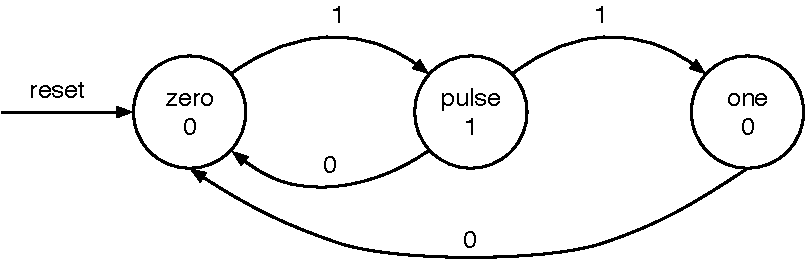
\includegraphics[scale=\scale]{figures/state-diag-rising-moore}
  \caption{The state diagram of the rising edge detector as Moore FSM.}
  \label{fig:diag:rising:moore}
\end{figure}

%\begin{figure}
%  \centering
%  \begin{tikzpicture}[auto,node distance=3cm,
%    thick,main node/.style={circle,draw, minimum size=18pt}, loop/.style={min distance=7mm},>=latex,thick]
%    \coordinate (a);
%    \node [main node, align=center] (b) [right=1.5cm of a,minimum size=1.3cm]{zero\\0};
%    \node [main node, align=center] (c) [right=1.9cm of b,minimum size=1.3cm]{pulse\\1};
%    \node [main node, align=center] (d) [right=1.9cm of c,minimum size=1.3cm]{one\\0};
%
%    \path[->, thick]
%      (a) edge node {reset} (b)
%      (b) edge [bend left] node {1} (c)
%      (c) edge [bend left, above] node {0} (b)
%      (c) edge [bend left] node {1} (d)
%      (d) edge [bend left=45, above] node {0} (b)
%      ;
%  \end{tikzpicture}
%  \caption{The state diagram of the rising edge detector as Moore FSM.}
%  \label{fig:diag:rising:moore}
%\end{figure}

Figure~\ref{fig:diag:rising:moore} shows the state diagram for the rising
edge detection with a Moore FSM. The first thing to notice is that the Moore FSM
needs three states, compared to two states in the Mealy version.
The state \code{pulse} is needed to produce the single-cycle pulse.
The FSM stays in state \code{pulse} just one clock cycle and then
proceeds either back to the start state \code{zero} or to the \code{one}
state, waiting for the input to become 0 again.
We show the input condition on the state transition arrows and the
FSM output within the state representing circles.

\longlist{code/rising_moore_fsm.txt}{Rising edge detection with a Moore FSM.}{lst:fsm:rising:moore}

Listing~\ref{lst:fsm:rising:moore} shows the Moore version of the rising edge detection
circuit. It uses double the number of D flip-flops than the Mealy or directly
coded version. The resulting next state logic is therefore also larger
than the Mealy or directly coded version.

\begin{figure}
  \centering
  \includegraphics[scale=1]{figures/rising}
  \caption{Mealy and a  Moore FSM waveform for rising edge detection.}
  \label{fig:rising}
\end{figure}

Figure~\ref{fig:rising} shows the waveform of a Mealy and a  Moore version
of the rising edge detection FSM. We can see that the Mealy output closely
follows the input rising edge, while the Moore output rises after the clock tick.
We can also see that the Moore output is one clock cycle wide, where the Mealy
output is usually less than a clock cycle.

From the above example, one is tempted to find Mealy FSMs the \emph{better}
FSMs as they need less state (and therefore logic) and react faster than a Moore FSM.
However, the combinational path within a Mealy machine can cause troubles in
larger designs. First, with a chain of communicating FSM (see next chapter), this
combinational path can become lengthy. Second, if the communicating FSMs build
a circle, the result is a combinational loop, which is an error in synchronous design.
Due to a cut in the combinational path with the state register in a Moore FSM,
all the above issues do not exist for communicating Moore FSMs.

In summary, Moore FSMs combine better for communicating state machines; they
are \emph{more robust} than Mealy FSMs. Use Mealy FSMs only when the reaction within the same
clock cycle is of utmost importance. Small circuits such as the rising edge detection,
which are practically Mealy machines, are fine as well.

\section{Exercise}

% This is a boring example, maybe I can find something more interesting
In this chapter, you have seen many examples of very small FSMs.
Now it is time to write some \emph{real} FSM code.
Pick a little bit more complex example and implement the FSM and
write a test bench for it.

A classic example for a FSM is a traffic light controller (see~\cite[Section~14.3]{dally:vhdl:2016}).
A traffic light controller has to ensure that on a switch from red to green
there is a phase in between where both roads in the intersection
have a no-go light (red and orange).
To make this example a little bit more interesting, consider a priority road.
The minor road has two car detectors (on both entries into the intersection).
Switch to green for the minor road only when a car is detected and then switch
back to green for the priority road.

\todo{Luca: Greatest common divisor with Euclide algorithm can be also a nice exercise.
Martin: but this is shown at the Chisel homepage without an FSM.}

\todo{Here a more interesting exercise. And not one from Dally.}

\chapter{Communicating State Machines}
\index{Communicating state machines}

A problem is often too complex to describe it with a single FSM.
In that case, the problem can be divided into two or more smaller and simpler FSMs.
Those FSMs then communicate with signals. One FSM's output is
another FSM's input; one FSM watches the output of the other FSM.
When we split a large FSM into simpler ones, this is called factoring FSMs.
Communicating FSMs are often directly designed from the specification
of the design. A single FSM for the design would be too large in the first place.

\section{A Light Flasher Example}

To discuss communicating FSMs, we use an example
from~\cite[Chapter~17]{dally:vhdl:2016}, the light flasher.
The light flasher has one input \code{start} and one output
\code{light}. The specification of the light flasher is as follows:
\begin{itemize}
\item when \code{start} is high for one clock cycle, the flashing
sequence starts;
\item the sequence is to flash three times;
\item where the \code{light} goes \emph{on} for six clock cycles, and the \code{light} goes \emph{off} for four clock cycles between flashes;
\item after the sequence, the FSM switches the \code{light} \emph{off} and waits
for the next start.
\end{itemize}

The FSM for a direct implementation\footnote{The state diagram is shown
in~\cite[p.~376]{dally:vhdl:2016}.} has 27 states:
one initial state that is waiting for the input, $3 \times 6$ states for the three
\emph{on} states and $2 \times 4$ states for the \emph{off} states.
We do not show the code for this simple-minded implementation of the light
flasher.

The problem can be solved more elegantly by factoring this large FSM into
two smaller FSMs: the master FSM implements the flashing logic, and the timer FSM
implements the waiting. Figure~\ref{fig:flasher} shows the composition of
the two FSMs.

\begin{figure}
  \centering
  \includegraphics[scale=\scale]{figures/flasher}
  \caption{The light flasher split into a Master FSM and a Timer FSM.}
  \label{fig:flasher}
\end{figure}

The timer FSM counts down for 6 or 4 clock cycles to produce the desired timing.
The timer specification is as follows:

\begin{itemize}
\item when \code{timerLoad} is asserted, the timer loads a value into the down counter,
independent of the state;
\item \code{timerSelect} selects between 5 or 3 for the load;
\item \code{timerDone} is asserted when the counter completed the countdown
and remains asserted;
\item otherwise, the timer counts down.
\end{itemize}

\noindent The following code shows the timer FSM of the light flasher:

\shortlist{code/flasher_timer.txt}

\noindent Listing~\ref{lst:flasher:master} shows the master FSM. It has a starting
state \code{off} and states for the complete blinking sequence. In each state it
waits for the time being done. The timer is loaded whenever it is done and in the
initial \code{off} state. Signal \code{timerSelect} selects the value for the \emph{next}
state down counter.

\verylonglist{code/flasher_fsm.txt}{Master FSM of the light flasher.}{lst:flasher:master}

\begin{figure}
  \centering
  \includegraphics[scale=\scale]{figures/flasher2}
  \caption{The light flasher split into a Master FSM, a Timer FSM, and a Counter FSM.}
  \label{fig:flasher2}
\end{figure}

This solution with a master FSM and a timer has still redundancy in the code
of the master FSM. States \code{flash1}, \code{flash2}, and \code{flash3}
are performing the same function, states \code{space1} and \code{space2} as well.
We can factor out the number of remaining flashes into a second counter.
Then the master FSM is reduced to three states: \code{off}, \code{flash},
and \code{space}.

Figure~\ref{fig:flasher2} shows the design with a master FSM and two FSMs
that count: one FSM to count clock cycles for the interval length of \emph{on}
and \emph{off}; the second FSM to count the remaining flashes.
Listing~\ref{lst:counter:fsm} code shows the down counter FSM:

\verylonglist{code/flasher2_counter.txt}{The down counter FSM.}{lst:counter:fsm}


\noindent Note that the counter is loaded with 2 for 3 flashes, as it counts the
\emph{remaining} flashes and is decremented in state \code{space} when the timer
is done. Listing~\ref{lst:flasher2:master} shows the master FSM for the double refactored flasher.

\verylonglist{code/flasher2_fsm.txt}{The master FSM of the double refactored light flasher.}{lst:flasher2:master}

Besides having a master FSM that is reduced to just three states, our current solution
is also better configurable. No FSM needs to be changed if we want to change
the length of the \emph{on} or \emph{off} intervals or the number of flashes.

In this section, we have explored communicating circuits, especially FSMs, that
only exchange control signals. To perform computation we can combine a FSM with
a datapath, as discussed in the next section.

\section{State Machine with Datapath}
\index{State machine with datapath}
\index{FSMD}
\label{sec:fsmd}

One typical example of communicating state machines is a state machine
combined with a datapath. This combination is often called a finite-state machine
with datapath (FSMD). The state machine controls the datapath, and the datapath
performs the computation. The FSM input are the inputs from the environment and the outputs
from the datapath. Some data from the environment is also fed into the datapath, and the
data output comes from the datapath.

\begin{figure}
  \centering
  \includegraphics[scale=\scale]{figures/popcnt-fsmd}
  \caption{A state machine with a datapath.}
  \label{fig:popcnt-fsmd}
\end{figure}

The FSMD shown in Figure~\ref{fig:popcnt-fsmd} serves as an example that computes the
popcount, also called the \myref{https://en.wikipedia.org/wiki/Hamming_weight}{Hamming weight}.
The Hamming weight is the number of symbols different from the zero symbol.
For a binary string, this is the number of `1's.

The popcount unit contains the data input \code{din} and the result output \code{popCount},
both connected to the datapath. For the input and the output we use a ready/valid handshake.
When data is available, valid is asserted. When a receiver can accept data it asserts ready.
When both signals are asserted the transfer takes place. The handshake signals are connected
to the FSM. The FSM is connected with the datapath with control signals towards the datapath
and with status signals from the datapath.
\index{Datapath}

\begin{figure}
  \centering
  \includegraphics[scale=\scale]{figures/popcnt-states}
  \caption{State diagram for the popcount FSM.}
  \label{fig:popcnt-states}
\end{figure}

\begin{figure}
  \centering
  \includegraphics[scale=\scale]{figures/popcnt-data}
  \caption{Datapath for the popcount circuit.}
  \label{fig:popcnt-data}
\end{figure}

We will co-design the FSM and the datapath.
Figure~\ref{fig:popcnt-states} shows the state diagram of the FSM and
Figure~\ref{fig:popcnt-data} shows the datapath for the popcount circuit.
The FSM starts in state \code{Idle}, where the FSM waits for input.
When data arrives, as signaled with an asserted \code{dinValid}, the FSM loads the shift register
and advances to state \code{Count}.
The data is loaded into the \code{shf} register. On the load also the \code{cnt}
register is reset to 0.


In state \code{Count}, the number of `1's is counted sequentially.
We use a shift register, an adder, an accumulator
register, and a down counter (not shown in the datapath) to perform the computation.
To count the number of `1's, the \code{shf} register is shifted
right, and the least significant bit is added to \code{cnt} each clock cycle.
A counter, not shown in the figure, counts down until all bits have been shifted
through the least significant bit.
When the counter reaches zero, the popcount
has finished. The FSM switches to state \code{Done} and signals the result
by asserting \code{popCntReady}. When the result is read, signaled by asserting
\code{popCntValid}, the FSM switches back to \code{Idle},
ready to compute the next popcount.

\longlist{code/popcnt_main.txt}{The top level of the popcount circuit.}{lst:pop:top}

The top level component, shown in Listing~\ref{lst:pop:top}, instantiates the FSM and the datapath
components and connects them.
Listing~\ref{lst:pop:data} shows the Chisel code for the datapath of the popcount
circuit.
On a \code{load} signal, the \code{regData} register is loaded with the input,
the \code{regPopCount} register reset to 0, and the counter register \code{regCount}
set to the number of shifts to be performed.
Otherwise, the \code{regData} register is shifted to the right, the least significant bit
of the \code{regData} register added to the \code{regPopCount} register, and the counter
decremented until it is 0. When the counter is 0, the output contains the popcount.

\verylonglist{code/popcnt_data.txt}{Datapath of the popcount circuit.}{lst:pop:data}
\newpage
\verylonglist{code/popcnt_fsm.txt}{The FSM of the popcount circuit.}{lst:pop:fsm}

Listing~\ref{lst:pop:fsm} shows the code of the FSM.
The FSM starts in state \code{idle}. On a valid signal for the input data (\code{dinValid}) it
switches to the \code{count} state and waits till the datapath has finished counting.
When the popcount is \code{done}, the FSM switches to state \code{done} and waits till the
popcount is read (signaled by \code{popCntReady}).


The popcount example consumed data (a word) and produced data (the popcount).
For the coordinated exchange of data, we use handshake signals.
The next section describes the ready/valid interface for flow control of
unidirectional data exchange.

\section{Ready/Valid Interface}
\index{Ready/valid interface}
\label{sec:ready:valid}

Communication of subsystems can be generalized to the movement
of data and handshaking for flow control. In the popcount example,
we have seen a handshaking interface for the input and for the output data
using valid and ready signals.

\begin{figure}
  \centering
  \includegraphics[scale=\scale]{figures/readyvalid}
  \caption{The ready/valid flow control.}
  \label{fig:readyvalid}
\end{figure}

The ready/valid interface~\cite[p.~480]{dally:vhdl:2016} is a simple flow
control interface consisting of \code{data} and a \code{valid} signal at the
sender side (also called producer or source) and a \code{ready}
signal at the receiver side (also called consumer or destination).
Figure~\ref{fig:readyvalid} shows the ready/valid connection.
The sender asserts \code{valid} when \code{data} is available,
and the receiver asserts \code{ready} when it is ready to receive one word
of data. The transmission of the data happens when both signals, \code{valid}
and \code{ready}, are asserted. If either of the two signals is not asserted,
no transfer takes place.

\begin{figure}
  \centering
  \includegraphics[scale=1]{figures/ready_valid1}
  \caption{Data transfer with a ready/valid interface, early ready.}
  \label{fig:ready_valid1}
\end{figure}

Figure~\ref{fig:ready_valid1} shows a timing diagram of the ready/valid
transaction where the receiver signals \code{ready} (from clock cycle 2 on)
before the sender has data. The data transfer happens in clock cycle 4.
From clock cycle 5 on neither the sender has data nor the receiver is ready
for the next transfer.
When the receiver can receive data in every clock cycle, it is called an
``always ready'' interface and \code{ready} can be hardcoded to \code{true}.

\begin{figure}
  \centering
  \includegraphics[scale=1]{figures/ready_valid2}
  \caption{Data transfer with a ready/valid interface, late ready.}
  \label{fig:ready_valid2}
\end{figure}

Figure~\ref{fig:ready_valid2} shows a timing diagram of the ready/valid
transaction where the sender signals \code{valid} (from clock cycle 2 on)
before the receiver is ready. The data transfer happens in clock cycle 4.
From clock cycle 5 on neither the sender has data nor the receiver is ready
for the next transfer.
Similar to the ``always ready'' interface we can envision and always valid
interface. However, in that case the data will probably not change on signaling
\code{ready} and we would simply drop the handshake signals.

\begin{figure}
  \centering
  \includegraphics[scale=1]{figures/ready_valid3}
  \caption{Single cycle ready/valid and back-to-back transfers.}
  \label{fig:ready_valid3}
\end{figure}

Figure~\ref{fig:ready_valid3} shows further variations of using the the ready/valid
interface. In clock cycle 2 it happens that both signals (\code{ready} and \code{valid})
become asserted just for a single clock cycle and the data transfer
of \code{D1} happens. Data can be transferred back-to-back (in every
clock cycle) as shown in clock cycles 5 and 6 with the transfer of
\code{D2} and \code{D3}

To make this interface composable, neither \code{ready} nor \code{valid} is
allowed to depend combinationally on the other signal.
As this interface is so common, Chisel defines the \code{DecoupledIO}
bundle, similar to the following:

\shortlist{code/fifo_decoupled.txt}

\noindent The \code{DecoupledIO} bundle is parameterized with the type for
the \code{data}. The interface defined by Chisel uses the field \code{bits}
for the data. \code{DecoupledIO} is part of the package \code{chisel3.util}.

One question remains if the \code{ready} or \code{valid} may be deasserted
after being asserted and \emph{no} data transfer has happened.
For example a receiver might be ready for some time and not receiving data, but
due to some other events may become not ready.
The same can be envisioned with the sender, having data valid only some
clock cycles and becoming non-valid without a data transfer happened.
If this behavior is allowed or not is not part of the ready/valid interface,
but needs to be defined by the concrete usage of the interface.

Chisel places no requirements on the signaling of \code{ready} and \code{valid}
when using the class \code{DecoupledIO}.
However, the class \code{IrrevocableIO} places following restrictions
on the sender:

\begin{quote}
A concrete subclass of \code{ReadyValidIO} that promises to not change
the value of \code{bits} after a cycle where \code{valid} is high and \code{ready} is low.
Additionally, once \code{valid} is raised it will never be lowered until after
\code{ready} has also been raised.
\end{quote}

\noindent Note that this is \emph{just} a convention that cannot be enforced \emph{just}
by using the class \code{IrrevocableIO}.

The AXI  bus~\cite{axi4standard} uses one ready/valid interface for each of the following parts of the bus:
read address, read data, write address, and write data. AXI restricts the interface
that once the sender assets \code{valid} it is not allowed to deasserted it
until the data transfer happened. This is the same restriction as just described
in the comment of the \code{IrrevocableIO} interface.
Furthermore, the sender is not allowed to wait for a receivers
\code{ready} to assert \code{valid}.
The receiver side is more relaxed. If \code{ready} is asserted, it is allowed to deassert it
before \code{valid} is asserted. Furthermore, the receiver is allowed to wait for a asserted
\code{valid} before asserting \code{ready}.

\longlist{code/ready_valid_buffer.txt}{A register as a buffer with a ready/valid interface}{lst:rv:reg}

Listing~\ref{lst:rv:reg} shows an example of using the ready/valid interface.
The circuit represents a buffer built out of a register.
The buffer has a ready/valid interface (\code{DecoupledIO}) at the input and one at the output.
The \code{DecoupledIO} bundle is defined from the sender's viewpoint. Therefore,
the input of the buffer (\code{in}) needs to change the direction with \code{Flipped}.

The module contains a register for the data (\code{dataReg}) and a single bit
register (\code{emptyReg}) signaling if the buffer is empty or full.
This single bit represents a two state Moore FSM with states empty and full.
The input \code{ready} signal and the output \code{valid} signal depend only
on the state of \code{emptyReg}. There is no combinational path between the
input and the output of the buffer.

When the buffer is empty and there is valid data at the input, the data is registered
and the state changed to full. When the buffer is full and the consumer side signals
to be ready, the data is considered read and the buffer is empty again.



\chapter{Hardware Generators}
\index{Hardware generators}
\label{ch:gen}

The strength of Chisel is that it allows us to write hardware generators.
With older hardware description languages, such as VHDL and Verilog,
we usually use another language, for example, Java or Python, to generate hardware.
Before using Chisel, I have often written small Java programs to generate VHDL tables.
In Chisel, the full power of Scala and Java with its many open-source libraries
are available at hardware construction time. Therefore, we can write our hardware
generators in the same language and execute them as part of the Chisel circuit generation.

\section{A Little Bit of Scala}
\index{Scala}

This subsection gives a very brief introduction into Scala. It should be enough
to write simple hardware generators for Chisel.
For an in-depth introduction into Scala I recommend the textbook by Odersky et al.~\cite{Scala}.
The \myref{https://www.scala-lang.org/}{Scala website} also contains an
\myref{https://docs.scala-lang.org/overviews/scala-book/introduction.html}{online Scala book}.\footnote{The link
points to the Scala 2 version of the book, as Chisel is still based on Scala 2.}

Scala has two types of variables: \code{val}s and \code{var}s. A \code{val} gives an expression
a name and cannot be reassigned a value. This following snippet shows the definition of
an integer value called \code{zero}. If we try to reassign a value to \code{zero}, we get
a compile error.

\shortlist{code/scala_val.txt}
\index{Scala!val}

\noindent In Chisel we use \code{val}s to name hardware components. Note that the \code{:=}
operator is a Chisel operator and not a Scala operator.

Scala also provides the more classic version of a mutable variable as \code{var}. The following code defines
an integer variable and reassigns it a new value:

\shortlist{code/scala_var.txt}

\noindent We will need Scala \code{var}s to write hardware \emph{generators}, but never need
\code{var}s to name a hardware \emph{component}.

You may have wondered what type those variables have. As we assigned an integer constant
in the above example, the type of the variable is \emph{inferred}; it is a Scala \code{Int} type.
In most cases the Scala compiler is able to infer the type. However, if we are in the mood of
being more explicit, we can explicitly state the type as follows:

\shortlist{code/scala_int_type.txt}

Simple loops are written as follows:

\shortlist{code/scala_loop.txt}
\index{Scala!for loop}

We use a loop for circuit generators. The following loop connects individual bits
of a shift register.

\shortlist{code/scala_loop_gen.txt}

\noindent Note that this is not the most concise expression of a shift register.
It is better to use a plain \code{UInt} with the right size and assign the new value for the
register with an expression using the \code{\#\#} operator
and proper indexing. This code snippet is just to show how a Scala \code{for} loop can be used
for circuit generation.

Conditions are expressed with \code{if} and \code{else}. Note that this condition
is evaluated at Scala runtime during circuit generation. This construct does \emph{not}
create a multiplexer, but allows to write \emph{configurable} hardware generators.

\shortlist{code/scala_condition.txt}

Scala has the notion of a \myref{https://en.wikibooks.org/wiki/Scala/Tuples}{tuple}.
A tuple can hold a sequence of different types. The tuple is built by placing the individual fields
within parentheses. The fields are then accessed with \code{.\_n}, starting with 1 for the first field.
Following code creates a tuple to represent a city with the zip code and the name.

\index{Scala!tuple}

\shortlist{code/scala_tuple.txt}

\noindent Tuples are useful when we want to return more than one value from a function.
Tuples allow us to represent Chisel components with more than one output as a lightweight
function instead of a full-blown module.

Scala has a powerful \myref{https://docs.scala-lang.org/overviews/collections-2.13/overview.html}{collection library}.
One of the simpler collection types is \code{Seq}, an ordered collection of elements (also called a sequence).
The default implementation is immutable. We index into a \code{Seq} with \code{()},
with zero-based indexing.
\code{Seq} is a base class with several different implementations.
However, for most Chisel hardware generators direct use of \code{Seq}
is the preferred choice. The following code shows how to create a \code{Seq}
that holds four Scala \code{Int} values. The second line accesses the
second element, and \code{second} will be \code{15}.

\index{Scala!Seq}


\shortlist{code/scala_seq.txt}



\section{Lightweight Components with Functions}
\label{sec:functions}

\index{Function components}

Modules are the standard way to structure your hardware description.
However, there is some boilerplate code when declaring a module and when instantiating and
connecting it.
A lightweight way to structure your hardware is to use functions.
Scala functions can take Chisel (and Scala) parameters and return generated hardware.
As a simple example, we generate an adder:

\shortlist{code/components_fn_def.txt}

\noindent The return value of a function in Scala is the result of the last
expression.\footnote{Scala also contains a \codefoot{return} statement. The code could have been written
a bit more verbose as \codefoot{return x + y}.}
We can then create two adders by simply calling the function \code{adder}.

\shortlist{code/components_fn_use.txt}

\noindent Note that this is a \emph{hardware generator}. That code is not executing any add operation
during elaboration, but creates two adders (hardware instances). Or in other words, it returns
a wire to the output of the adder.
We have written our first hardware generator!

The adder is an artificial example
to keep it simple. Chisel has already an adder generator function, like \code{+(that: UInt)}.

Functions, as lightweight hardware generators, can also contain state (using a register).
The following example returns a one clock cycle delay element (a register).
If a function has just a single statement, we can write it in one line and omit the curly
braces (\{\}).

\shortlist{code/components_fn_delay.txt}

\noindent By calling the function with the function itself as parameter, this generated a two
clock cycle delay.

\shortlist{code/components_fn_2delay.txt}

\noindent Again, this is too short an example to be useful, as \code{RegNext()}
is already that function that creates the register for the delay.



Functions return only one value. In order to provide more than one output, we
can wrap several output wires into a Scala tuple. The following code generates hardware that
compares two inputs and has two outputs.

\shortlist{code/fun_comp.txt}

\noindent With the parenthesis, we wrap the two wires that are connected to the outputs of
the comparator circuit into a Scala tuple.

When creating a comparator component
with the \code{compare} function, it returns a tuple of two wires. We can access the two
wires with the \code{.\_n} syntax.

\shortlist{code/fun_comp_use1.txt}

\noindent However, we can directly decompose the tuple into two wires, in this case \code{equ}
and \code{gt}, with following syntax.

\shortlist{code/fun_comp_use2.txt}


Functions can be declared as part of a \code{Module}. However, functions that will be
used in different modules are better placed into a Scala object that collects utility
functions.

\section{Generate Combinational Logic}
\index{Logic generation}
\index{Logic table generation}
\index{ROM}
\label{sec:gen:comb:logic}

A logic table (truth table) is combinational logic. It is also called read-only memory (ROM),
as we can see the input to the table as an address into such a ROM.
We generate a logic table with \code{VecInit}.  The following snippet of code creates
a table to compute the square of a number \code{n}.

\shortlist{code/gen_vec.txt}

We can use the full power of Scala to generate our logic (tables).
For example, we can generate a table of fixpoint constants to represent a trigonometric function,
compute constants for digital filters, or write an assembler in Scala
to generate code for a microprocessor written in Chisel. All those functions
are in the same code base (same language) and can be executed during
hardware generation.

\index{Binary-coded decimal}
\index{BCD}
A classic example for a table generation is the conversion of a binary number
into a \myref{https://en.wikipedia.org/wiki/Binary-coded_decimal}{binary-coded decimal}
(BCD) representation. BCD is used to represent a number in a decimal
format using 4 bits for each decimal digit. For example, decimal \code{13} is in binary
\code{1101} and BCD encoded as 1 and 3 in binary: \code{00010011}.
BCD allows displaying numbers in decimal, a more user-friendly number
representation than hexadecimal.

When using a classic hardware description language, such as Verilog or VHDL,
we would use another scripting or programming language to generate such a table.
We can write a Java program that computes the table to convert binary to BCD.
That Java program prints out VHDL code that can be included in a project.
The Java program is about 100 lines of code; most of the code generating
VHDL strings. However, the key part of the conversion is just two lines of code.
With Chisel, we can compute this table directly as part of the hardware generation.
Listing~\ref{lst:bcd} shows the table generation for the binary to BCD conversion.

\longlist{code/bcd_table.txt}{Binary to binary-coded decimal conversion.}{lst:bcd}

\subsection{File Reading}
\index{File reading}

\longlist{code/file_reader.txt}{Reading a text file to generate a logic table.}{lst:file:reader}

We can also generate a logic table from a Scala \code{Array}.
We may have data in a file that we want to read in during hardware generation
time for the logic table.
Listing~\ref{lst:file:reader} shows how to use the Scala \code{Source}
class form the Scala standard library to read the file \code{data.txt}, which
contains integer constants in a textual representation.\footnote{Scala is
based on Java and therefore all Java file reading and writing libraries can
be used, e.g., to read binary files.}
\index{VecInit}

A few words on the maybe a bit intimidating expression:
\begin{chisel}
  val table = VecInit(array.toIndexedSeq.map(_.U(8.W)))
\end{chisel}


\noindent The method \code{toIndexedSeq} converts a Scala \code{Array}
to a Scala sequence (\code{Seq}),
which supports the mapping function \code{map}.
\code{map} invokes a function on each element of the sequence and returns
a sequence of the return value of the function. Our function \code{\_.U(8.W)} represents
each \code{Int} value from the Scala array as a \code{\_} and performs the conversion
from a Scala \code{Int} value to a Chisel \code{UInt} literal, with a size of 8 bits.
The Chisel object \code{VecInit} creates a Chisel \code{Vec} from a sequence \code{Seq}
of Chisel types.

We can use the initialization of a Chisel \code{Vec} from a Scala sequence to represent
a message that we may send out to a serial port.
A Scala/Java \code{String} is a Scala \code{Seq}.
Therefore, the \code{map}
method is available to map each Scala \code{Char} to a Chisel \code{UInt}.
The following code converts the standard greeting
from the \code{msg} string to a Chisel \code{Vec}:

\shortlist{code/hello_table.txt}

\noindent This code is extracted from the serial port example, which is used later in this text to send a welcome message.

\subsection{Type Conversion}
\index{Type!conversion}

Sometimes it is convenient to convert from one Chisel type to a different type.
All types basically represent a collection of bits. Therefore, we can easily preform this mapping.
As a first example let us assume we receive bytes of data and would like to repackage
4 bytes into a 32-bit \code{UInt}. Following code maps the vector of bytes to an \code{UInt}.
The bytes are mapped in following order to the \code{UInt}: the first byte into the lower 8 bits,
the next byte into the next and so on.

\shortlist{code/convert_vec2uint.txt}

\noindent Given a \code{UInt} \code{word}, we can convert it back to a vector
of four bytes.

\shortlist{code/convert_uint2vec.txt}

We can also convert a \code{Bundle} to a \code{UInt}. The bundle fields are ordered
that the last field (in this example field \code{b}) is in the lower bits of the \code{UInt}
(here 15 to 0), folloed by the second last, and so on. Note, that this order is opposite to
the order of mapping a \code{Vec}.

\shortlist{code/convert_bundle2uint.txt}

\noindent A \code{UInt} can be converted (back) to a bundle as follows:

\shortlist{code/convert_uint2bundle.txt}

\noindent That conversion can also be used to initialize all fields of a bundle to 0.

\shortlist{code/convert_zero2bundle.txt}


\section{Configuration with Parameters}
\index{Parameters}

Chisel components and functions can be configured with parameters.
Parameters can be as simple as an integer constant, but can also be a Chisel
hardware type.

\subsection{Simple Parameters}

The simplest way to parameterize a circuit is to define a bit width as a parameter.
Parameters can be passed as arguments to
the constructor of the Chisel module. The following example is a toy example of
a module that implements an adder with a configurable bit width.
The bit width \code{n} is a parameter (of Scala type \code{Int}) of the component
passed into the constructor that can be used in the IO bundle.

\shortlist{code/param_adder.txt}

\noindent Parameterized versions of the adder can be created as follows:

\shortlist{code/use_param_adder.txt}

\subsection{Case Classes}
\index{Case classes}

If we need more parameters, we can simply add additional parameters to the constructor
of the Chisel module. However, if we pass those parameters through several constructors
it might become tedious to use them. Furthermore, when changing the number or type of
parameters, we need to edit several places.

Scala has a very light-weight construct to package several fields into a class:
a \myref{https://docs.scala-lang.org/tour/case-classes.html}{case classes}.
Case classes are like regular Scala classes, but with a very light-weight definition.
Following code defines a case class to represent three parameters. It might be used for
a device with a transmit (tx) buffer and a receive buffer(rx) of a certain width.

\shortlist{code/case_class.txt}

\noindent An object of that case class is created by simply calling the constructor.
The fields are immutable and can be read by accessing them:

\shortlist{code/case_class_use.txt}

\noindent We can also add code to the case class to check that the parameters
are valid.

\shortlist{code/case_class_save.txt}

\subsection{Functions with Type Parameters}
\index{Type!parameters}

Having the bit width as a configuration parameter is just the starting point for
hardware generators. Chisel type parameters enable very flexible configurations.
That feature allows for Chisel to provide a multiplexer (\code{Mux}) that
can accept any types for the multiplexing.
To show how to use Chisel types for the configuration, we build a multiplexer
that accepts arbitrary types. The following function defines the multiplexer:

\shortlist{code/param_func.txt}

Chisel allows parameterizing functions with types, in our case with Chisel
types. The expression in the square brackets \code{[T <: Data]} defines
a type parameter \code{T} that is \code{Data} or a subclass of \code{Data}.
\code{Data} is the root of the Chisel type system.

Our multiplexer function has three parameters: the boolean condition,
one parameter for the true path, and one parameter for the false path.
Both path parameters are of type \code{T}, which is
provided at function call. The function itself is straightforward:
we define a wire with the default value of \code{fPath} and
change the value if the condition is true to the \code{tPath}.
This condition is a classic multiplexer function.
At the end of the function, we return the multiplexer hardware (the output).
We can use our multiplexer function with simple types such as
\code{UInt}:

\shortlist{code/param_func_simple.txt}

\noindent The types of the two multiplexer paths need to be the same.
The following wrong usage of the multiplexer results in a runtime error:

\shortlist{code/param_func_wrong.txt}

\noindent To show a more complex multiplexer, we define a new type as a \code{Bundle} with two fields:

\shortlist{code/param_func_type.txt}

\noindent We can define \code{Bundle} constants by first creating
a \code{Wire} of the \code{Bundle} and then setting the subfields.
Then we can use our parameterized multiplexer with this complex type.

\shortlist{code/param_func_complex.txt}

In our initial design of the function, we used \code{WireDefault}
to create a wire with the type \code{T} with a default value.
If we need to create a wire just of the Chisel type without using a default
value, we can use \code{fPath.cloneType} to get the Chisel type.
The following function shows the alternative way to code the multiplexer.

\shortlist{code/param_func_alt.txt}

\subsection{Modules with Type Parameters}

We can also parameterize modules with Chisel types.
Let us assume we want to design a network-on-chip to move data between
different processing cores. However, we do not want to hardcode the
data format in the router interface; we want to \emph{parameterize} it.
Similar to the type parameter for a function, we add a type parameter \code{T}
to the Module constructor. Furthermore, we need to have one constructor
parameter of that type. Additionally, in this example, we also make the number
of router ports configurable.

\shortlist{code/param_mod.txt}

\noindent To use our router, we first need to define the data type we want to route, e.g.,
as a Chisel \code{Bundle}:

\shortlist{code/param_mod_type.txt}

\noindent We create a router by passing an instance of the user-defined Bundle and
the number of ports to the constructor of the router:

\shortlist{code/param_mod_use.txt}

\subsection{Parameterized Bundles}

In the router example, we used two different vectors of fields for the input
of the router: one for the address and one for the data, which was parameterized.
A more elegant solution would be to have a \code{Bundle} that itself
is parametrized. Something like:

\shortlist{code/param_bundle_issue.txt}

The \code{Bundle} has a parameter of type \code{T}, which is a subtype
of Chisel's \code{Data} type.
Within the bundle, we define a field \code{data} by invoking \code{cloneType}
on the parameter.
However, when we use a constructor parameter, this parameter becomes a
public field of the class. When Chisel needs to clone the type of the \code{Bundle},
e.g., when it is used in a \code{Vec}, this public field is in the way.
A solution (workaround) to this issue is to make the parameter field private:

\shortlist{code/param_bundle.txt}

\noindent With that new \code{Bundle}, we can define our router ports

\shortlist{code/param_mod2.txt}

\noindent and instantiate that router with a \code{Port} that takes
a \code{Payload} as a parameter:

\shortlist{code/param_mod_use2.txt}

\subsection{Optional Ports}

Some hardware generator might have IO ports that are dependent on a configuration.
As an example we implement a register file for typical 32-bit RISC processor. For debugging
we want to be able to access all register. Therefore, we want to have an additional
port where we can read all registers in the tester. However, at Verilog generation
we do not want this expensive extra port.

Listing~\ref{lst:reg:file} shows such a register file. It has as parameter \code{debug}
as a Scala \code{Boolean}. In the definition of the IO bundle we use that parameter
to either generate that port or not. In Scala this is represented as an \code{Option}.
An option can return a value wrapped into \code{Some} or represent the missing value
as a \code{None}. In the main body of the module we extract the value of the option
with \code{get}.

\longlist{code/register_file.txt}{A register file with an optional debug port.}{lst:reg:file}

Similar in the tester we need to  use options \code{get} method to get a reference
of that IO port:

\shortlist{code/register_file_test.txt}


\section{Use Inheritance}
\label{sec:inheritance}

\index{Inheritance}
\index{Object-oriented}

Chisel is an object-oriented language. A hardware component, the Chisel \code{Module},
is a Scala class. Therefore, we can use inheritance to factor a common behavior
out into a parent class. We explore how to use inheritance with an example.

In Section~\ref{sec:counter} we have explored different forms of counters,
which may be used for a low-frequency tick generation. Let us assume we want to
explore those different versions, for example, to compare their resource requirement.
We start with an abstract class to define the ticking interface, shown in Listing~\ref{lst:ticker:base}.

\longlist{code/ticker.txt}{Base class for our ticker implementations.}{lst:ticker:base}

\noindent Listing~\ref{lst:ticker:up} shows a first implementation of that abstract class
with a counter, counting up, for the tick generation.

\longlist{code/up_ticker.txt}{Tick generation with a counter.}{lst:ticker:up}

We can test all different versions of our \emph{ticker} logic with a single test bench.
We \emph{just} need to define the test bench to accept subtypes of \code{Ticker}.
Listing~\ref{lst:ticker:test} shows the Chisel code for the tester.
The \code{TickerTester} has several parameters: (1) the type parameter
\code{[T <: Ticker]} to accept a \code{Ticker} or any class that inherits from \code{Ticker},
(2) the design under test, being of type \code{T} or a subtype thereof,
and (3) the number of clock cycles we expect for each tick.
The tester waits for the first occurrence of a tick (the start might be different for
different implementations) and then checks that \code{tick} repeats every $n$ clock cycles.

\longlist{code/ticker_tester.txt}{A tester for different versions of the ticker.}{lst:ticker:test}

With a first, easy implementation of the ticker, we can test the tester
itself, probably with some \code{println} debugging. When we are confident that
the simple ticker and the tester are correct, we can proceed and explore
two more versions of the ticker. Listing~\ref{lst:ticker:down} shows the tick
generation with a counter counting down to 0.
Listing~\ref{lst:ticker:nerd} shows the nerd version of counting down to -1 to use
less hardware by avoiding the comparator.

\longlist{code/down_ticker.txt}{Tick generation with a down counter.}{lst:ticker:down}

\longlist{code/nerd_ticker.txt}{Tick generation by counting down to -1.}{lst:ticker:nerd}

We can test all three versions of the ticker by using ScalaTest specifications,
creating instances of the different versions of the ticker and passing them
to the generic test bench. Listing~\ref{lst:ticker:spec} shows the test specification.
We run only the ticker tests with:
\begin{chisel}
sbt "testOnly TickerTest"
\end{chisel}

\longlist{code/ticker_test.txt}{ChiselTest for the ticker tests.}{lst:ticker:spec}

\section{Hardware Generation with Functional Programming}
\label{sec:functional}

\index{Functional programming}

Scala supports functional programming, so Chisel does as well.
We can use functions to represent hardware and combine those hardware components
with functional programming by using a ``higher-order function''.
Let us start with a simple example, the sum of a vector:

\shortlist{code/fun_first.txt}

First we define the hardware for the adder in function \code{add}.
The vector (Chisel type \code{Vec}) is located in \code{vec}. The Scala method \code{reduce()} combines
all elements of a collection with a binary operation, producing a single value.
The \code{reduce()} method reduces the sequence starting from the first element.
It takes the first two elements and performs the operation. The result is then combined
with the next element, until a single result is left.

The function to combine two elements is provided as parameter to \code{reduce}, in our case \code{add},
which returns an adder. The resulting hardware is a chain of adders computing
the sum of the elements of vector \code{vec}.
Instead of defining the (simple) \code{add} function, we can provide the addition
as anonymous function and use the Scala wildcard ``\code{\_}'' to represent the
two operands.

\shortlist{code/fun_func_lit.txt}

\noindent With this one-liner we have generated the chain of adders. For the sum function
a chain is not the ideal configuration; a tree will have a shorter combinational delay.
If we do not trust the synthesize tool to rearrange our adder chain, we can use Chisel's
\code{reduceTree} method to generated a tree of adders:

\shortlist{code/fun_reduce_tree.txt}

\subsection{Minimum Search Example}

As a more elaborate example, we will build a circuit to find the minimum value in a \code{Vec}. To express this circuit
we use an anonymous function, called \emph{function literal} in Scala.  The syntax for a function
literal is parameters in parentheses, followed by a \code{=>}, followed by the function body:

\begin{chisel}
  (param) => function body
\end{chisel}

The function literal for the minimum function uses two parameters \code{x} and \code{y}
and returns a multiplexer (\code{Mux}) that compares the two parameters and returns the smaller
value.

\shortlist{code/fun_min.txt}

Let us extend this circuit to return not only the minimal value from the \code{vec}, but also the
position (index) of that minimal value in the \code{vec}. To return two values we define the Bundle \code{Two} to
hold the value and the index. We declare the \code{vecTwo} \code{Vec} that can hold these bundles
and connect them in a loop to the original input and the index within the \code{Vec}, as shown
in Listing~\ref{lst:min:pos}.

As before, we use a function literal in the \code{reduceTree} method of the \code{vecTwo},
comparing the value field within the bundle and returning the multiplexer for the
complete bundle.
Value \code{res} points to the bundle containing the minimum value and the position.

\longlist{code/fun_min2.txt}{Minimum search including the index.}{lst:min:pos}


As a more advanced variation of the minimum search circuit, we will use more Scala features
to avoid creating the bundle to return the value
and index. We will use a tuple to represent both values.
The following code shows the application
of a chain of functions to the original sequence. Chaining functions is a typical pattern in functional programming.
This pattern can also be seen as a pipeline of operations.

\shortlist{code/fun_min3.txt}

The first function (\code{zipWithIndex})
transforms the original sequence of \code{UInt}s to a sequence of tuples, where the first element is the
unchanged \code{UInt} and the second element is the index value within the \code{vec} as Scala \code{Int}.
In general a \code{zip} function merges two sequences (zips them) into a single one
containing the two elements as tuples.

% fixme: the following two sentences are unclear.
% "provides the generation of the minimum finding" in particular is cryptic.
The next function maps our tuple of a Chisel \code{UInt}
and a Scala \code{Int} to two Chisel \code{UInt}s. The \code{reduce} function provides the generation of
the minimum finding. We compare the first element of the tuple in two multiplexers and return
a tuple containing the minimum value and the position as Chisel \code{UInt} types.


Note that the whole functional expression uses a Scala \code{Vector} to hold intermediate results,
but returns hardware (connected multiplexers) consisting of Chisel types only.
As we use a Scala \code{Vector} here, we cannot use \code{reduceTree}, which is available on Chisel's
\code{Vec} only.

To keep using \code{reduceTree} the following solution uses a Chisel \code{MixedVec}
instead of a Scala tuple.
A Chisel \code{MixedVec} is similar to a Scala tuple as it can have different types at different positions.
Therefore, it cannot function as, for example, multiplexer. However, we can use it as an
indexable collection during hardware generation.

\shortlist{code/fun_min4.txt}


In the above example we create a Scala \code{Vector} of the values with their index, but now
using Chisel's ``tuple''. We then convert the Scala \code{Vector} into a Chisel \code{Vec}.
Then we can again perform a tree-based reduction. Another benefit of this version is
that we have only one multiplexer, which selects between two Chisel ``tuples'' that are actually
\code{MixedVec}s.
The result in \code{resFun2} is a \code{MixedVec} with two elements,
accessed with an index, like a ``normal'' \code{Vec}.

\subsection{An Arbitration Tree}
\index{Arbiter}
\label{sec:arbiter}

With our tree reduction function we can build an arbitration tree out of just 2:1 arbiters.
We can generate the arbitration circuit as follows:

\shortlist{code/fun_arbiter_head.txt}
\shortlist{code/fun_arbiter_end.txt}

\noindent The input is a \code{Vec} of ready/valid interfaces and the output a single ready/valid
interface. We \emph{just} need a function that provides arbitration between two requests.



\subsubsection{Simple Arbitration}

As a first solution, we will build a priority-based arbitration, similar to the arbiter shown
in Section~\ref{sec:arbiter}. That arbiter in Section~\ref{sec:arbiter} was a purely combinational circuit.
However, with the ready/valid interface we are not allowed to have a combinational
flow between a ready and a valid signal. Therefore, we need to introduce state for those signals
and also need to register the incoming data.

Listing~\ref{lst:fun:arbiter:simp} shows the 2-to-1 arbitration function. This function assumes
that a requester who has asserted \code{valid} will only deassert it when it is read by the receiver
(signaled with a \code{ready}). Furthermore, we are allowed to set \code{ready} in the next clock cycle
depending on \code{valid} in the current clock cycle.
This is one specific interpretation of the ready/valid protocol, which is also used in AXI.

\longlist{code/fun_arbiter_simple.txt}{A simple 2 to 1 arbiter.}{lst:fun:arbiter:simp}

We need the following registers: \code{regData} to hold the data for the output, \code{regEmpty} as a  flag to
signal that the data register is empty, and two flags for the \code{ready} signals of the two inputs
(\code{regReadyA} and \code{regReadyB}).
The return value of the function (\code{out}) is a wire of type \code{DecoupledIO}.

When the data register is empty and one of the two inputs signals a \code{valid} input,
we signal a \code{ready} in the next clock cycle (via the \code{ready} register).
Note that we can signal only one of the two inputs that the arbiter is \code{ready},
as we have only one data register.
When we have a registered \code{ready}, we assume that the input is still \code{valid},
register the data, deassert \code{regEmpty}, and reset the \code{ready} flag.

The output is valid, when the data register is not empty. When the receiver is \code{ready},
the data is transmitted and the data register is empty again.
As the last statement, the function returns \code{out}, the reference to the \code{DecoupledIO}
wire.


\subsubsection{Fair Arbitration}

In Section~\ref{sec:arbiter} we presented a combinational version of an arbitration circuit.
The combinational version is a priority arbiter, so one high-priority requester can
dominate the arbitration.
To avoid this domination, we need to introduce state to remember who won the arbitration last time.
Our assumption is that if the 2:1 arbiter is fair, this results in a fair
arbitration on a balanced arbitration tree.

\longlist{code/fun_arbiter.txt}{A fair 2-to-1 arbiter.}{lst:fun:arbiter}

Listing~\ref{lst:fun:arbiter} shows that fair 2:1 arbitration circuit.
The arbiter contains one register for the data to store and one state register. To be fair, the arbiter
switches between two idle states (\code{idleA} and \code{idleB}) when there is no request.
In each of the two idle states it accepts only one of the inputs. Note that with just a single register for
storage, the arbiter can only be ready for one of the two inputs. To allow being ready for both inputs
and switching priority we would need a second data register to handle the case when both inputs
are valid in the same clock cycle.

When a request is accepted, it stores the data and switches to one of the full states (\code{hasA}
or \code{hasB}).
When the consumer of the output accepts the data, the arbiter switches back to an idle state.
It switches to the idle state that will accept a pending request from the other input
in the next clock cycle.



\chapter{Example Designs}

In this section, we explore some small digital designs, such as
a FIFO buffer, which are used as building blocks for a larger design.
As another example, we design a serial interface (also called UART),
which itself may use the FIFO buffer. Furthermore, we will generalize
the FIFO interface and show different possible implementations.

\section{FIFO Buffer}
\label{sec:fifo}

\index{FIFO}
\index{FIFO buffer}
\index{First-in, first-out buffer}


We can decouple a writer (sender) and a reader (receiver) by a buffer
between the writer and reader.
A common buffer is a first-in, first-out
(\href{https://en.wikipedia.org/wiki/FIFO_%28computing_and_electronics%29}{FIFO})
buffer. Figure~\ref{fig:fifo} shows a writer, the FIFO, and a reader.
Data is put into the FIFO by the writer on \code{din} with an active
\code{write} signal. Data is read from the the FIFO by the reader on
\code{dout} with an active \code{read} signal.

\begin{figure}
  \centering
  \includegraphics[scale=\scale]{figures/fifo}
  \caption{A writer, a FIFO buffer, and a reader.}
  \label{fig:fifo}
\end{figure}

A FIFO is initially empty, singled by the \code{empty} signal. Reading
from an empty FIFO is usually undefined. When data is written and never
read a FIFO will become \code{full}. Writing to a full FIFO is usually ignored
and the data are lost. In other words, the signals \code{empty} and \code{full}
serve as handshake signals

Several different implementations of a FIFO are possible: For example, using on-chip
memory and read and write pointers or simply a chain of registers with a
tiny state machine. For small buffers (up to tens of elements) a FIFO organized
with individual registers connected into a chain of buffers is a simple
implementation with a low resource requirement.
The code of the bubble FIFO is available in the
\myref{https://github.com/schoeberl/chisel-examples}{chisel-examples}
repository.\footnote{For completeness, the Chisel book repository contains
a copy of the FIFO code as well.}

We start by defining the IO signals for the writer and the reader side.
The size of the data is configurable with \code{size}.
The write data are \code{din} and a write is signaled by \code{write}.
The signal \code{full} performs the
\myref{https://en.wikipedia.org/wiki/Flow_control_(data)}{flow control}
at the writer side.

\shortlist{code/bubble_fifo_writer_io.txt}

The reader side provides data with \code{dout} and the read is initiated
with \code{read}. The \code{empty} signal is responsible for the flow control
at the reader side.

\shortlist{code/bubble_fifo_reader_io.txt}

Listing~\ref{lst:fifo:stage} shows a single buffer. The buffer has a enqueueing port
\code{enq} of type \code{WriterIO} and a dequeueing port \code{deq} of type
\code{ReaderIO}. The state elements of the buffer is one register that holds the
data (\code{dataReg}) and one state register for the simple FSM (\code{stateReg}).
The FSM has only two states: either the buffer is \code{empty} or \code{full}.
If the buffer is \code{empty}, a write will register the input data and change
to the \code{full} state.
If the buffer is \code{full}, a read will consume the data and change to the
\code{empty} state.
The IO ports \code{full} and \code{empty} represent the buffer state for
the writer and the reader.

\longlist{code/bubble_fifo_register.txt}{A single stage of the bubble FIFO.}{lst:fifo:stage}

\index{Bubble FIFO}
Listing~\ref{lst:fifo} shows the complete FIFO. The complete FIFO has
the same IO interface as the individual FIFO buffers.
\code{BubbleFifo} has as parameters the \code{size} of the data
word and \code{depth} for the number of buffer stages.
We can build a \code{depth} stages bubble FIFO out of \code{depth}
\code{FifoRegister}s. We create the stages by filling them into a Scala \code{Array}.
The Scala array has no hardware meaning, it \emph{just} serves as
a container to have references to the created buffers.
In a Scala \code{for} loop we connect the individual buffers.
The first buffer's enqueueing side is connected to the enqueueing IO of
the complete FIFO and the last buffer's dequeueing side to the
dequeueing side of the complete FIFO.

\longlist{code/bubble_fifo.txt}{A FIFO is composed of an array of FIFO bubble stages.}{lst:fifo}

The presented idea of connecting individual buffers to implement a FIFO
queue is called a bubble FIFO, as the data bubbles through the queue.
This is simple, and a good solution when the data rate is considerable slower
than the clock rate, for example, as a decouple buffer for a serial port, which is presented
in the next section.

However, when the data rate approaches the clock frequency, the bubble FIFO
has two limitations: (1) As each buffer's state has to toggle between \emph{empty} and
\emph{full}, which means the maximum throughput of the FIFO is 2 clock cycles
per word. (2) The data needs to bubble through the complete FIFO, therefore,
the latency from the input to the output is at least the number of buffers.
I will present other possible implementations of FIFOs in Section~\ref{sec:more:fifo}.

\section{A Serial Port}
\label{sec:uart}
\index{Serial port}
\index{UART}

A serial port (also called
\myref{https://en.wikipedia.org/wiki/Universal_asynchronous_receiver-transmitter}{UART}
or \myref{https://en.wikipedia.org/wiki/RS-232}{RS-232}) is one of the easiest options
to communicate between your laptop and an FPGA board.
As the name implies, data is transmitted serially. An 8-bit byte is transmitted as follows:
one start bit (0), the 8-bit data, least significant bit first, and then one or two stop
bits (1). When no data is transmitted, the output is 1.
Figure~\ref{fig:uart:wave} shows the timing diagram of one byte transmitted.

\begin{figure}
  \centering
  \includegraphics[scale=1]{figures/uart_wave}
  \caption{One byte transmitted by a UART.}
  \label{fig:uart:wave}
\end{figure}

We design our UART in a modular way with minimal functionality
per module. We present a transmitter (TX), a receiver (RX),
a buffer, and then usage of those base components.

First, we need an interface, a port definition.
For the UART design, we use a ready/valid handshake interface (extending \code{DecoupledIO}),
with a data size of 8 bits.
\shortlist{code/uart_channel.txt}
\noindent The convention of a ready/valid interface is that the data is transferred
when both \code{ready} and \code{valid} are asserted.

\longlist{code/uart_tx.txt}{A transmitter for a serial port.}{lst:uart:tx}

Listing~\ref{lst:uart:tx} shows a bare-bone serial transmitter (\code{Tx}).
The IO ports are the \code{txd} port, where the serial data is sent and
a \code{channel} where the transmitter can receive the characters to serialize
and send.
To generate the timing, we compute a constant for
the time in clock cycles for one serial bit.

We use three registers:
(1) register to shift the data (serialize them) (\code{shiftReg}),
(2) a counter to generate the correct baud rate (\code{cntReg}), and
(3) a counter for the number of bits that still need to be shifted out (\code{bitsReg}).
No additional state register or FSM is needed, all state is encoded in
those three registers.

Counter \code{cntReg} is continuously running (counting down to 0
and reloaded with the start value when 0). All action is only done when
\code{cntReg} is 0. As we build a minimal transmitter, we have only
the shift register to store the data. Therefore, the channel is only ready
when \code{cntReg} is 0 and no bits are left to shift out.
The IO port \code{txd} is directly connected to the least significant bit
of the shift register.

When there are more bits to shift out (\code{bitsReg =/= 0.U}),
we shift the bits to the right and fill with 1 (the idle level
of a transmitter).
If no more bits need to be shifted out, we check if the channel contains
data (signaled with the \code{io.channel.valid} input). If so, the bit string to
be shifted out is constructed with one start bit (0), the 8-bit data, and
two stop bits (1). Therefore, the bit count is set to 11.

This very minimal transmitter has no additional buffer and can
accept a new character only when the shift register is empty
and at the clock cycle when \code{cntReg} is 0.
Accepting new data only when \code{cntReg} is 0 means
that the ready flag is also deasserted when there would be
space in the shift register. However, we do not want to add this
``complexity'' to the transmitter but delegate it to a buffer.

\longlist{code/uart_buffer.txt}{A single-byte buffer with a ready/valid interface.}{lst:uart:buffer}

Listing~\ref{lst:uart:buffer} shows a single byte buffer, similar to
the FIFO register for the bubble FIFO. The input and the output
are \code{UartIO}s.
The buffer contains the minimal state machine
to indicate \code{empty} or \code{full}. The buffer driven handshake
signals (\code{io.in.ready} and \code{io.out.valid}) depend on the state
register.

When the state is \code{empty}, and data on the input is \code{valid},
we register the data and switch to state \code{full}.
When the state is \code{full}, and the downstream receiver is
\code{ready}, the downstream data transfer happens, and we switch
back to state \code{empty}.

\longlist{code/uart_buffered_tx.txt}{A transmitter with an additional buffer.}{lst:uart:buffered:tx}

With that buffer we can extend our bare-bone transmitter.
Listing~\ref{lst:uart:buffered:tx} shows the combination of the transmitter \code{Tx}
with a single-buffer in front. This buffer now relaxes the issue that \code{Tx}
was \code{ready} only for single clock cycles. We delegated the solution of
this issue to the buffer module.
An extension of the single word buffer to a real FIFO can easily be done
and needs no change in the transmitter or the single byte buffer.

\longlist{code/uart_rx.txt}{A receiver for a serial port.}{lst:uart:rx}

Listing~\ref{lst:uart:rx} shows the code for the receiver (\code{Rx}).
A receiver is a little bit tricky, as it needs to reconstruct the timing of
the serial data. The receiver waits for the falling edge of the start bit.
From that event, the receiver waits 1.5 bit times to position itself into the middle
of bit 0. Then it samples and shifts in the bits every bit time. You can observe these
two waiting times as \code{BIT\_CNT} and \code{START\_CNT}.
For both sample times, the same counter (\code{cntReg}) is used.
After 8 bits are shifted in, \code{validReg} signals an available byte.

\longlist{code/uart_sender.txt}{Sending ``Hello World!" via the serial port.}{lst:uart:sender}

Listing~\ref{lst:uart:sender} shows the usage of the serial port transmitter
by sending out a friendly message. We define the message as a Scala
string (\code{msg}) and converting it to a Chisel \code{Vec} of \code{UInt}.
A Scala string is a sequence that supports the \code{map} method.
The \code{map} method takes as argument a function literal, applies this function to
each element, and builds a sequence of the function's return values.
If the function literal has only one argument, as it is in this case, the
argument can be represented by \code{\_}. Our function literal calls
the Chisel method \code{.U} to convert the Scala \code{Char} to a Chisel
\code{UInt}. The sequence is then passed to \code{VecInit} to construct
a Chisel \code{Vec}. We index into the vector \code{text} with the counter
\code{cntReg} to provide the individual characters to the buffered transmitter.
With each \code{ready} signal we increase the counter until the full string
is sent out. The sender keeps \code{valid} asserted until the last character
has been sent out.

\longlist{code/uart_echo.txt}{Echoing data on the serial port.}{lst:uart:echo}

Listing~\ref{lst:uart:echo} shows the usage of the receiver and the transmitter
by connecting them together. This connection generates an \code{Echo} circuit where each
received character is sent back (echoed).

\section{FIFO Design Variations}
\label{sec:more:fifo}

At the beginning of this Chapter we introduced the design of a simple bubble FIFO.
In this section we will generalize the FIFO and implement different variations of the queue.
To make these implementations interchangeable we will use inheritance,
as introduced in Section~\ref{sec:inheritance}.

\subsection{Parameterizing FIFOs}
\index{FIFO}

We define an \code{abstract}
FIFO class as a \myref{https://docs.scala-lang.org/tour/generic-classes.html}{generic class}
with a Chisel type \code{T} as parameter to be able to buffer
any Chisel data type (see Listing~\ref{lst:fifo:abstract}). In the abstract class we also test that the
parameter \code{depth} has a useful value.

\longlist{code/fifo_abstract.txt}{Abstract class for FIFO veriations.}{lst:fifo:abstract}

In Section~\ref{sec:fifo} we defined our own types for the interface with common
names for signals, such as \code{write}, \code{full}, \code{din}, \code{read},
\code{empty}, and \code{dout}. The input and the output of such a buffer consists
of data and two signals for handshaking (for example, we \code{write} into the FIFO when
it is not \code{full}).

Here we can generalize this handshaking to the ready/valid interface.
We can enqueue an element (write into the FIFO) when the FIFO is \code{ready}.
We signal this at the writer side with \code{valid}.
As this ready/valid interface is so common, Chisel provides a definition
of this interface in \code{DecoupledIO} as follows:\footnote{This is a simplification,
as \codefoot{DecoupledIO} actually extends an abstract class.}

\shortlist{code/fifo_decoupled.txt}

\noindent With the \code{DecoupledIO} interface we define the interface for our FIFOs:
a \code{FifoIO} with an enqueue (\code{enq}) and a dequeue (\code{deq} ) port consisting
of read/valid interfaces.
 The \code{DecoupledIO} interface is defined from the writer's (producer's) view point.
Therefore, the enqueue port of the FIFO needs to flip the signal directions.

\index{Flipped}
\index{DecoupledIO}
\index{Ready/valid interface}

\shortlist{code/fifo_io.txt}

With the abstract base class and an interface we can specialize for different
FIFO implementations optimized for different parameters (speed, area, power,
or just simplicity).

\subsection{Redesigning the Bubble FIFO}

We can redefine our bubble FIFO from Section~\ref{sec:fifo} using standard
ready/valid interfaces and being parametrizable with a Chisel data type.

\verylonglist{code/fifo_bubble.txt}{A bubble FIFO with a ready/valid interface.}{lst:fifo:bubble}

Listing~\ref{lst:fifo:bubble} shows the refactored bubble FIFO with a ready/valid
interface. Note what we put the \code{Buffer} component inside \code{BubbleFifo}
as private class. This helper class is only needed for this component and therefore
we hide it and avoid polluting the name space. The buffer class has also been
simplified. Instead of an FSM we use only a single bit (\code{fullReg}) for
the state of the buffer: full or empty.

The bubble FIFO is simple, easy to understand, and uses minimal resources.
However, as each buffer stage has to toggle between empty and full, the maximum
bandwidth of this FIFO is one word every two clock cycles.

One could consider to look at both interface sides in the buffer to be able to accept
a new word when the producer \code{valid} and the consumer is \code{ready}.
However, this introduces a combinational path from the consumer handshake
to the producer handshake, which violates the semantics of the ready/valid protocol.

\subsection{Double Buffer FIFO}

\index{Double buffer FIFO}

One solution is stay \code{ready} even when the buffer register is full.
To be able to accept a data word from the producer, when the consumer is not
\code{ready} we need a second buffer, we call it the shadow register.
When the the buffer is full, new data is stored in the shadow register and \code{ready}
is deasserted. When the consumer becomes \code{ready} again, data is transferred
from the data register to the consumer and from the shadow register into
the data register.

\newpage
\verylonglist{code/fifo_double_buffer.txt}{A FIFO with double buffer elements.}{lst:fifo:double:buffer}


Listing~\ref{lst:fifo:double:buffer} shows the double buffer FIFO. As each buffer element
can store two entries we need only half of the buffer elements (\code{depth/2}).
The \code{DoubleBuffer} contains two registers,
\code{dataReg} and \code{shadowReg}. The consumer is served always from
\code{dataReg}. The double buffer has three states: \code{empty}, \code{one},
and \code{two}, which signal the fill level of the double buffer.
The buffer is \code{ready} to accept new data when is it in state \code{empty}
or \code{one}. The buffer has valid data when it is in state \code{one} or \code{two}.

If we run the FIFO at full speed, and the consumer is always \code{ready},
the steady state of the double buffers are \code{one}. Only when the consumer
deasserts \code{ready}, the queue fills up and the buffers enter state \code{two}.
However, compared to a single bubble FIFO, a restart of the queue takes
only half the number of clock cycles for the same buffer capacity.
Similar the fall through latency is half of the bubble FIFO.

\subsection{FIFO with Register Memory}

When you come with a software engineering background you may have been
wondering that we built hardware queues out of many small individual small buffer
elements, all executing in parallel and handshaking with upstream and downstream
elements. For small buffers this is probably the most efficient implementation.

\index{Circular buffer}
\index{Circular buffer!read pointer}
\index{Circular buffer!write pointer}
A queue in software is usually used by sequential code in two threads.
We us a queue to decouple a producer and consumer thread.
In this setting a fixed size FIFO queue is usually implemented as a
\myref{https://en.wikipedia.org/wiki/Circular_buffer}{circular buffer}.
Two pointers point into read and write positions in a memory set aside
for the queue. When the pointers reach the end of the memory, they
are set back to the begin of that memory. The difference between the two
pointers is the number of elements in the queue. When the two pointers
point to the same address, the queue is either empty or full.
To distinguish between empty and full we need another flag.

We can implement such a memory based FIFO queue in hardware as
well. For small queues, we can use a register file (i.e., a \code{Reg(Vec())}).
Listing~\ref{lst:fifo:reg:mem} shows a FIFO queue implemented with  memory
and read and write pointers.

\newpage
\verylonglist{code/fifo_reg_mem.txt}{A FIFO with a register based memory.}{lst:fifo:reg:mem}

As there are two pointers that are incremented on an
action and wrap around at the end of the buffer, we define a function \code{counter()}
that implements those wrapping counters. With \code{log2Ceil(depth).W} we
compute the bit length for the counter. The next value is either an increment by
1 or a wrap around to 0.
The counter is incremented only when the input \code{incr} is \code{true.B}.

Furthermore, as we need also the
possible next value (increment or 0 on wrap around), we return this value from
the \code{counter} function as well. In Scala we can return a \emph{tuple},
which is simply a container to hold more than one value. The syntax to create
a tuple is simply wrapping the comma separated values in parentheses:
\index{tuple}

\begin{chisel}
  val t = (v1, v2)
\end{chisel}

\noindent We can deconstruct such a tuple by using the parenthesis notation
on the left hand side of the assignment:

\begin{chisel}
val (x1, x2) = t
\end{chisel}

For the memory we us a register of a vector (\code{Reg(Vec(depth, gen))} of
Chisel data type \code{gen}. We define two signals to increment the read and
write pointer and create the read and write pointers with the function \code{counter}.
When both pointers are equal, the buffer is either empty or full.
We define two flags to for the notion of empty and full.

When the producer asserts \code{valid} and the FIFO is not full we:
(1) write into the buffer, (2) ensure \code{emptyReg} is deasserted,
(3) mark the buffer full if the write pointer will catch up with the read pointer
in the next clock cycle (compare the current read pointer with the next
write pointer), and (4) signal the write counter to increment.

When the consumer is \code{ready} and the FIFO is not empty we:
(1) ensure that the \code{fullReg} is deasserted, (2) mark the buffer
empty if the read pointer will catch up with the write pointer in
the next clock cycle, and (3) signal the read counter to increment.

A concurrent read and write is also possible. This case summarizes
the two former cases. \todo{I am not sure if the edge cases are correct.
A read and write to on a full buffer should work, shouldn't it?}

The output of the FIFO is the memory element at the read pointer address.
The ready and valid flags are simply derived from the full and empty
flags.

\subsection{FIFO with On-Chip Memory}

The last version of the FIFO used a register files to represent the memory,
which is a good solution for a small FIFO. For larger FIFOs it is better to
use on-chip memory.
Listing~\ref{lst:fifo:mem} shows a FIFO using a synchronous memory for
storage.

\newpage
\verylonglist{code/fifo_mem.txt}{A FIFO with a on-chip memory.}{lst:fifo:mem}

The handling of read and write pointer is identical to the register memory
FIFO. However, a synchronous on-chip memory delivers the result of a read
in the next clock cycle, where the read of the register file was available in the
same clock cycle.
Therefore, we need an additional register to handle this latency.

\todo{Maybe redo the FIFO again as described below (in the comment).}
% TODO: this would probably be a better solution.
%We read the memory out and provide the value of the top of the queue
%to the output port. If that value is not consumed, we need to store it in the
%shadow register \code{shadowReg} while reading the next value from the memory.
%The state machine consists of three states to represent: (1) an empty FIFO, (2) a valid
%data read out from the memory, and (3) head of the queue in the shadow register and
%valid data (the next element) from the memory.

\todo{
The memory based FIFO can efficiently hold larger amounts of data in the queue
and has a short fall through latency. In the last design, the output of the FIFO may
come directly from the memory read. If this data path is in the critical path of the design,
we can easily pipeline our design by combining two FIFOs. Listing~\ref{lst:fifo:comb}
shows such a combination. On the output of the memory based FIFO we add a single
stage double buffer FIFO to decouple the memory read path from the output.}

\verylonglist{code/fifo_comb.txt}{Combining a memory based FIFO with double-buffer
stage.}{lst:fifo:comb}

\section{A Multi-clock Memory}

In large designs with multiple clock domains, you may need a way to safely
pass data from one domain to another. We have previously seen synchronization as
one solution to this issue. An alternative is to use a multi-clock memory as
a buffer between the two (or more) domains.


Chisel supports multi-clock designs with the \code{withClock} and
\code{withClockAndReset} constructs. All storage elements defined within a
\code{withClock(clk)} block are clocked by \code{clk}. For multi-clock memories,
the memory module should be defined outside all \code{withClock} blocks, while
each port should have their own \code{withClock} block. A parameterized
multi-clock memory is shown in Listing~\ref{lst:multiclockmem}.

\verylonglist{code/multi_clock_memory.txt}{A multi-clock memory generator.}{lst:multiclockmem}

Naturally, using these multi-clock memories introduces some constraints to the
operations that can be performed simultaneously. Two (or more) ports cannot
write to the same address at the same time as this may cause metastability.
Similarly, one must make sure to define the wanted read-during-write behavior.
The memory should be configured to either write first, in which the input data is
forwarded to the read port, or read first in which the \emph{old} memory value
is presented on the read port.

Beware, though, that multi-clock support in ChiselTest is still at a very early
stage. You need to manually toggle clock signals to force transitions.

% Perhaps add chapter on adder design (Adders.scala defines a few designs)

\section{Exercises}

This exercise section is a little bit longer as it contains two exercises:
(1) exploring the bubble FIFO and implement a different FIFO design;
and (2) exploring the UART and extending it.
Source code for both exercises is included in the
\myref{https://github.com/schoeberl/chisel-examples}{chisel-examples} repository.

\subsection{Explore the Bubble FIFO}

The FIFO source also includes a tester that provokes different read and write behavior and generates a waveform in the
\myref{https://en.wikipedia.org/wiki/Value_change_dump}{value change dump (VCD)} format.
The VCD file can be viewed with a waveform viewer, such as
\myref{http://gtkwave.sourceforge.net/}{GTKWave}.
Explore the
\myref{https://github.com/schoeberl/chisel-examples/blob/master/src/test/scala/fifo/FifoSpec.scala}{FifoSpec} in the repository.
The repository contains a \code{Makefile} to run the examples, for the FIFO example
just type:
\begin{verbatim}
$ make fifo
\end{verbatim}
This make command will compile the FIFO, run the test, and starts GTKWave for waveform
viewing.\footnote{Depending on your operating system you might need to start GKTWave
manually} Explore the tester and the generated waveform.

In the first cycles, the tester writes a single word. We can observe in
the waveform how that word bubbles through the FIFO, therefore the
name \emph{bubble FIFO}. This bubbling also means that the
latency of a data word through the FIFO is equal to the depth of the FIFO.

The next test fills the FIFO until it is full. A single read follows.
Notice how the empty word bubbles from the reader side of the FIFO
to the writer side. When a bubble FIFO is full, it takes
a latency of the buffer depth for a read to affect the writer side.

The end of the test contains a loop that tries to write and read at maximum speed.
We can see the bubble FIFO running at maximum bandwidth, which is two
clock cycles per word. A buffer stage has always to toggle between empty
and full for a single word transfer.

A bubble FIFO is simple and for small buffers has a low resource requirement.
The main drawbacks of an $n$ stage bubble FIFO are: (1) maximum throughput is
one word every two clock cycles, (2) a data word has to travel $n$ clock cycles
from the writer end to the reader end, and (3) a full FIFO needs $n$ clock cycles
for the restart.

These drawbacks can be solved by a FIFO implementation with a
\myref{https://en.wikipedia.org/wiki/Circular_buffer}{circular buffer}.
The circular buffer can be implemented with a memory and
read and write pointers.
Rerun/rewrite the test with the other FIFO implementation and compare
the bandwidth and latency. Synthesize the different FIFO versions and compare
the resource requirements.

\subsection{The UART}

For the UART example, you need an FPGA board with a serial port and
a serial port for your laptop (usually with a USB connection).
Connect the serial cable between the FPGA board and the serial port on
your laptop. Start a terminal program, e.g., Hyperterm on Windows
or \code{gtkterm} on Linux:
\begin{verbatim}
$ gtkterm &
\end{verbatim}
Configure your port to use the correct device, with a USB UART this
is often something like \code{/dev/ttyUSB0}. Set the baud rate to 115200
and no parity or flow control (handshake).
With the following command you can create the Verilog code for the UART:
\begin{verbatim}
$ make uart
\end{verbatim}
Then use your synthesize tool to synthesize the design.
The repository contains a Quartus project for the DE2-115 FPGA board.
With Quartus use the play button to synthesize the design and then configure
the FPGA.
After configuration, you should see a greeting message in the terminal.

Extend the blinking LED example with a UART and write 0 and 1 to the serial
line when the LED is off and on. Use the \code{BufferedTx}, as in the \code{Sender}
example.

With the slow output of characters (two per second), you can write the data
to the UART transmit register and can ignore the ready/valid handshake.
Extend the example by writing repeated numbers 0-9 as fast as the baud rate allows.
In this case, you have to extend your state machine to poll the UART status
to check if the transmit buffer is free.

The example code contains only a single buffer for the \code{Tx}. Feel free to
add the FIFO that you have implemented to add buffering to the transmitter
and receiver.

\subsection{FIFO Exploration}

Write a simple FIFO with 4 buffer elements in dedicated registers.
Use 2-bit read and write counters, which can just overflow.
As a further simplification consider the situation when the read and write
pointers are equal as empty FIFO. This means you can maximally
store 3 elements. This simplification avoids the counter function from
the example in Listing~\ref{lst:fifo:reg:mem} and the handling
of the empty or full with the same pointer values. We do not need
empty or full flags, as this can be derived form the pointer values
alone. How much simpler is this design?

The presented different FIFO designs have different design tradeoffs
relative to following properties: (1) maximum throughput,
(2) fall through latency, (3) resource requirement, and (4)
maximum clock frequency. Explore all FIFO variations in different sizes by
synthesizing them for an FPGA; the source is available at
\myref{https://github.com/freechipsproject/ip-contributions}{ip-contributions}.
%\myref{https://github.com/schoeberl/chisel-examples}{chisel-examples}.
Where are the sweet spots for FIFOs of 4 words, 16 words, and 256 words?

\chapter{Interconnect}
\index{Interconnect}
\label{chap:interconnect}

We combine different components to build larger systems.
To simplify the composition of components, interconnect standards such as
\myref{https://en.wikipedia.org/wiki/Wishbone_(computer_bus)}{Wishbone}
or AXI exist. This chapter explores different forms of interconnect.

Interconnects can be used between chips (external) or within a chip, often
then called a system-on-chip (SoC).

\section{A Classic Microprocessor Bus}
\label{sect:bus}

\begin{figure}
  \centering
  \includegraphics[scale=\scale]{figures/bus}
  \caption{A classic computer consisting of a processor (CPU), memory, and I/O;
  connected via address, data, and control buses.}
  \label{fig:bus}
\end{figure}

Figure~\ref{fig:bus} shows the schematic of a simple, classic computer.
The central processing unit (CPU) is connected via a
\myref{https://en.wikipedia.org/wiki/System_bus}{system bus} to
external memory and input/output (I/O) devices.
This type of bus interconnection was common with early microprocessors
such as \myref{https://en.wikipedia.org/wiki/Zilog_Z80}{Z80} or
\myref{https://en.wikipedia.org/wiki/MOS_Technology_6502}{6502}.

The bus is split into an address bus, a data bus, and control signals
such as \emph{read} and \emph{write}.
The CPU drives the address and control signals. The data bus is bidirectional.
The CPU is the master in the system and issues read or write commands.
Both commands include an address (\code{addr} in the schematic) to select
a data word from memory or a register from an I/O device.
Not all address lines are connected at all peripheral devices.
To select between different devices, the upper bits of the address bus are the
input of a decoder. The outputs of the decoder are connected to the chip select (CS)
inputs of the peripheral devices.

On a read command the selected device will provide the data after some access time
on the data bus. The peripheral device drives the data bus.
On a write command, the processor provides the data and the peripheral has to
accept that data (often on a rising edge of a signal). The CPU drives the data bus.
As the data bus is bi-directional and the data lines are shared between all devices,
the outputs must contain a \myref{https://en.wikipedia.org/wiki/Three-state_logic}{tri-state}
driver. In tri-state configuration, both output transistors are disabled and the output pin
is practically disconnected from logic.

Note that in the simplest form the bus does not contain a clock. The timing is defined by
read and write access times of the peripheral devices.

Modern computers have different buses for different peripheral devices, for example, a dedicated memory
bus for external memory and I/O buses for peripheral devices.
Furthermore, modern I/O buses, such as \myref{https://en.wikipedia.org/wiki/PCI_Express}{PCI Express},
are serial buses and use point-to-point connections.

Nevertheless, the notion of the classic processor bus with an address bus, a data bus, and chip select signals
is still the mainstream mindset for core interconnections. We will derive an adaption of this concept for
on-chip interconnect in the next section.

\section{An On-Chip Bus}

\begin{figure}
  \centering
  \includegraphics[scale=\scale]{figures/bus-on-chip}
  \caption{The translation of the off-chip bus concept to an on-chip ``bus''.}
  \label{fig:bus-on-chip}
\end{figure}

We can translate the concept of such an external bus to an on-chip bus. However, we need to adapt some aspects.
Shared buses with the need of tri-state drivers are not practical within a chip. Furthermore,
wires in a chip are cheaper than wires on a PCB or at a connector. Therefore, we split the data bus
into two collections of wires: one for the read and and one for the write signals.
Furthermore, on-chip connections use a clock to define the timing.

Figure~\ref{fig:bus-on-chip} shows the implementation of the bus concept within a chip.
The address, data output, and control signals are connected from the CPU to all peripherals.
For the data input we use a multiplexer (instead of a tri-state bus).
The address decoder, besides generating the chip select signals, drives the selection of
the data input multiplexer.

With that simple setup we assume that each operation (read or write) can be executed in
a single clock cycle. This is only possible for very small systems. We can extend this by defining
that we expect the read result in the next clock cycle, following the read request. This fits
well for on-chip memories with usually synchronous reads that have one clock cycle latency.
For IO devices this additional clock cycle latency relaxes the timing constraints as well.
We still assume that a write is performed in one clock cycle.

If we want to communicate with devices with different or even varying latency, we need to
introduce handshaking. The processor signals the start of a
transaction with a read or write request, and the memory or peripheral device signals the end of a transaction with
an acknowledgment signal.

\subsection{Combinational Handshake}

\begin{figure}
  \centering
  \includegraphics[scale=1]{figures/bus_ack}
  \caption{A read transaction with a combinational acknowledge.}
  \label{fig:bus_ack}
\end{figure}

Figure~\ref{fig:bus_ack} shows a read request with an acknowledgment.
The processor drives the address bus (\code{address}) and the read
signal (\code{rd}) in clock cycle 2. The signal \code{ack} needs to react
within that first clock cycle. In our example the read data is not available within
one clock cycle, but two clock cycles later as seen in clock cycle 4.
Data and the acknowledgment are valid for a single clock cycle.
The benefit of that protocol specification is that it allows for a single-cycle transaction.
However, the price is that the handshake process, including decoding is a combinational
circuit, which can lead to issues with the maximum frequency.
The standard Wishbone~\cite{soc:wishbone} protocol uses same-cycle
acknowledgement. The newer version of Wishbone added a pipelined
protocol.

Same-cycle acknowledgement (or ready signal) has been criticized in~\cite{simpcon}.
A single-cycle transaction is usually not realistic in a larger system. Therefore,
we can define a specification where the acknowledge (or busy or ready) signal
does not need to be valid in the request cycle.
That paper proposes SimpCon, a protocol that enables pipelined transactions and
avoids the combinational path between the processor, the address decoding, and the
peripheral device.

\subsection{Pipelined Handshake}

\begin{figure}
  \centering
  \includegraphics[scale=1]{figures/bus_pipe_ack}
  \caption{Read transaction with a pipelined acknowledgement.}
  \label{fig:bus_pipe_ack}
\end{figure}

\todo{Don't formulate it just relative to the other. Formulate it as its own thing.
Maybe then compare. This needs some better writing, also put it into the soc-comm README.
Also have a write timing diagram. And find a better font for the diagram to have nicer
rendering in the SVG.}

Here we define a simple pipelined handshake bus protocol that avoids the single-cycle combinational loop and fits better with modern SoC designs.
 A read or write command is signaled by an assertion of \code{rd} or \code{wr}
 for a single clock cycle.
The address and write data (if it is a write) need to be valid during
the command. Commands are only valid for a single cycle.
Each command needs to be acknowledged by an active \code{ack},
earliest one cycle after the command. It can also insert wait
states by delaying \code{ack}. Read data is available with the \code{ack}
signal for one clock cycle.

Figure~\ref{fig:bus_pipe_ack} shows such a bus protocol that does not need
a combinational reaction of the peripheral device. The request from the processor
is only a single clock cycle long. The address bus and the read signal do not need to be driven
until the acknowledgment. Compared to the former protocol, the \code{ack} signal needs to
be valid (low or high)
no earlier than one clock cycle after the \code{rd} command, in clock cycle 3.
The first read sequence has two clock cycles latency in this example.
It has the same latency as in the former example.
However, as the request needs to be valid only one clock cycle, we can pipeline
requests. Read of addresses \code{A2} and \code{A3} can be requested back to back,
allowing a throughput of 1 data word per clock cycle.

The Patmos processor~\cite{patmos:rts2018} uses an OCP version with exactly this
protocol for accessing IO devices. Memory is connected via a burst interface.
The Patmos Handbook~\cite{patmos:handbook} gives a detailed description of the
used OCP interfaces.
Furthermore, we have started a
\myref{https://github.com/t-crest/soc-comm}{Chisel repository} with multicore devices, such as
a network-on-chip, that implement the described pipelined interface.

The on-chip version of an interconnect definition can be generalized to a point-to-point
connection. The processor and peripheral devices are connected with such a point-to-point
interface to a switching fabric. If the system contains more than one processor (or master)
we need arbitration within the switching fabric to decide which master is allowed to issue
read and write commands.

\subsection{Example IO Device}

\longlist{code/counter_device.txt}{An IO device consisting of four loadable counters.}{lst:cnt-device}

Listing~\ref{lst:cnt-device} shows an IO device that implements the specification of the
pipelined interconnect. The IO device contains four loadable counters. To address those four
counters we need two address bits. We read the value from the counter with a read transaction
(\code{rd} is asserted) and get the result in the next clock cycle (in \code{dout}). We write to a counter with
\code{wr} asserted and the value set in \code{din}.

To implement the delayed acknowledge, we use a single bit register (\code{ackReg}) to
delay any asserted \code{rd} or \code{wr}. As we provide the read result in
the clock cycle that follows the read command and the address is only valid during this
command cycle, we need to store the address in \code{addrReg}.

The counters themselves consist of a small register file of 4 elements (a \code{Reg} of a \code{Vec}).
The counters are initialized to zero by using a Scala \code{Seq}, created with \code{fill}
containing the reset values as Chisel constants. That \code{Seq} is the input to the \code{VecInit}.
The counters are freely running and increment by one each clock cycle, except when written
a new value.

\subsection{Memory Mapped Devices}
\index{Memory mapped IO}

In our example system all devices, whether they be memory or IO devices, are connected to shared
address lines. Therefore, they appear in the shared address space. To select individual
devices, we use address decoding of some upper bits. This is called memory-mapped devices,
and as part of the system design we decide on an address mapping.

\begin{table}
\centering
\begin{tabular}{ll}
\toprule
Address & Device \\
\midrule
0x0000--0x0fff & ROM \\
0x1000--0x1fff & RAM \\
0xf000 & UART \\
0xf010 & LEDs \\
0xf020 & Keys \\
\bottomrule
\end{tabular}
\caption{An example address mapping.}
\label{tab:addr:map}
\end{table}

Table~\ref{tab:addr:map} shows an example address map for a (16-bit) microcontroller.
We assume 16-bit addresses, therefore the range of the addresses is between 0x0000 and
0xffff.
At the lowest address (the starting of program to be executed) we map a read-only
memory (ROM) that contains the program. In the next memory area we map
a writable memory (RAM) for the data. We decide to map all IO devices into the
upper area of the address space (above 0xf000), so they are out of the way, in case
we want to extend the memory. In this example we reserve 16 bytes of address for
each IO device. Note that this is a made-up example and that we have all the flexibility when
deciding on an address map.

Some IO devices do not have memory-mapped registers, as the counter example device,
but a ready/valid interface, as explained in Section~\ref{sec:ready:valid}.
The UART, as presented in Section~\ref{sec:uart}, for example, has such two
ready/valid interfaces: one for writing and one for reading a value.
A common solution is to map write and read channel to one address and drive
the according signals on the write or read command. To signal if the write channel
is ready to receive a new data word or the read channel has a valid data, we map
those two signals into a status register at a different address.

Table~\ref{tab:addr:uart} shows an address mapping for the UART. At the base address (0xf000)
we access a status register on a read and an optional control register on a write.
At the next address (0xf001) we read from a read buffer and write into
a transmit buffer.

\begin{table}
\centering
\begin{tabular}{llll}
\toprule
Address & I/O Device & read & write \\
\midrule
0xf000 & UART & status & control \\
0xf001 & UART & receive buffer & transmit buffer \\
\bottomrule
\end{tabular}
\caption{Address mapping for the UART.}
\label{tab:addr:uart}
\end{table}

Table~\ref{tab:addr:uart:status} shows the mapping of two flags into the status register.
Both bits signal that we can perform a write or a read transaction. When the transmit data register
is empty (TDRE), we can write (send) new data to the transmitter (TX).
When the receive data register is full, we can read data from the receiver (RX).
The terminology might sound a bit like using old terms. And this is true for our
interface. In fact, this is exactly the mapping of the first serial port for the IBM PC
built with the \myref{https://en.wikipedia.org/wiki/8250_UART}{8250} chip,
and it is still valid.

\begin{table}
\centering
\begin{tabular}{lll}
\toprule
Bit & Status & \\
\midrule
0 & TDRE & Transmit (TX) data register empty \\
1 & RDRF & Receive (RX) data register full \\
\bottomrule
\end{tabular}
\caption{Status flags.}
\label{tab:addr:uart:status}
\end{table}

Note that to use ready and valid in a status register for polling, the ready signal from
the transmitter and the valid signal from the receiver are not allowed to be deasserted
once they have been asserted. If this cannot be guaranteed, two single-word buffers,
as shown in Listing~\ref{lst:rv:reg}, can be inserted between the IO interface and
device with the read/valid interface.

\todo{Talk on what happens when reading from an empty device or writing to a full device.}

For our memory-mapped devices we define a bundle:

\shortlist{code/mem_io_bundle.txt}

Listing~\ref{lst:rv-device} shows the memory mapped interface to a streaming
device, like a serial port.

\todo{continue here}


\longlist{code/mem_io_rv.txt}{An IO device for a ready/valid device.}{lst:rv-device}







\todo{decoding Chisel code, but maybe in the Leros section when building a complete system.}

\todo{Next step to multiple masters and a generic interconnect (cloud)}

\section{Bus and Interface Standards}

Several point-to-point and bus standards have been proposed over the
years. The following sections give a brief overview of common
SoC interconnection standards.

\subsection{Wishbone}
\index{Wishbone}

The Wishbone~\cite{soc:wishbone} specification is a definition of
a point-to-point communication and not a bus in the classic sense.
Wishbone is a public domain standard used by
several open-source IP cores. The Wishbone interface specification
is still in the tradition of microcomputer or backplane buses.
However, for an SoC interconnect, which is usually
point-to-point\footnote{Multiplexers are used instead of buses to
connect several slaves and masters.}, this is not the best approach.
The master is requested to hold the address and data valid through
the whole read or write cycle. This complicates the connection to a
master that has the data valid only for one cycle. In this case the
address and data have to be registered \emph{before} the Wishbone
connect, or an expensive (in terms of time and resources) multiplexer has to be
used. A register results in one additional cycle of latency. A better
approach would be to register the address and data in the slave. In
that case the address decoding in the slave can be performed in the
same cycle as when the address is registered. A similar issue, with
respect to the master, exists for the output data from the slave: As
it is only valid for a single cycle the data has to be registered by
the master when the master is not reading it immediately. Therefore,
the slave should keep the last valid data at its output even when
the Wishbone strobe signal (\emph{wb.stb}) is not assigned anymore.
Holding the data in the slave is usually \emph{free} in terms of
hardware complexity---it is \emph{just} a specification issue. In
the classic Wishbone specification there is no way to perform a pipelined read
or write. However, the latest Wishbone specification (B4) contains
also a pipelined definition. Note that the specification now contains two
different, not necessarily compatible, specifications.

\todo{Sample code for a peripheral, how to test?}

\subsection{AXI}
\index{AXI}

The Advanced Microcontroller Bus Architecture (AMBA) \cite{soc:amba}
is an interconnection definition from ARM. The specification
defines three different buses: Advanced High-performance Bus (AHB),
Advanced System Bus (ASB), and Advanced Peripheral Bus (APB). The
AHB is used to connect on-chip memory, cache, and external memory to
the processor. Peripheral devices are connected to the APB. A bridge
connects the AHB to the lower-bandwidth APB. An AHB bus transfer can
be one cycle with burst operation. With the APB a bus transfer
requires two cycles and no burst mode is available. Peripheral bus
cycles with wait states are added in the version 3 of the APB
specification. ASB is the predecessor of AHB and is not recommended
for new designs (ASB uses both clock phases for the bus signals --
very uncommon for today's synchronous designs).

Amba AXI (Advanced eXtensible Interface) and ACE
version 4~\cite{axi4standard}  is the latest
extension to AMBA. AXI introduces out-of-order transaction
completion with the help of a 4-bit transaction ID tag. A ready
signal acknowledges the transaction start. The master has to hold
the transaction information (e.g.\ address) till the interconnect
signals ready. This enhancement ruins the elegant single-cycle
address phase from the original AHB specification.

The AXI bus uses ready/valid handshaking for all signals (read address,
read data, write address, write data, and write response).
The decoupling of the write address and the write data needs a more complex
slave that can accept any order of arriving address and data.


\todo{Sample code for a servant, how to test? Probably with Xilinx stuff and maybe
code from the zipcpu.}

\subsection{Open Core Protocol}

Sonics Inc.\ defined the Open Core Protocol (OCP) \cite{soc:ocp} as
an open, freely available standard. The standard is now handled by
the OCP International Partnership (www.ocpip.org).
The Patmos processor~\cite{patmos:rts2018} and the
T-CREST~\cite{t-crest:2015} multicore platform use the OCP
standard. The Patmos repository\footnote{\url{https://github.com/t-crest/patmos}}
contains several memory controllers, many peripherals devices,
and a network-on-chip with an OCP interface.

\todo{Copy some code from Patmos for an example.}

\subsection{Further Bus Specifications}

The Avalon \cite{soc:avalon} interface specification is provided by
Intel for a system-on-a-\\programmable-chip interconnection.
Avalon defines a large range of interconnection devices ranging from
a simple asynchronous interface intended for direct static RAM
connection up to sophisticated pipeline transfers with variable
latencies. This great flexibility provides an easy path to connect a
peripheral device to Avalon. How is this flexibility possible? The
\emph{Avalon Switch Fabric} translates between all those different
interconnection types. The switch fabric is generated by Intel's
SOPC Builder tool. However, it seems that this switch fabric is
Intel proprietary thus tying this specification to Intel FPGAs.

The On-Chip Peripheral Bus (OPB) \cite{soc:opb} is an open standard
provided by IBM and has been used by Xilinx several years ago.
The OPB specifies a bus for
multiple masters and slaves. The implementation of the bus is not
directly defined in the specification. A distributed ring, a
centralized multiplexer, or a centralized AND/OR network are
suggested. Xilinx used the AND/OR approach and all masters and
slaves must drive the data buses to zero when inactive.
Xilinx switched to AXI for all their interconnects.


\chapter{Debugging, Testing, and Verification}
\label{chap:testing}


\index{Debugging}
\index{Testing}
\index{Verification}

In Chapter~\ref{chap:build:test} we gave a quick introduction on how to test
Chisel designs. In this chapter we will dig deeper into the topic of testing and
verification.

Testing and verification have slightly different meanings in software development
than in digital design. In software development, testing means running tests on components
whereas verification usually is short for formal verification (mathematical proofs or exhaustive testing
with model checking). In digital design we use the term testing similar to software when writing
\emph{test benches} that stimulate and check a \emph{device under test} (DUT). However, the term testing
is also used in the actual test of the physical chip (on a tester using a built-in self test).
Therefore, the digital design community slowly moves toward using the term verification for
testing the hardware description. If we want to apply formal methods to verify hardware
components, we call it formal verification. In this book we will stick to the term \emph{testing}
when we write tests for our hardware description.


\section{Debugging}

During your design and coding phase you often debug your design.
\myref{https://en.wikipedia.org/wiki/Debugging}{Debugging} is the process of
finding defects in your code. Those defects are called
\myref{https://en.wikipedia.org/wiki/Software_bug}{bugs}.
Debugging is often performed in parallel with writing new code.

One can debug a program by using a debugger or simply by printing interesting
values to the terminal, called \myref{https://en.wikipedia.org/wiki/Debugging\#printf\_debugging}{printf debugging}.
In hardware elements are \emph{executing} in parallel. Therefore a common form of hardware
debugging is generating waveforms and watching how signals of interest evolve over time.
We call this \emph{waveform debugging}.\footnote{There is no entry in Wikipedia for this;
we should create one.}

A Chisel tester can generate waveforms, which can be viewed, for example, with \myref{http://gtkwave.sourceforge.net/}{GTKWave}.
However, for quick checks it is also possible to print signal values during simulation of the circuit.
Values are printed at the rising edge of the clock.


\section{Testing in Chisel}

ChiselTest is based on ScalaTest. Therefore, we can run all tests with a simple \code{sbt test}.
ScalaTest also supports multithreaded testing out of the box, so if you have multiple
test classes in your project, they can run in parallel. Additionally, you can make use of
the \code{FlatSpec} syntax to write clear test descriptions and make debugging easier.

You define Chisel tests as classes that extend \code{AnyFlatSpec} with
the\\ \code{ChiselScalatestTester} trait. ChiselTest uses \code{peek},
\code{poke}, \code{expect}, and \code{step} methods that operate on the DUT's IO ports.
The ChiselTest methods operate on Chisel types (i.e., \code{UInt}s,
\code{SInt}s and \code{Bool}s). However, when peeking a value we
usually would like to have Scala types for the test written in Scala.
Therefore, two additional methods exist: (1) \code{peekInt()} returns a
Scala \code{Int} and (2) \code{peekBoolean()} returns a Scala \code{Boolean}.
To advance the simulation by one clock cycle,
we call \code{step()} on the DUT's implicit clock port.

You can define a test within the \code{test()} function which takes the module to test as
parameter. As an example, the following tester tests a few inputs to a BCD table:

\shortlist{code/basic_chiseltest.txt}

Alternatively, you can use the \code{behavior of ``module name''} syntax to
refer to the module with \code{it}. This is useful when you have several tests for a
single module.

\shortlist{code/basic_chiseltest_it.txt}

Simple tests start by writing test vectors with \code{poke} to the DUT, advancing the
clock, and testing the outputs with an \code{expect}. For debugging purposes we can also
\code{peek} values and print them out for manual inspection. The code in Listing~\ref{lst:test:cnt} tests the
counter device that we introduced in Chapter~\ref{chap:interconnect} as an example IO device.

\longlist{code/test_counter.txt}{Testing the counter device.}{lst:test:cnt}

\subsection{Use Functions}

As you can see, the test covers only a few cases, but is already very long to read.
All those pokes and expects are cumbersome. As a first step, we shall introduce
functions to represent a read and a write request. Those functions abstract away the manual
``bit banging'' at the interface pins in the testing code.
Listing~\ref{lst:test:cnt:fun} shows a test with those functions. For a shortcut we also define
the function \code{step} to advance the clock.

\longlist{code/test_counter_fun.txt}{Testing the counter device with fuctions.}{lst:test:cnt:fun}

The \code{read} function takes an address
as parameter and returns the read value. After poking the address and the read signal the function
advances the clock by one clock cycle and deasserts the read function. In our example device,
the read value should be available after one clock cycle. However, we generalize the read function
also for devices with longer latencies and the read function waits in an endless loop that \code{ack}
will become true. Note that we use \code{peekBoolean} to read a Scala \code{Boolean}.
However, if a device has the fault of never asserting \code{ack} after a request,
the test will hang in an endless loop. A robuster read function shall contain a timeout for the \code{ack}
polling. Finally, we read the data from \code{rdData} with \code{peekInt()} to read a Scala integer
value (concrete a \code{BigInt} to express integers of any size).

The \code{write} function takes an address and the data parameters as Scala \code{Int}.
Similar to the read function, the values are poked into the device, the clock is advanced by one
clock cycle, and then the write signal deasserted. Here we also wait in an endless loop for
\code{ack} to become true.

With those three functions available, we can write more readable tests with fewer lines of code.
This testing code already covers more cases than the original bit-banging
tester.\footnote{It happened that I had an off-by-one error (\code{until 3} instead of \code{until 4})
in the counter device that I found only with the second, more comprehensive test.}


%\section{Advanced Testing}

If you have a large test suite, you may wish to run only a subset of your tests
as part of a \myref{https://en.wikipedia.org/wiki/Continuous_integration}{continuous integration}
run. The easiest way to achieve this and still have to run only a single SBT command
is by tagging your tests.

\shortlist{code/tag_test.txt}

\noindent By default, all tests are run using \code{sbt test} or \code{sbt testOnly *}.
To leave out tests tagged with, for example, \code{Unnecessary}, you can run:

\begin{verbatim}
$ sbt "testOnly * -- -l Unnecessary"
\end{verbatim}

\noindent When you run the command, the test will show up as ignored in the terminal:

\begin{verbatim}
[info] TagTest:
[info] Integers
...
[info] No tests were executed.
\end{verbatim}

If your tests (and tags) are part of a package, remember to provide the full
reference path to both.
The following subsections present advanced testing techniques that you likely do
not need yet. You can skip ahead to the exercise and return later if you find the need.

\subsection{Accessing Internal Signals}

\index{BoringUtils}

When testing a circuit, the test code usually has access to the ports of the DUT only.
This abstraction is generally good practice, as access to internal signals and state is considered
bad practice (in hardware and software testing).

However, it is sometimes beneficial to access the internal state. For example,
testing a microprocessor with small assembler test programs.
In that case, one would usually compare the state of the hardware implementation of
the processor against a software-based simulator of the same processor.
For a RISC-style processor comparing the content of the register file of the two implementations
would be enough for this kind of testing, as all data that is computed, loaded,
or stored passes the register file at some time.
Another use case is to explore and test a state machine (with or without datapath)
with access to the internal state.


\todo{Explain and explore the co-simulation in the Leros chapter.}


\longlist{code/boring_tickgen.txt}{The tick generater as DUT.}{lst:boring:tickgen}

To show the access to internal signals in action, we use a very minimal example:
a tick generator with an internal counter. Listing~\ref{lst:boring:tickgen} shows the code.
Only the really necessary signal \code{tick} is connected to an output port.
The counter is not exposed, which is good design practice.
For example, we want to access this internal counter in our test code.
We could add a port to expose the counter. We could even use a Scala \code{Boolean}
flag to conditionally have this port when we are debugging and disable it
when generating hardware.
However, mixing debugging code into the hardware description is not good practice.


To get access to internal signals, we can use the \code{BoringUtils}. 
\code{BoringUtils} allows us to \emph{bore} a connection through a module hierarchy.
Behind the scenes, it adds the additional needed ports throughout the hierarchy.
It does exactly what we could do manually, but avoids cluttering the original code.

At the time of this writing, \code{BoringUtils} is still considered experimental.
Therefore, we need to include the following package when using it:

\shortlist{code/boring_import.txt}

\longlist{code/boring_tickgen_test_top.txt}{A top-level wrapper for our DUT.}{lst:boring:tickgen:top}

To support additional ports, we wrap our DUT into another top-level module for testing.
Listing~\ref{lst:boring:tickgen:top} shows that top-level module with the additional port
counter. Within the \code{TickGenTestTop}, we instantiate our original DUT and connect
the \code{tick} port. For the \code{counter} output, first, we must assign a value to
make the Chisel compiler happy. As we connect it later anyway to the inner module,
we connect it to \code{DontCare}.
The next line connects the \code{io.counter} to the count register in \code{tickGen}.
We need to wrap \code{io.counter} into a Scala \code{Seq}, as \code{boring()} supports
connecting to several signals.

\longlist{code/boring_tickgen_test.txt}{Testing the DUT with access to internal signals.}{lst:boring:tickgen:test}

Finally, Listing~\ref{lst:boring:tickgen:test} shows the testing code for our DUT.
Note that we instantiate the top-level wrapper to use the additional output port.
\section{Multithreaded Testing}

Digital hardware is inherently parallel.
It is also helpful to represent parallelism in the testing code to test such a parallel circuit.
E.g., one thread fills data into a circuit while another thread checks the outputs from that circuit.
We could do this in a single thread, but then we need to mix code for different tasks
into one function that shares the advancement of the clock.
With multithreaded tests, each thread can independently advance the clock.
The threads are synchronized internally at the call of \code{clock()}.

ChiselTest has support for multithreaded testing through the use of \code{fork} and
\code{join} calls. \code{fork} spawns a new tester thread with a block of test code
as its parameter, while \code{join} may be called on a tester thread variable
(returned by a \code{fork} call) to wait for it to join the main thread.

Running multiple threads does present some new limitations to \code{peek}s and
\code{poke}s in that no two threads can \code{peek} (respectively, \code{poke}) the
same signal at the same time. Similarly, to guarantee correct operation, the threads
are synchronized on calls to \code{step}.
The following snippet is a small test of a FIFO that enqueues an element in one thread
and dequeues it in the main thread:

\shortlist{code/fork_join_example.txt}

Multiple threads are spawned with stacked calls to \code{fork}. The spawned threads
represent a hierarchy in which the first thread should not finish before any of the
subsequent threads.

\section{Simulator Backends}
\index{Verilator}
\index{VCS}

By default, tests written with ChiselTest are run by the Treadle simulation backend.
The benefits of Treadle are its quick startup time and the fact that it does not require any additional tools to be installed.

However,
larger system tests may either require another backend to support, for example, latches, or may
benefit in terms of simulation time. To enable this, ChiselTest supports two other backends:
\myref{https://www.veripool.org/wiki/verilator}{Verilator} and
\myref{https://www.synopsys.com/verification/simulation/vcs.html}{Synopsys VCS}. Because
Verilator is open-source, we will use it for the examples presented in this section. Note
that in all cases, VCS can be used as an alternative to Verilator.

Switching to a different backend is simply a matter of adding another annotation to the
\code{withAnnotations} call as shown in the Waveforms section. To use Verilator, add the following
annotation:

\shortlist{code/verilator_anno.txt}

Additional flexibility arises from the ability to supply your own switches to the
simulator command that starts the backend. This is done by using \code{VerilatorFlags}
to add switches to the Verilator simulation command, or \code{VerilatorCFlags} to add
switches to GCC. They should be in the list of annotations along with the backend
annotation. You need to refer to the tool's user manual  to find a detailed list of command line arguments.
Note that \code{VerilatorFlags} and \code{VerilatorCFlags} annotations are advanced features
that should generally not be needed. Furthermore, the flags are not guaranteed to remain stable.

Note that ChiselTest 0.3.4 and later support code coverage measures directly in simulation.
To support this, make sure to install Verilator version 4.028 or newer.

Also, beware that different simulators work in different ways. Verilator is a
synchronous simulator, which means that it runs updates only at the rising edge of the
clock and thus does not support latches. It also does not officially support multiple
clocks. VCS, on the other hand, is an event-based simulator, which is significantly more
detailed in its simulations and supports all synthesizable Verilog constructs.
Generally, for single-clock circuits, Verilator is the fastest and
most widely available tool.

\section{Assertions and Formal Verification}
\index{Assertion}

An assertion statement in a programming language allows one to state assumptions about a program.
If the assertion condition evaluates to \code{false}, the program is usually stopped with an exception.
Chisel also supports assertions to state assumptions in the hardware. Those assertions are tested
when simulating the digital design. If the condition evaluates to \code{false}, the simulation stops
with an error message. Assertions are ignored when generating hardware, as there is no (easy) way that
hardware can communicate a failing assertion.

\longlist{code/assert.txt}{Using assertions in Chisel.}{lst:assert}

Listing~\ref{lst:assert} shows an example of using assertions. These are trivial assertions
to show how to use them. If we would make an error and use subtraction instead off addition
or reassigning \code{sum} later a different value,
we would catch that error during testing and get a similar error message as below:

\begin{verbatim}
Assertion failed
    at Assert.scala:20 assert(sum <= a + b)
\end{verbatim}

However, as you can read in the comments, the first two assertions
are not always true, so we cannot use them. We found this out by
using formal verification.
I would propose to place all assertions at the end of a module,
so they do not clutter reading of the intended design.

\todo{Write on overlooking edge cases, just use too small numbers and not
test the overflow.}

The assertions are executed during simulation and we need to write the test cases
for them. However, it is hard (impossible) to write tests to trigger all possibilities.
To catch errors in overlooked corner cases, we can use formal verification.
Kevin Laeufer has added formal verification to ChiselTest~\cite{kevin:formal:woset2021}.
The very same assertions are used for formal verification.

To explore formal verification with Chisel you need to install
the open \myref{https://github.com/Z3Prover/z3}{Z3} theorem prover.
To use formal verification you substitute \code{test(..)} by \code{verify(..)}.
Listing~\ref{lst:formal:assert} shows how to run formal verification on our
simple adder circuit with the (naive) assertions.

It surprised the author thatChisel formal immediately found an error in the circuit or the assertions.
To investigate the issue we can look into the waveform to find the input data
that lead to an assertion violation. It use 0xdb and 0x65 as inputs, which result in
a sum of 0x40. The input values simply led to an overflow of the 8-bit addition.
With our simple test case we missed to test overflowing values.
This verification showed that the assertions that the sum is larger or equal then
the inputs is wrong due to possible overflow.

\longlist{code/formal_assert.txt}{Formally verifying the circuit.}{lst:formal:assert}

\todo{read on \url{https://github.com/tdb-alcorn/chisel-formal}.
How is this related to Kevin's work?}.

\todo{What are the limitations?}

\begin{verbatim}
Delays a signal for verification purposes. Any stop, assert, assign or cover statement that the result is used in will be automatically guarded by the time necessary for all past values to become available. E.g.:
Example:
assert(past(out) === past(past(in)))
is equivalent to:
Example:
when(cyclesSinceReset >= 2.U) {
  assert(RegNext(out) === RegNext(RegNext(in)))
}
\end{verbatim}




\section{Exercise}

\href{https://en.wikipedia.org/wiki/Extreme_programming}{Extreme programming} is an agile
software development style, focusing on quick turnaround times and a strong dependency on unit
tests. In its pure form one writes the tests first, before implementing a feature. This style is not used
so often in real live. However, exploring it may help to focus on testing as an important part of
developing artifacts.

Therefore, the proposed exercise is to write test benches for designs that you have not yet implemented.
Pick one of the small projects from Chapter~\ref{sec:input}, e.g., the debouncing circuit or
the majority based filtering design, and write tests for it. Then implement the hardware design
itself.

Explore the experience of this little experiment. Did you implement tests that found errors in your design?
If all tests pass, are you sure you have tests that cover a reasonable design space? How do you test
your tests? Add a fault into your DUT and see if your tests will catch it.

As you work through this exercise you may experience an unpleasant feel that testing is hard and
it is probably impossible to catch all errors.\footnote{A famous quote by Dijkstra is ``Program testing can
be used to show the presence of bugs, but never to show their absence!''}
However, there is hope in recent development in formal verification to complement testing.
The topic of formal verification with Chisel will be covered in a future edition of this book.
\todo{move this into the verification section when it is better written.}

\chapter{Design of a Processor}

\index{Processor}
\index{Leros}

As one of the last chapters in this book, we present a medium size project:
the design, simulation, and testing of a microprocessor.
To keep this project manageable, we design a simple accumulator machine.
The processor is called \myref{https://leros-dev.github.io/}{Leros}~\cite{leros:arcs2019}
and is available in open source at \url{https://github.com/leros-dev/leros}.
We would like to mention that this is an advanced example and some computer
architecture knowledge is needed to follow the presented code examples.

\section{The Instruction Set Architecture}

The definition of an instruction set is also called instruction set architecture (ISA).
The ISA is the most important abstraction in computer architecture.
The ISA is the contract between the compiler (or assembler programmer) and the
concrete processor implementation.
The ISA is independent of the actual implementation.
Different implementations of a microprocessor (also called microarchitecture)
can execute the same ISA.

\begin{table}
\centering
\begin{tabular}{lll}
\toprule
Opcode & Function & Description\\
\midrule
add & A = A + Rn & Add register Rn to A \\
addi & A = A + i & Add immediate value i to A \\
sub & A = A - Rn & Subtract register Rn from A \\
subi & A = A - i & Subtract immediate value i from A \\
shr & A = A $>>>$ 1 & Shift A logically right \\
load & A = Rn & Load register Rn into A \\
loadi & A = i & Load immediate value i into A \\
and & A = A and Rn & And register Rn with A \\
andi & A = A and i & And immediate value i with A \\
or & A = A or Rn & Or register Rn with A \\
ori & A = A or i & Or immediate value i with A \\
xor & A = A xor Rn & Xor register Rn with A \\
xori & A = A xor i & Xor immediate value i with A \\
loadhi & A$_{15-8}$ = i & Load immediate into second byte \\
loadh2i & A$_{23-16}$ = i  & Load immediate into third byte \\
loadh3i & A$_{31-24}$ = i & Load immediate into fourth byte \\
store & Rn = A & Store A into register Rn \\
jal & PC = A, Rn = PC + 2 & Jump to A and store return address in Rn \\
ldaddr & AR = A & Load address register AR with A \\
loadind & A = mem[AR+(i $<<$ 2)] & Load a word from memory into A \\
loadindb & A = mem[AR+i]$_{7-0}$  &  Load a byte from memory into A\\
loadindh & A = mem[AR+(i $<<$ 1)]$_{15-0}$  &  Load a half word from memory into A\\
storeind & mem[AR+(i $<<$ 2)] = A & Store A into memory \\
storeindb & mem[AR+i] = A$_{7-0}$ & Store a byte into memory \\
storeindh & mem[AR+(i $<<$ 1)] = A$_{15-0}$ & Store a half word into memory \\
br & PC = PC + o & Branch \\
brz & if A == 0 PC = PC + o & Branch if A is zero \\
brnz & if A != 0 PC = PC + o  & Branch if A is not zero \\
brp & if A $>=$ 0 PC = PC + o & Branch if A is positive \\
brn & if A $<$ 0 PC = PC + o & Branch if A is negative \\
scall &  & System call (simulation hook) \\
\bottomrule
\end{tabular}
\caption{Leros instruction set.}
\label{tab:leros:isa}
\end{table}

Leros is designed to be simple, but still a good target for a C compiler.
The description of the instructions fits on one page, see Table~\ref{tab:leros:isa}.

Leros is an accumulator machine. This means that all operations
have the accumulator as one of the source inputs and the result is usually
written into the accumulator. The second operand of an arithmetic or logic
operation can either be an immediate (a constant) or from one of the 256
on-chip registers. Access to memory (load or store) is also performed via
the accumulator: on a load the value from memory is stored in the accumulator
and for a store the value is taken from the accumulator. The address for the
memory access is stored in the address register (AR).

The program counter (PC) is pointing to the current instruction in the
instruction memory. The PC is usually incremented to the following instructions.
To implement control flow, the PC can be manipulated by a branch
or jump instruction.
Leros has unconditional and conditional branch instructions.
Conditional branches depend on the content of the accumulator.
E.g., \code{brz} branches only when the content of the accumulator is 0.
Leros branches are relative to the current instruction and can branch forward
and backward around 2000 instructions.
For larger control flow changes and for function calls and returns,
Leros has a jump-and-link (\code{jal}) instruction.
That instructions jumps to the address that is in the accumulator and
stores the address of the following instruction into a register.
That value can then be used to return from a function with \code{jal}.

The accumulator and the register file is in our current implementation
32 bits wide.\footnote{We try to keep it configurable to be able to also
implement 16-bit or 64-bit versions of Leros.}


In Table~\ref{tab:leros:isa} shows the instruction set of Leros.
\code{A} represents the accumulator, \code{PC} is the program counter,
\code{i} is an immediate value (0 to 255), \code{Rn} a register
\code{n} (0 to 255), \code{o} a branch offset relative to the \code{PC},
and \code{AR} an address register for memory access.

Following code snippets shows examples of Leros instructions in assembly:

\begin{verbatim}
	loadi 1
	addi 2
	ori 0x50
	andi 0x1f
	subi 0x13
	loadi 0xab
	addi 0x01
	subi 0xac

	scall 0
\end{verbatim}

\noindent We can see that each instruction consists for the instruction name (also call
opcode mnemonic) and a constant. The constant can be written in decimal or
hexadecimal notion. The code shows immediate versions of load, arithmetic,
and logic instructions. The last instruction (\code{scall 0}) is a system call and
ends the execution (or simulation).
This short program is part of Leros test suit.
The convention of the test is that at the end of the program the accumulator shall
contain 0.

Instructions are 16 bits wide. The higher byte is used to encode the instruction,
the lower byte contains either an immediate value, a register number,
or a branch offset (part of the branch offset uses also bits in the upper byte).
For example \code{00001001.00000010} is an add immediate instruction
that adds 2 to the accumulator, where \code{00001000.00000011} adds the
content of R3 to the accumulator. For branches we use 3 of the instruction
bits for larger offsets.

Listing~\ref{lst:instr} shows the encoding of the instructions in the upper 8 bits of
each instruction.
Not all instruction bits are currently used (unused are marked with -)

\begin{lstlisting}[float, caption=Leros instruction encoding., label=lst:instr, frame=tb, captionpos=b]
+--------+----------+
|00000---| nop      |
|000010-0| add      |
|000010-1| addi     |
|000011-0| sub      |
|000011-1| subi     |
|00010---| sra      |
|00011---| -        |
|00100000| load     |
|00100001| loadi    |
|00100010| and      |
|00100011| andi     |
|00100100| or       |
|00100101| ori      |
|00100110| xor      |
|00100111| xori     |
|00101001| loadhi   |
|00101010| loadh2i  |
|00101011| loadh3i  |
|00110---| store    |
|001110-?| out      |
|000001-?| in       |
|01000---| jal      |
|01001---| -        |
|01010---| ldaddr   |
|01100-00| ldind    |
|01100-01| ldindb   |
|01100-10| ldindh   |
|01110-00| stind    |
|01110-01| stindb   |
|01110-10| stindh   |
|1000nnnn| br       |
|1001nnnn| brz      |
|1010nnnn| brnz     |
|1011nnnn| brp      |
|1100nnnn| brn      |
|11111111| scall    |
+--------+----------+
\end{lstlisting}


\section{The Datapath}

Section \ref{sec:fsmd} describes how to implement an algorithm in hardware with
a state machine and datapath. We will use the same approach for an initial
implementation of Leros.

We need a datapath that allows the data flow for all instructions, possible in several
clock cycles. We aim for a two clock cycles execution of each instruction.
Therefore, the base state machine has just two states: \code{fetch} and \code{execute}.

Figure~\ref{fig:leros-datapath} shows the datapath for our implementation of Leros.
The figure is slightly simplified.
The data flows from left to right. The PC points to the instruction to be fetched.
On-chip memories have usually input registers that cannot be read.\footnote{At least
this is true for FPGA on-chip memories} Therefore, we feed to the PC and the input register
of the instruction memory the same value of the next PC. The next PC is for non-branching
instructions the PC plus 1.\footnote{We count in this simple organization in 16-bit instruction
words and not in bytes} For a relative branch, the decode component sign extends the immediate
value and adds it to the PC. For the \code{jal} instruction the PC can also be loaded from \code{A}.

In the first state an instruction is fetched from the instruction memory and decoded.
The decode component decides what will happen in the next state, the execute state.
The decode also includes the generation of an operand for instructions with an immediate operand
(e.g., \code{addi}, or \code{loadhi}). As this operand is consumed in the execution state,
we need to store it in a register.

The second memory serves as general data memory, but also stores the values for the
255 registers. For a read or write of one of the registers, the address is part of the instruction.
For memory load or store instructions, we use the address register \code{AR}.
\code{AR} itself is loaded from \code{A}. The result of a load is placed into \code{A}.
On a store, \code{A} delivers the data to be written into memory.

Finally, arithmetic and logic operations are performed with the ALU. One operand
comes from \code{A} the other is either an immediate value (from the instruction)
or a register value (from the memory).

\begin{figure}
  \centering
  \includegraphics[scale=0.38]{figures/leros-datapath}
  \caption{The Leros datapath.}
  \label{fig:leros-datapath}
\end{figure}

\section{Start with an ALU}

\index{ALU}
\index{Processor!ALU}

A central component of a processor is the
\myref{https://en.wikipedia.org/wiki/Arithmetic_logic_unit}{arithmetic logic unit}, or ALU for short.
Therefore, we start with the coding of the ALU and a test bench.
First, we define constants to represent the different operations of the ALU:

\shortlist{code/leros_types.txt}

\noindent An ALU usually has two operand inputs (call them \code{a} and \code{b}), an operation \code{op}
(or opcode) input to select the function and an output \code{y}.
Listing~\ref{lst:leros-alu} shows the ALU.

\todo{draw a nice ALU, see Wikipedia}



We first define shorter names for the three inputs. The \code{switch} statement defines the
logic for the computation of \code{res}. Therefore, it gets a default assignment of 0.
The switch statement enumerates all operations and assigns the expression accordingly.
All operations map directly to a Chisel expression.
In the end, we assign the result \code{res} to the ALU output \code{y}

\verylonglist{code/leros_alu.txt}{The Leros ALU with the accumulator register.}{lst:leros-alu}

For the testing, we write the ALU function in plain Scala, as shown in Listing~\ref{lst:leros-alu-scala}.

\longlist{code/leros_alu_ref.txt}{The Leros ALU function written in Scala.}{lst:leros-alu-scala}

\noindent While this duplication of hardware written in Chisel and Scala implementation does not
detect errors in the specification; it is at least some sanity check.
We use some corner case values as the test vector:

\newpage
\shortlist{code/leros_alu_testvec.txt}

\noindent We define a function (\code{testOne()}) to test one pair of inputs.
\shortlist{code/leros_alu_test_one.txt}

\noindent Then we test all functions with those values on both inputs:

\shortlist{code/leros_alu_test.txt}

\noindent Full, exhaustive testing for 32-bit arguments is not possible, which was the reason we
selected some corner cases as input values. Beside testing against corner cases, it is also useful
to test against random inputs:

\shortlist{code/leros_alu_rand.txt}

\noindent You can run the tests within the Leros project with

\begin{verbatim}
$ sbt "testOnly leros.AluAccuTest"
\end{verbatim}

The test shall produce a success message similar to:

\begin{verbatim}
[info] AluAccuTest:
[info] AluAccu
[info] - should pass
[info] Run completed in 1 second, 794 milliseconds.
[info] Total number of tests run: 1
[info] Suites: completed 1, aborted 0
[info] Tests: succeeded 1, failed 0, canceled 0, ignored 0, pending 0
[info] All tests passed.
\end{verbatim}

\section{Decoding Instructions}

\index{Processor!instruction decode}

From the ALU, we work backwards and implement the instruction decoder.
Instruction decoding is basically generating the signals to drive the multiplexers
and the ALU in the next stage/state.
However, first, we define the instruction encoding in its own Scala class and
a \emph{shared} package. We want to share the encoding constants between
the hardware implementation of Leros, an assembler for Leros, and an instruction
set simulator of Leros.

\shortlist{code/leros_constants.txt}

\todo{Update code when Leros is more complete, as stuff is missing.}

\noindent For the decode component, we define a \code{Bundle} for the output,
which is later used in the execution state and fed partially into the ALU.
The \code{DecodeOut Bundle} contains more fields,
not showing here. See the original Leros code base for the details.

\shortlist{code/leros_decode_bundle.txt}

\noindent We also define a companion object for the \code{DecodeOut} class that includes a
function \code{default()} to create a \code{DecodeOut} object and sets all fields to
default values.
 
\shortlist{code/leros_decode_bundle_init.txt}

\noindent Decode takes as input an 8-bit opcode and delivers the decoded signals
as output. Those driving signals are assigned a default value by using the \code{default}
function to create that object.

\shortlist{code/leros_decode_init.txt}

\noindent The decoding itself is just a large switch statement on the part of the
instruction that represents the opcode (in Leros for most instructions the upper
8 bits.)

\shortlist{code/leros_decode.txt}

Additionally, the decode module also generates sign extended version of the
constant in the instruction and computes the offset for the indirect load and
store instructions.

\todo{there is more on decoding}
\todo{and the whole execution is missing}

\section{Assembling Instructions}

\index{Assembler}

To write programs for Leros we need an assembler. However, for the very first
test, we can hard code a few instructions, and put them into a Scala array,
which we use to initialize the instruction memory.

\shortlist{code/leros_asm_hard.txt}

\noindent However, this is a very inefficient approach to test a processor.
Writing an assembler with an expressive language like Scala is not a big project.
Therefore, we write a simple assembler for Leros, which is possible within about
100 lines of code. We define a function \code{getProgram} that calls the assembler.
For branch destinations, we need a symbol table, which we collect in a \code{Map}.
A classic assembler runs in two passes: (1) collect the values for the symbol table
and (2) assemble the program with the symbols collected in the first pass.
Therefore, we call \code{assemble} twice with a parameter to indicate which pass it is.

\shortlist{code/leros_asm_call.txt}

The \code{assemble} function starts with opening the source file
and defining two helper functions to parse the two possible operands: (1) an
integer constant (allowing decimal or hexadecimal notation) and (2) to read
a register number.

\shortlist{code/leros_asm_start.txt}

Listing~\ref{lst:leros-asm-match} shows the core of the assembler for Leros.
A Scala \code{match} expression covers the core of the assembly function.
\todo{Some more words on the code.}

\longlist{code/leros_asm_match.txt}{The main part of the Leros assembler.}{lst:leros-asm-match}



\section{The Instruction Memory}

Listing~\ref{lst:leros-instr-mem} shows the instruction memory module for Leros.
The memory is configured with the size as the number of address bits (\code{memAddrWidth}) and
a path to the program (\code{prog}). The constructor of the instruction memory calls the
assembler, shown in the previous section, to assemble the program.
This is an example of a hardware generator that assembles code for an
embedded processor during hardware generation.
The Scala array that contains the Leros program is converted to a Scala
\code{Seq} and than mapped to a Chisel \code{Vec} with the anonymous
function \code{\_.asUInt(16.W)}.
The instruction memory contains a register for the address (\code{memReg})
to enable the implementation of the instruction memory as an on-chip memory
in a FPGA.\footnote{In the current version of Chisel the generated code
contains a large priority Mux that the FPGA synthesize tools cannot map to
an on-chip memory. Using the MLIR backend shall fix this issue.
Another workaround for this issue, as done in the Patmos project for the
bootloader, is to generate Verilog code that fits the synthesize tools
and include it as a black box.}


\longlist{code/leros_instruction_memory.txt}{The instruction memory of Leros.}{lst:leros-instr-mem}


\section{A State Machine with Data Path Implementation}

As stated in the beginning of the Chapter, the Leros ISA definition does not define a
concrete implementation. Along the chapter we performed implicit design decisions.
Here we will discuss one design option.

In the presented implementation we share the data memory with the register file.
The 256 registers are just an array in the data memory. A different implementation might
have dedicated on-chip memories for data and the registers.

We implemented Leros in the idea of a state machine with a datapath.
This also means that each instruction takes more than one clock cycle.
We use two states: \code{fetch} and \code{execute}.

\shortlist{code/leros_states.txt}



\noindent The state machine just switches between the two states.
In the \code{fetch} state we fetch an instruction from the instruction
memory and also decode that instruction. We also start a read operation
from the data memory in the \code{fetch} state, as the data memory
is synchronous and needs one clock cycle to deliver the read result.

In the execute state we compute a new value for the accumulator
or store the read result form the data memory into the accumulator.
We also preform a write in the \code{execute} state.

The following code shows the instantiation of the ALU including the
accumulator and the two main state registers: the program counter (\code{pcReg})
and the address register (\code{addrReg}).

\shortlist{code/leros_main_state.txt}

The following code shows the instantiation of the instruction memory.
Note that the instruction memory has as parameter the file name
of the program.

\shortlist{code/leros_fetch.txt}

The following code shows the instantiation of the decode module.
The input of the decode module is the instruction from the fetch
module and the outputs are the decode signals. As we need those signals
in the \code{execute} state, they are registered in \code{decReg}.


\shortlist{code/leros_decode_inst.txt}


Listing~\ref{lst:data:mem} shows the data memory of Leros.
The memory is organized in 32-bit words. To enable byte access to those
32-bit words, the word is split into a \code{Vec} of four 8-bit bytes.
A \code{read()} operation returns a vector of four bytes that we
concatenate to a 32-bit word with the \code{\#\#} operator.
For the write, we split the write word into those four bytes and
use the write mask (\code{wrMask}) to select which bytes are written.
The \code{SyncReadMem} components contains a \code{write()} function
that takes a vector and a write mask as parameters.

\longlist{code/leros_data_memory.txt}{The data memory module of Leros.}{lst:data:mem}

The following code shows the instantiation of the data memory and the connections
of the ports. 

\shortlist{code/leros_dmem_inst.txt}


\section{Implementation Variations}

Actual processors perform
\myref{https://en.wikipedia.org/wiki/Instruction_pipelining}{instruction pipelining}.
In an instruction pipeline more than one instruction is on the fly. For example
with Leros we could implement three pipeline stages: instruction fetch,
instruction decode, and execute. In that case three instructions would
be in the pipeline and we can execute one instruction each clock cycle.
Compared to the presented implementation, pipelining could about double
the performance of Leros.


\section{Exercise}

This exercise assignment in one of the last Chapters is in a very free form. You are at the end
of your learning tour through Chisel and ready to tackle design problems that
you find interesting.

One option is to reread the chapter and read along with all the source code in the
\myref{https://github.com/leros-dev/leros}{Leros repository}, run the test cases,
fiddle with the code by breaking it and see that tests fail.

Another option is to write your own implementation of Leros.
The implementation in the repository is just one possible organization.
You could write a Chisel simulation version of Leros with just a single pipeline stage,
or go crazy and superpipeline Leros for the highest possible clocking frequency.

A third option is to design your processor from scratch. Maybe the demonstration of
how to build the Leros processor and the needed tools have convinced you that processor
design and implementation is no magic art, but engineering that can be very joyful.

\chapter{Contributing to Chisel}

\index{Chisel!Contribution}

Chisel is an open-source project under constant development and improvement.
Therefore, you can also contribute to the project. Your contribution can be twofold:
(1) publish your Chisel circuits in open-source and as a library or (2) contribute
enhancements to Chisel itself.
Here we describe first, how to publish a library and second, how to
set up your environment for Chisel library development and how to contribute
to Chisel.

\section{Publishing a Chisel Library}

When you develop a circuit in open-source and share it, for example on GitHub,
this a very educational act, as others can learn to describe hardware in Chisel from your code example.
However, sharing just the source code forces others to copy your code into their
project. This leads to at least two problems: (1) \emph{Two copies are never the
same}.\footnote{I learned this phrase from Doug Locke during discussion sessions
developing the safety-critical specification for Java} This means that changes will
happen to the source of one copy and they are then not in sync anymore.
(2) It is cumbersome to update the copy when the original design has been improved
with a bug fix or a new feature.

A better approach is to publish that open-source circuit as a library.
Compiled Chisel code are simply Java class files. And those class files are
platform independent. Therefore, this is an ideal way to share Chisel libraries.
Java (and Scala) have a long tradition and good infrastructure to support
public sharing of libraries with unique group identifiers and version control.
That is also the way Chisel itself and some support libraries are published.

This section describes the steps needed to publish a Chisel library. As the tools you
use for publishing may change quickly, consider finding the latest information on the
Internet. A good blog entry on the topic can be found
\ifbook
\myref{https://medium.com/rahasak/}{here}.
\else
\myref{https://medium.com/rahasak/publish-scala-library-project-to-maven-central-with-sonatype-d7edaa67d275}{here}.
\fi

\subsection{Using a Library}

A Chisel library can be used in your project by adding it to \code{build.sbt}. Here as an
example a collection of Chisel circuits in \myref{https://github.com/freechipsproject/ip-contributions}{ip-contributions}:

\begin{verbatim}
libraryDependencies += "edu.berkeley.cs" % "ip-contributions" % "0.5.0"
\end{verbatim}

\noindent The \code{ip-contributions} library contains also the UART and the FIFOs, described in this book.
Modern IDEs let you automatically download the source code of the library for inspection, when configured
in \code{build.sbt}.

If you have a Chisel circuit that you would like to share, consider contributing it to \code{ip-contributions}.
Contribution starts with a git pull request of your addition. This will start a friendly review process.

\subsection{Prerequisite}

\myref{https://mvnrepository.com/repos/central}{Maven Central} is one of the largest repositories for
hosting software libraries. Publishing to Maven Central is easiest via
\myref{https://www.sonatype.com/}{Sonatype}. Sonatype offers free hosting of open-source
projects via the \myref{https://central.sonatype.org/pages/ossrh-guide.html}{Sonatype Repository}.
Following initial steps are needed before publishing a library:

\begin{enumerate}
\item Create a \myref{https://issues.sonatype.org/secure/Signup!default.jspa}{Sonatype JIRA account}
\item You need a unique \code{groupId}, which is usually a domain name in reverse order, e.g., \code{edu.berkeley.cs}.
You can also use your GitHub account as a groupId, for example, mine is \code{io.github.schoeberl}. You register this groupId
by opening an \myref{https://issues.sonatype.org/secure/CreateIssue.jspa?issuetype=21&pid=10134}{issue}.
This is a manual process where you get a request to prove that you \emph{own} the requested groupId.
When using the GitHub domain name, you are requested to set up a repository to show your ownership.
\item Create \code{sonatype.sbt} in \code{\$HOME/.sbt/1.0} with your Sonatype login information:
\begin{verbatim}
credentials += Credentials(
    "Sonatype Nexus Repository Manager",
    "oss.sonatype.org",
    "<user name>",
    "<password>"
)
\end{verbatim}
\item All artefacts must be signed with a \myref{https://en.wikipedia.org/wiki/Pretty_Good_Privacy}{PGP} key pair.
You can use the open-source \myref{https://en.wikipedia.org/wiki/GNU_Privacy_Guard}{GNU Privacy Guard}.
You can create, list, and upload your public PGP key with:
\begin{verbatim}
gpg --gen-key
gpg --list-keys
gpg --keyserver keyserver.ubuntu.com --send-keys keyID
\end{verbatim}
\end{enumerate}

Note that the \code{keyID} is the long hexadecimal string that you find in your list of keys.
If that step fails, one can upload the public key manually to a key server.

\subsection{Library Setup}

For each library you need to set up the following:

\begin{enumerate}
\item Install sbt plugins in \code{project/plugins.sbt}:
\begin{verbatim}
addSbtPlugin("org.xerial.sbt" % "sbt-sonatype" % "2.3")
addSbtPlugin("com.jsuereth" % "sbt-pgp" % "2.0.2")
\end{verbatim}
\item Add information about the library into \code{build.sbt}. Here as an example
the relevant section of \myref{https://github.com/freechipsproject/ip-contributions/blob/master/build.sbt}{build.sbt}
in \code{ip-contributions}:
\end{enumerate}

{\small
\begin{verbatim}
name := "ip-contributions"

version := "0.4.0"

// groupId, SCM, license information
organization := "edu.berkeley.cs"
homepage := Some(url("https://github.com/freechipsproject/ip-contributions"))
scmInfo := Some(ScmInfo(url(
  "https://github.com/freechipsproject/ip-contributions"),
  "git@github.com/freechipsproject/ip-contributions"))
developers := List(Developer("schoeberl", "schoeberl",
  "martin@jopdesign.com", url("https://github.com/schoeberl")))
licenses += ("Unlicense", url("https://unlicense.org/"))
publishMavenStyle := true

// disable publish with Scala version
crossPaths := false

publishTo := Some(
  if (isSnapshot.value)
    Opts.resolver.sonatypeSnapshots
  else
    Opts.resolver.sonatypeStaging
)
\end{verbatim}
}

\subsection{Regular Publishing}

All is now set up to sign and publish the library to Sonatype with:

\begin{verbatim}
sbt publishSigned
\end{verbatim}

In my setup the signing from \code{sbt} does not work, so I have to copy
out the \code{pgp} command to sign, something similar to:

\begin{verbatim}
gpg --detach-sign --armor --use-agent --output path-to.asc path-to-0.1.pom
\end{verbatim}

\noindent and repeat \code{sbt publishSigned}.

You can already use that library from Sonatype, for example, for an internal project.
However, to release your library to Maven Central run:

\begin{verbatim}
sbt sonatypeRelease
\end{verbatim}

A few minutes later it should be visible on \myref{https://search.maven.org/}{Maven Central
Repository Search}.

\section{Contributing to Chisel}

The following is an advanced topic, and I propose that you first start following the discussions
of the Chisel project issues on GitHub before you create your first pull request (PR).

\subsection{Setup the Development Environment}

Chisel consists of several different repositories: the main repositories are hosted on
\myref{https://github.com/chipsalliance/chisel3}{CHIPS Alliance} and others on
the \myref{https://github.com/freechipsproject}{freechips organization at GitHub}.

Fork the repository to which you would like to contribute into your personal GitHub account.
You can fork the repository by pressing the \code{Fork} button in the GitHub web interface.
Then from that fork, clone your fork of the repository.\footnote{Note that on a breaking
FIRRTL/Chisel change, you might need to also fork and clone \code{firrtl}.}
In our example, we change \code{chisel3}, and the clone command for my local fork is:

\begin{verbatim}
$ git clone git@github.com:schoeberl/chisel3.git
\end{verbatim}

To compile Chisel 3 and publish it as a local library, execute:
\begin{verbatim}
$ cd chisel3
$ sbt compile
$ sbt publishLocal
\end{verbatim}

Watch out during the publish local command for the version string of the published
library, which contains the string \code{SNAPSHOT}.
If you use the tester and the published version is not compatible with the Chisel
SNAPSHOT, fork and clone the \myref{https://github.com/freechipsproject/chisel-testers}{chisel-tester}
repo as well and publish it locally.

To test your changes in Chisel, you probably also want to set up a Chisel project,
for example, by forking/cloning an \myref{https://github.com/schoeberl/chisel-empty}{empty Chisel project},
renaming it, and removing the \code{.git} folder from it.

Change the \code{build.sbt} to reference the locally published version of Chisel.
Compile your Chisel test application and take a close look to ensure that it picks up the local published
version of the Chisel library (there is also a SNAPSHOT version published, so if, for example,
the Scala version is different between your Chisel library and your application code,
it picks up the SNAPSHOT version from the server instead of your local published
library.)

See also \myref{https://github.com/chipsalliance/chisel3}{some notes
at the Chisel repo}.

\subsection{Testing}

When you change the Chisel library, you should run the Chisel tests.
In an \code{sbt}-based project, they are usually run with:

\begin{verbatim}
$ sbt test
\end{verbatim}

Furthermore, if you add functionality to Chisel, you should also provide tests for the
new features.

\subsection{Contribute with a Pull Request}

In the Chisel project, no developer commits directly to the main repository.
A contribution is organized via a
\myref{https://help.github.com/articles/creating-a-pull-request-from-a-fork/}{pull request}
from a branch in a forked version of the library.
For further information, see the documentation at GitHub on
\myref{https://help.github.com/categories/collaborating-with-issues-and-pull-requests/}{collaboration with
pull requests}.
The Chisel group started to document
\myref{https://github.com/freechipsproject/chisel-lang-governance/blob/master/reviewer_guidelines.md}{contribution
guidelines}.

\section{Exercise}

Invent a new operator for the \code{UInt} type, implement it in the Chisel library,
and write some usage/test code to explore the operator. It does not need to be
a useful operator; just anything will be good, for example, a ? operator that delivers the lefthand side
if it is different from 0 and the righthand side otherwise. Sounds like a multiplexer, right?
How many lines of code did you need to add?\footnote{A quick and dirty implementation
needs just two lines of Scala code.}

As simple as this was, please do not be tempted to fork the Chisel project and
add your little extensions. Changes and extensions shall be coordinated with the
main developers.
This exercise was just a simple exercise to get you started.

If you are getting bold, you could pick one of the
\myref{https://github.com/chipsalliance/chisel3/issues}{open issues} and try to solve it.
Then contribute with a pull request to Chisel.
However, probably first watch the style of development in Chisel by watching the GitHub
repositories.
See how changes and pull requests are handled in the Chisel open-source project.


\chapter{Summary}
\label{sec:conclusion}

This book presented an introduction to digital design using the
hardware construction language Chisel.
We have seen several simple to medium-sized digital circuits
described in Chisel.
Chisel is embedded in Scala and therefore inherits the powerful
abstraction of Scala.
As this book is intended as an introduction, we have restricted
our examples to simple uses of Scala.
A next logical step is to learn a few basics of Scala and apply them
to your Chisel project.

I would be happy to receive feedback on the book, as I will further
improve it and will publish new editions. You can contact me at
\url{mailto:masca@dtu.dk}, or with an issue request on the GitHub
repository. I am also happily accepting pull requests
for the book repository for any fixes and improvements.

\section*{Source Access}

This book is available in open source.
The repository also contains slides for a digital design course with Chisel and
all Chisel examples: \url{https://github.com/schoeberl/chisel-book}

A collection of medium-sized examples, most of which are referenced
in the book, is also available in open source. This collection
also contains projects for various popular FPGA boards:
\url{https://github.com/schoeberl/chisel-examples}

\appendix

\chapter{VHDL and Verilog}

\index{Verilog}
\index{VHDL}

This book teaches digital design with Chisel.
However, you might be confronted with other hardware
description languages in your professional carrier.
When you understand the basic concepts of digital design
and how to describe digital circuits in Chisel,
switching to another language will take just a few days.

The two dominating hardware description languages are
VHDL and Verilog, with an update to SystemVerilog (SV).
The recent movement in hardware development and testing is from VHDL to SV.
However, as many open source tools still mainly support standard Verilog,
we will use plain Verilog in the examples.

We will show you code examples in Chisel, VHDL, and Verilog.
Note that this appendix is not a complete introduction into VHDL or Verilog.
It shall just get you started to be able to read VHDL and Verilog and
enable you to translate hardware constructs from Chisel to VHDL and Verilog.
For the translation from Chisel to Verilog you can also start with the Chisel
generated Verilog. It might be less readable than hand-written code, but a working
starting point.
A nice side-by-side introduction of VHDL and SystemVerilog can be found in~\cite{harris2021digital}.
Furthermore, we will show how we can integrate legacy code in Verilog into a Chisel design.

\section{Code Examples}


We will present the VHDL and Verilog examples together with the Chisel version
of the code.

\subsection{Components}

\longlist{code/v_ch_adder.txt}{A simple component in Chisel.}{lst:v:ch:adder}

\longlist{code/vhdl_adder.txt}{A simple component in VHDL.}{lst:vhdl:adder}

Listing~\ref{lst:v:ch:adder} shows a simple adder~\footnote{We should never use
such small components in real designs, when the code that defines the function is just a few lines.
In this example just one line. However, we keep it short for the presentation
of the concept of a component.}
as our example component in Chisel.
The listing also includes the \code{import} statements to make this a complete example.

Listing~\ref{lst:vhdl:adder} shows the adder component in VHLD. Similar to Chisel,
the file starts with import statements to include some standard functions.
In VHDL a component needs a declaration of an \code{entity} and the definition
of an \code{architecture}. The \code{entity} declares the ports for the component.
The \code{architecture} defines the function of the component.
The \code{architecture} needs to be named, in our example that name is \code{rtl}.
However, today that naming has lost a practical meaning.
VHDL is case insensitive, the means \code{Adder} and \code{adder} are treated
equally. However, current practice is to stick to lower case for identifiers.

\longlist{code/v_adder.txt}{A simple component in Verilog.}{lst:v:adder}

Listing~\ref{lst:v:adder} shows the adder component in Verilog. Similar to Chisel,
a component is also called a module.~\footnote{In fact, the naming in Chisel
was inspired by Verilog.}
The adder has two 8-bit inputs and one 8-bit output.
The \code{assign} statement is a concurrent statement that continuously
assigns the value of the sum of \code{a} and \code{b} to the output port \code{sum}.
The difference between Verilog and Chisel is minimal for such a simple component.


\subsection{Using a Component}

\longlist{code/v_use_chisel_adder.txt}{Using the \code{ChiselAdder} component in Chisel.}{lst:ch:use}

\longlist{code/vhdl_use_adder.txt}{Using the \code{adder} component in VHDL.}{lst:vhdl:use}

\longlist{code/v_use_adder.txt}{Using the \code{adder} component in Verilog.}{lst:v:use}


Listing~\ref{lst:ch:use} shows how to create a component with \code{new} in Chisel,
give it a name (\code{m}), and connect to the input and output ports to wires.

Listing~\ref{lst:vhdl:use} shows how to declare and use the \code{adder} component in VHDL.
As VHDL is strongly typed, a component needs to be declared before instantiated.
The component declaration is very similar to the entity declaration of the adder itself.
The component is instantiated by calling it, prepending it with a name (\code{m})
and connecting the input and output ports with a \code{port map} to signals.

Listing~\ref{lst:v:use} shows how to create and use a component (module)
in Verilog. Here it is created by calling it, followed by a name (\code{m}),
and connecting the wires to the ports.

Note \code{a}, \code{b}, and \code{sum} represent the ports of the adder;
\code{in1}, \code{in2}, and \code{result} are the wires/signals connected to those ports.
The instances of the adders in all three examples where named \code{m}.
In VHDL and Verilog, the name of the component is not used so often, in Chisel we need
the name of the module to access the IO ports.

\subsection{Register}

\longlist{code/v_ch_register.txt}{A register with reset and enable in Chisel.}{lst:v:ch:register}

Listing~\ref{lst:v:ch:register} shows an 8-bit register with reset (to 0) and an enable input in Chisel,
using the three-parameter version of \code{RegEnable}. The inputs are connected at the creation
and the output is available the the returned value of \code{RegEnable}.
Note that the \code{clock} and \code{reset} signals are implicit in Chisel.

\longlist{code/vhdl_register.txt}{A register with reset and enable in VHDL.}{lst:vhdl:register}

Listing~\ref{lst:vhdl:register} shows VHDL code for a
register (\code{reg}) with a synchronous reset and an enable input.
Note that the VHDL \code{process} includes the \code{clock}
signals in the sensitivity list. The register is inferred by using
clocked process and \code{rising\_edge(clock)}.
In contrast to Chisel both, \code{clock} and \code{reset}, need to
be explicitly used.


\longlist{code/v_register.txt}{A register with reset and enable in Verilog.}{lst:v:register}


Listing~\ref{lst:v:register} shows the definition of a
register (\code{reg\_data}) with a synchronous reset and an enable input in Verilog.
The Verilog \code{reg} keyword declares a variable. This does not necessarily mean
that the variable represents a register. It can also represent combinational logic
when used in an \code{always @(*)} block.
The \code{always @(posedge clk)} statement with a clock implies that the code within that block
represents a register.

Registers are defined implicitly by a code pattern in Verilog
and VHDL. Whereas, in Chisel the registers are defined explicitly.

\subsection{Combinational Blocks}

Simple combinational logic can be written by an assignment as a concurrent
statement, in all three languages. We have seen examples in the adder components.
However, for more complex logic, e.g. describing nested conditions, it is more convenient
to use blocks for combinational logic. In Verilog this is an \code{always} block,
in VHDL this is a \code{process}.


\longlist{code/v_ch_comb.txt}{A \code{switch} statement in Chisel.}{lst:v:ch:comb}

Listing~\ref{lst:v:ch:comb} shows as an example of a combinational block a \code{switch}
statement in Chisel. This code is a 4:1 multiplexer. In Chisel the default value
for the output needs to be assigned before the \code{switch} statement.

\longlist{code/vhdl_case.txt}{A \code{case} statement in VHDL.}{lst:vhdl:comb}

Listing~\ref{lst:vhdl:comb} shows the same combinational block in VHDL.
A combinational block is a \code{process}. Start start is additionally marked with
a \code{begin} and the end of the process with \code{end process;}
The default value for that \code{case}
statement is assigned in with a \code{when others} entry.
Note that a VHDL process has a sensitive list, where all signals that appear
on the righthand side of an expression or a a condition need to be listed.
In our example this is \code{sel} and \code{input}.

\longlist{code/v_comb.txt}{A \code{case} statement in Verilog.}{lst:v:comb}

Listing~\ref{lst:v:comb} shows the same combinational block in Verilog.
Note the marking of the start of combinational block with \code{always @(*) begin}
and the end of the block with \code{end}. The default value for that \code{case}
statement is assigned in with a \code{default} entry.
This example includes to module header to show that the output \code{out}
needs to be declared as \code{reg}, as is is assigned in an \code{always} block.

Note that Verilog has two different assignment operators: the \code{=} is called
a \emph{blocking} statement and the \code{<=} a \emph{non-blocking} statement.
This might also be a source of confusion. Use the \code{<=} assignment operator
for registers (in an \code{always @(posedge clk)} block) and the \code{=} 
assignment operator
for combinational logic (in an \code{always @(*)} block).



Another convenient construct in a combinational block is a combination of
conditionals, known also as ``if...elseif...else'' statement.
We will show an example with three inputs (\code{in1}, \code{in2}, and \code{in3}),
two boolean conditions (\code{c1} and \code{2}), and the output \code{out}.

\longlist{code/v_ch_if_else.txt}{An ``if...elseif...else'' statement in Chisel.}{lst:v:ch:if_else}

Listing~\ref{lst:v:ch:if_else} shows the Chisel version. However, as \code{if} and
\code{else} are conditional expressions in Scala (reserved keywords), Chisel
uses \code{when}, \code{.elsewhen}, and \code{.otherwise}.

\longlist{code/vhdl_if_else.txt}{An ``if...elseif...else'' statement in VHDL.}{lst:vhdl:if_else}

Listing~\ref{lst:vhdl:if_else} shows the same construct in VHDL. Note that all input
signals (including the condition signals) need to be part of the sensitivity list
of the process.

\longlist{code/v_if_else.txt}{An ``if...elseif...else'' statement in Verilog.}{lst:v:if_else}

Listing~\ref{lst:v:if_else} shows the same expression in Verilog within an \code{always} block.



\subsection{Advanced Chisel Features}

The basic elements look similar in Chisel, Verilog, and VHDL, and the verbosity
is also in the same range (although VHDL is a bit more chattery).
However, neither VHDL nor Verilog contain object-oriented features for hardware
description. SystemVerilog includes object-oriented programming only for writing test benches.
Both languages are missing functional programing, which is important to
write hardware generators.
Furthermore, \code{Bundle}s with directions and the possibility to flip the direction
are also missing.

Although any hardware can be equally described in Chisel, VHDL, and Verilog,
the modern features in Chisel allow the programming of at a higher abstraction
writing hardware generators.

\section{External Modules and Integration of Legacy Code}
\index{Blackbox}

\todo{describe Verilog and VHDL (with GHDL)}

Sometimes you might wish to include a component whose description is
written in Verilog, e.g., legacy code, or you might wish to ensure the emitted Verilog of a component
has a very specific structure that your synthesis tool can recognize and map to an
available primitive. Chisel provides support for this through its \code{BlackBox} and
\code{ExtModule} classes, which allow you to define components with Verilog sources.
Both are parameterized with a \code{Map[String, Param]} which is translated to module
parameters in the emitted Verilog. \code{BlackBox}es are emitted as individual Verilog
files, while \code{ExtModule}s act as placeholders and are emitted as source-less module
instantiations. This feature makes \code{ExtModule}s particularly useful for, e.g.,
Xilinx or Intel device primitives such as clock or input buffers.

\shortlist{code/xilinx_bufgce.txt}
\shortlist{code/altera_alt_inbuf.txt}

\noindent Blackboxes, on the other hand, can represent any component. They can be
declared in three different ways with their source either inlined or available in a
separate file. As an example, consider a 32-bit adder with the following IO.
\shortlist{code/blackbox_adder_io.txt}

\noindent The inlined version is declared as follows:
\shortlist{code/blackbox_adder_inline.txt}

Providing the source code within a string literal (denoted by an \code{s} or an \code{f}
before the double quotes) and using pipes allows including nicely formatted Verilog code.
Additionally, it enables support for parameterization because Scala variables can be
inserted using the \code{\$} or \code{\$\{\}} escape characters. The \code{stripMargin}
method removes the pipes and tabs when emitting the code.

There are two alternatives to inlined blackboxes, both expecting the Verilog source in
a separate file. They are declared as follows.
\shortlist{code/blackbox_adder_resource.txt}
\shortlist{code/blackbox_adder_path.txt}

The \code{HasBlackBoxResource} version expects to find its Verilog source
in the\\
\code{./src/main/resource} folder.
The \code{HasBlackBoxPath} version can be provided with any relative path from the project
folder.

Blackboxes are instantiated the same way as other modules by wrapping them as
\code{Module(new BlackBoxModule)}. They cannot be tested directly but must be wrapped
either in a named class or in an anonymous class in the tester. Both are allowed to have
the same IO as the blackbox.
\shortlist{code/blackbox_named.txt}
\shortlist{code/blackbox_anonymous.txt}

Note that \code{HasBlackBoxInline}, \code{HasBlackBoxPath}, and \code{HasBlackBoxResource}
are \code{trait}s that extend Chisel's \code{BlackBox} class meaning that, e.g.,
\code{class Example extends BlackBox with HasBlackBoxInline} is equivalent to\\
\code{class Example extends} \code{HasBlackBoxInline}.

\section{Exercise}

Use one of your (small) Chisel designs and translate it manually to Verilog.
To avoid writing a test bench in Verilog, you can reuse your test code from
ChiselTest and instantiate the Verilog code as a black box for testing.
You can also change your test code to instantiate your Chisel and your Verilog
component and compare them in the same Chisel tester.
The example in the book are tested in that way. You can take a look into the
code from the book examples to see how this can be done.
This form of cosimulation can actually also be driven from random test vectors
and comparing the Chisel ``golden model'' with your Verilog translation.

The VHDL integration within Chisel/Verilator is not yet so smooth, although
a solution with GHLD plugin for yosys should be able to translate VHDL to
Verilog, which can then be tested in Chisel similar to the Verilog designs.

For VHDL there are less open-source options available.
The code in the chapter is tested with test benches written in VHDL (generated
by copilot) and simulated with GHDL.\footnote{\url{http://ghdl.free.fr/}}

\chapter{Reserved Keywords}
\index{Reserved keywords}
\label{sec:reserved}

Several keywords are reserved in Chisel (and Scala) and cannot be used as identifiers
for your hardware design.
Table~\ref{tab:reserved:scala} lists the reserved words from Scala.

\begin{table}[h]
\centering
\begin{tabular}{llllll}
\code{:}  & \code{<-}  & \code{<:}  & \code{<\%}  & \code{=}  & \code{=>} \\
\code{>:}  & \code{@}  & \code{\#}  & \code{\_}  & \code{abstract}  & \code{case} \\
\code{catch}  & \code{class}  & \code{def}  & \code{do}  & \code{else}  & \code{extends} \\
\code{false}  & \code{final}  & \code{finally}  & \code{for}  & \code{forSome}  & \code{if} \\
\code{implicit}  & \code{import}  & \code{lazy}  & \code{match}  & \code{new}  & \code{null} \\
\code{object}  & \code{override}  & \code{package}  & \code{private}  & \code{protected}  & \code{return} \\
\code{sealed}  & \code{super}  & \code{this}  & \code{throw}  & \code{trait}  & \code{true} \\
\code{try}  & \code{type}  & \code{val}  & \code{var}  & \code{while}  & \code{with} \\
\code{yield}  & \\
\end{tabular}
\caption{Reserved keywords from the Scala language.}
\label{tab:reserved:scala}
\end{table}

Table~\ref{tab:reserved:chisel} lists the reserved words added by the Chisel library.
In contrast to the Scala reserved word listing, it also contains type/class names defined by Chisel.
Although technically possible, you should also avoid using Chisel (and Scala) operators, such as
\code{+} or \code{<<}, for example. % fixme: Where it says "using", does it more specifically mean "redefining"?

\begin{table}[h]
\centering
\begin{tabular}{llllll}
\code{:=}  & \code{\#\#}  & \code{andR}  & \code{Bits}  & \code{Bool}  & \code{Cat} \\
\code{clock}  & \code{elsewhen}  & \code{io}  & \code{is}  & \code{Mem}  & \code{Module} \\
\code{name}  & \code{orR}  & \code{otherwise}  & \code{Reg}  & \code{RegEnable}  & \code{RegInit} \\
\code{RegNext}  & \code{reset}  & \code{SInt}  & \code{switch}  & \code{SyncMem}  & \code{UInt} \\
\code{Vec}  & \code{VecInit}  & \code{when}  & \code{Wire}  & \code{WireDefault}  & \code{xorR} \\
\end{tabular}
\caption{Reserved keywords from the Chisel language.}
\label{tab:reserved:chisel}
\end{table}

\chapter{Chisel Projects}

\index{Chisel!Examples}

Chisel is not (yet) used in many projects. Therefore, open-source Chisel code
to learn the language and the coding style is rare. Here we list several projects
we are aware of that use Chisel and are in open source.

\begin{description}

\item[\myref{https://github.com/chipsalliance/rocket-chip}{Rocket Chip}]
is a \myref{https://en.wikipedia.org/wiki/RISC-V}{RISC-V}~\cite{risc-v}
processor-complex generator that comprises the Rocket
microarchitecture and TileLink interconnect generators.  Originally developed
at UC Berkeley as the first chip-scale Chisel project~\cite{rocket:techrep}, Rocket Chip is now
commercially supported by \myref{https://www.sifive.com/}{SiFive}.
%The codebase at SiFive serves as a major test bench for Chisel and new Chisel features
%need to pass the tests at SiFive.

\item[\myref{https://github.com/ucb-bar/riscv-sodor}{Sodor}] is a collection of RISC-V
implementations intended for educational use. It contains 1, 2, 3, and 5 stages pipeline
implementations. All processors use a simple scratchpad memory shared by instruction
fetch, data access, and program loading via a debug port. Sodor is mainly intended to
be used in simulation.

\item[\myref{https://github.com/t-crest/patmos}{Patmos}] is an implementation of a
processor optimized for real-time systems~\cite{patmos:rts2018}. The Patmos repository
includes several multicore communication architectures, such as a time-predictable memory
arbiter~\cite{t-crest:memnoc}, a network-on-chip~\cite{s4nocni:arcs2019}, and
a shared scratchpad memory with an ownership~\cite{t-crest:ownspm}.

\item[\myref{https://github.com/pretis/flexpret}{FlexPRET}] is an implementation of a
precision timed architecture~\cite{Zimmer:EECS-2015-181}. FlexPRET implements
the RISC-V instruction set and has been updated to Chisel 3.1.

\item[\myref{https://github.com/schoeberl/lipsi}{Lipsi}] is a tiny processor intended
for utility functions on a system-on-chip~\cite{lipsi:arcs2018}. As the code base of
Lipsi is very small, it can serve as an easy starting point for processor design in Chisel.
Lipsi also showcases the productivity of Chisel/Scala. It took me 14 hours to describe the
hardware in Chisel and run it on an FPGA, write an assembler in Scala, write a
Lipsi instruction set simulator in Scala for co-simulation, and write a few test cases
in Lipsi assembler.


\item[\myref{https://leros-dev.github.io/}{Leros}] is a small accumulator based processor
processor, originally as a16-bit version written in VHDL~\cite{leros:fpl2011}.
The redesign is now coded in Chisel and a 32-bit version~\cite{leros:arcs2019}.
Morten Borup Petersen ported the LLVM C compiler to support the Leros ISA~\cite{leros:comp:2019}.


\item[\myref{http://www.opensocfabric.org/}{OpenSoC Fabric}] is an open-source NoC
generator written in Chisel~\cite{OpenSoC:ispass2016}. It is intended to provide a
system-on-chip for large-scale design exploration.
The NoC is a state-of-the-art design with wormhole routing, credits for flow control, and virtual channels.
OpenSoC Fabric is still using Chisel~2.

\item[\myref{https://github.com/bu-icsg/xfiles-dana}{DANA}] is a neural network accelerator~\cite{eldridge2015}
that integrates with the RISC-V Rocket processor using the Rocket Custom Coprocessor (RoCC) interface~\cite{RoCC:2015}.
DANA supports inference and learning.

\item[\myref{https://github.com/antonblanchard/chiselwatt}{Chiselwatt}] is an implementation
of the POWER Open ISA. It includes instructions to run Micropython.

\item[\myref{https://github.com/apache/tvm-vta}{VTA Hardware Design Stack}] is an accelerator for
machine learning for the Apache TVM machine learning compiler framework.

\item[\myref{https://github.com/freechipsproject/ip-contributions}{Chisel IP Contributions}]
started to collect small Chisel components. It includes the source of the
UART and FIFOs presented in this book.

\item[\myref{https://github.com/ucb-bar/constellation}{Constellation}] is a NoC Generator
developed at UC Berkeley~\cite{Constellation:2022}.
Constellation generates packet-switched NoCs with wormhole routing,
virtual channels, and credit-based flow control. The interface to the NoC
can use AXI-4 or TileLink. Compared to other NoCs and NoC generators,
Constellation can generate any topology with application-specific routes.

\item[\myref{https://github.com/OpenXiangShan/XiangShan}{XiangShan}] is an open-source,
out-of-order RISC-V processor~\cite{micro2022xiangshan}.
XiangShan promotes Chisel for agile hardware design.

\end{description}

If you know an open-source project that uses Chisel, please drop me a note
so I can include it in a future edition of the book.


\chapter{Acronyms}

Hardware designers and computer engineers like to use acronyms.
However, it takes time to get used to them. Here is a list of common terms
related to digital design and computer architecture.


\begin{description}
\item [ADC] analog-to-digital converter
\item [ALU] arithmetic and logic unit
\item [ASIC] application-specific integrated circuit
\item [CFG] control flow graph
\item [Chisel] constructing hardware in a Scala embedded language
\item [CISC] complex instruction set computer
\item [CPI] clock cycles per instruction
\item [CPU] central processing unit
\item [CRC] cyclic redundancy check
\item [DAC] digital-to-analog converter
\item [DFF] D flip-flop, data flip-flop
\item [DMA] direct memory access
\item [DRAM] dynamic random access memory
\item [EMC] electromagnetic compatibility
\item [ESD] electrostatic discharge
\item [FF] flip-flop
\item [FIFO] first-in, first-out
\item [FPGA] field-programmable gate array
% \item [GC] garbage collect(ion/or)
\item [HDL] hardware description language
\item [HLS] high-level synthesis
\item [IC] instruction count
\item [IDE] integrated development environment
\item [ILP] instruction level parallelism
\item [IC] integrated circuit
\item [IO] input/output
\item [ISA] instruction set architecture
\item [JDK] Java development kit
\item [JIT] just-in-time
\item [JVM] Java virtual machine
\item [LC] logic cell
\item [LRU] least-recently used
\item [LSB] least significant bit
\item [MMIO] memory-mapped IO
\item [MSB] most significant bit
\item [MUX] multiplexer
\item [OO] object oriented
\item [OOO] out-of-order
\item [OS] operating system
\item [RAM] random access memory
\item [RISC] reduced instruction set computer
%\item [RT] Real-Time
%\item [RTOS] Real-Time Operating System
\item [SDRAM] synchronous DRAM
\item [SRAM] static random access memory
\item [TOS] top of stack
\item [UART] universal asynchronous receiver/transmitter
\item [VHDL] VHSIC hardware description language
\item [VHSIC] very high speed integrated circuit
%\item [WCET] Worst-Case Execution Time
\end{description}



\bibliographystyle{plain}
\bibliography{chisel}

\phantomsection
\hypertarget{index}{}
\printindex

\end{document}

\chapter{Headings}

\todo{Collect the headings here, but only elevate them to chapter level when some
writing is going on.}

\section{Introduction}

 * Why Chisel, what is cool about it
 * What this book is (and what not)
 * Overview of the following Chapters

\section{Basic Circuits}

 * Combinational expressions (basic gates with logic tables)
 * Combinational base circuits (chapter 8 in Culler)
 * Multiplexer (just the simple one for a start)
 * Registers

1. base functions: +, - , and or, register (with reset, with enable)


\section{Build Process}

 * A full example (blinking LED again)
 * Packages
 * Source organization (Scala)
 * Object to generate Verilog
 * sbt

\section{Testing with Chisel}

 * iotesters
 * chiseltest

\section{Components/Modules}

\section{Building Blocks}

 * building blocks (adder, mux, ALU, counter, memory)
 * maybe split into combinational and sequential

\section{Bundles and Vecs (better title needed)}

\section{Medium Complex Circuits (better title needed)}

3. small designs (better name): UART, FIFO, PWM, VGA, sigma delta

\section{State Machines and Data Path}

 * Covered in stuff for Dally book lecture spring 2019

\section{Memory}

 * Vec based ROM with address register
 * Vec based read/write
 * All other variations
 * Escape code in VHDL and Verilog for unsupported memories

\section{Tips and Tricks (better title needed)}

Stuff that saves a little hardware, but might not worse the less readable code

 * Counter to -1
 * Shared adder and subtractor
 * Mux with one hot encoding of select
 * little tricks: count down, add/sub


\section{Scala for Hardware Developers}

 * Simple Scala (for, if else)
 * functions for hardware generation
 * Classes and constructor

 \section{More Complex Testing}

  * As we know now sone Scala it is time to use the power of Scala for better testing

\section{Hardware Generation}

 * More advanced stuff
 * Table generation (sinus, assembler)

 \section{Leros}

  * as a more complex design
  4. full design(s): processor

\section{Chisel 2}

 * Some notes for reading Chisel 2 code
 * Update Lipsi to Chisel 3 to work on the 2 to 3 documentation

 \section{Chisel Projects}

  * Projects written in Chisel, as paper reference, some words and a URL.

\section{Appendix}

 * Basic digital circuits, e.g., transistor based inverter, half and full adder
 * With lot of links to Wikipedia



\end{document}

\subsection*{Course Abstract}

Chisel is a hardware construction language implemented as a domain specific language in Scala. Therefore, the full power of a modern programming language is available to describe hardware and, more important, hardware generators. Chisel has been developed at UC Berkeley and successfully used for several tape outs of RISC-V. Here at DTU we used Chisel in the T-CREST project and in teaching advanced computer architecture.

In this course I will give an overview of Chisel to describe circuits at the RTL, how to use the Chisel tester functionality to test and simulate digital circuits, present how to synthesize circuits for an FPGA, and present advanced functionality of Chisel for the description of circuit generators. Besides lecturing we will have lab sessions to describe small circuits and evaluate them in an FPGA.

The aim of the course is to get a basic understanding of a modern hardware description language and be able to describe simple circuits in Chisel. This course shall give a basis to explore more advanced concepts of circuit generators written in Chisel/Scala.
